\chapter{Methodology} \label{chap:methodology}
Many computer vision applications such as 3D object reconstruction or visual SLAM require the depth information from RGBD cameras. 
However, the results of these applications are often not unsatisfying because of the low quality of the depth acquisition from the cheap cameras. 
It would be gratifying if we can improve the depth quality without changing to an expensive camera.
Therefore, the depth refinement techniques play an essential role here.

In this chapter, we first introduce some pre-processing techniques to fill the missing areas and reduce the noise of the input depth image. 
Then, we describe in detail one of the state-of-the-art depth refinement method from Or-El \emph{et al.}~\cite{or2015rgbd} which we have chosen to implement as a starting point.
A proposed method based on a RGB ratio model is then followed and introduced to eliminate the nonlinearity in most of modern depth enhancement method.
Finally, another proposed technique which does not require any regularization terms is presented. 
This method has also exhibited the ability of dealing with the objects with complicated albedos and extension to depth super-resolution.
 

%%%%%%%%%%%%%%%%%%%%%%%%%%%%%%%%%%%%%%%%%%%%
\section{Pre-Processing}
%%%%%%%%%%%%%%%%%%%%%%%%%%%%%%%%%%%%%%%%%%%%
The first step for most of the image processing tasks is to pre-process the initial input image. 
Due to the hardware limitation of modern inexpensive RGBD sensors, there usually exist holes with missing values on the depth images. 
Also, the depth data is often noisy so we need to do denoising and acquire a relative smooth surface.

In this section, we will describe respectively the basic depth inpainting and denoising algorithm that we use for our pre-processing. 
%----------------------------------------------
\subsection{Depth inpainting}
%----------------------------------------------

%\begin{figure}[!htbp]
% \centering
% 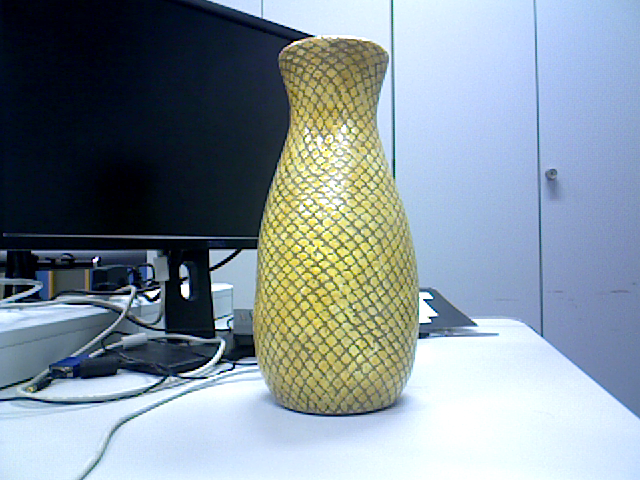
\includegraphics[width=0.45\textwidth]{figures/methodology/inpainting_rgb.png}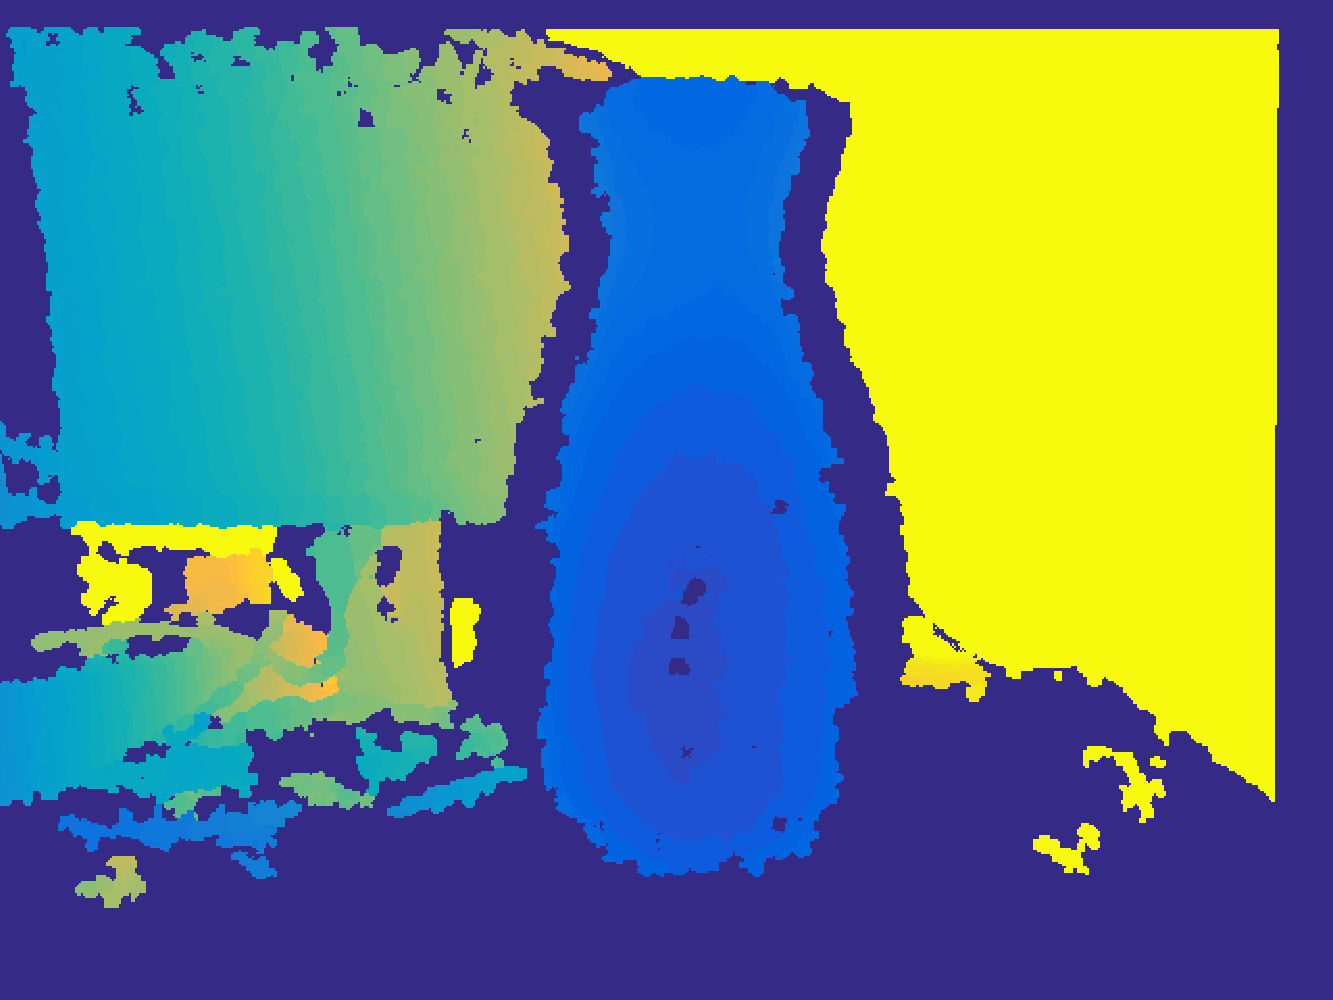
\includegraphics[width=0.45\textwidth]{figures/methodology/inpainting_depth.pdf}
% \caption{dd}
% \label{fig:inpainting1}
%\end{figure}

Image inpainting itself is a very mutual area and has been widely applied as a useful tool for many modern computer vision applications, e.g, restore the damaged parts of ancient paintings, or remove unwanted texts or objects in a photography~\cite{bertalmio2000image}. 
Since the idea of image inpainting is to automatically replace the lost or undesired parts of an image with the neighbouring information by interpolating, we were inspired to apply it to fill in the missing depth information (Fig.~\ref{fig:inpainting1}).

\begin{figure}[!htbp]
\centering
\subfigure[RGB image]{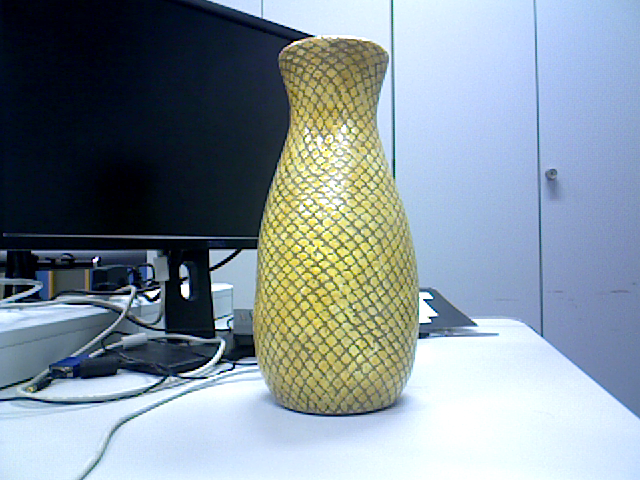
\includegraphics[width=0.45\linewidth]{figures/methodology/inpainting_rgb.png}}
\subfigure[Input depth image]{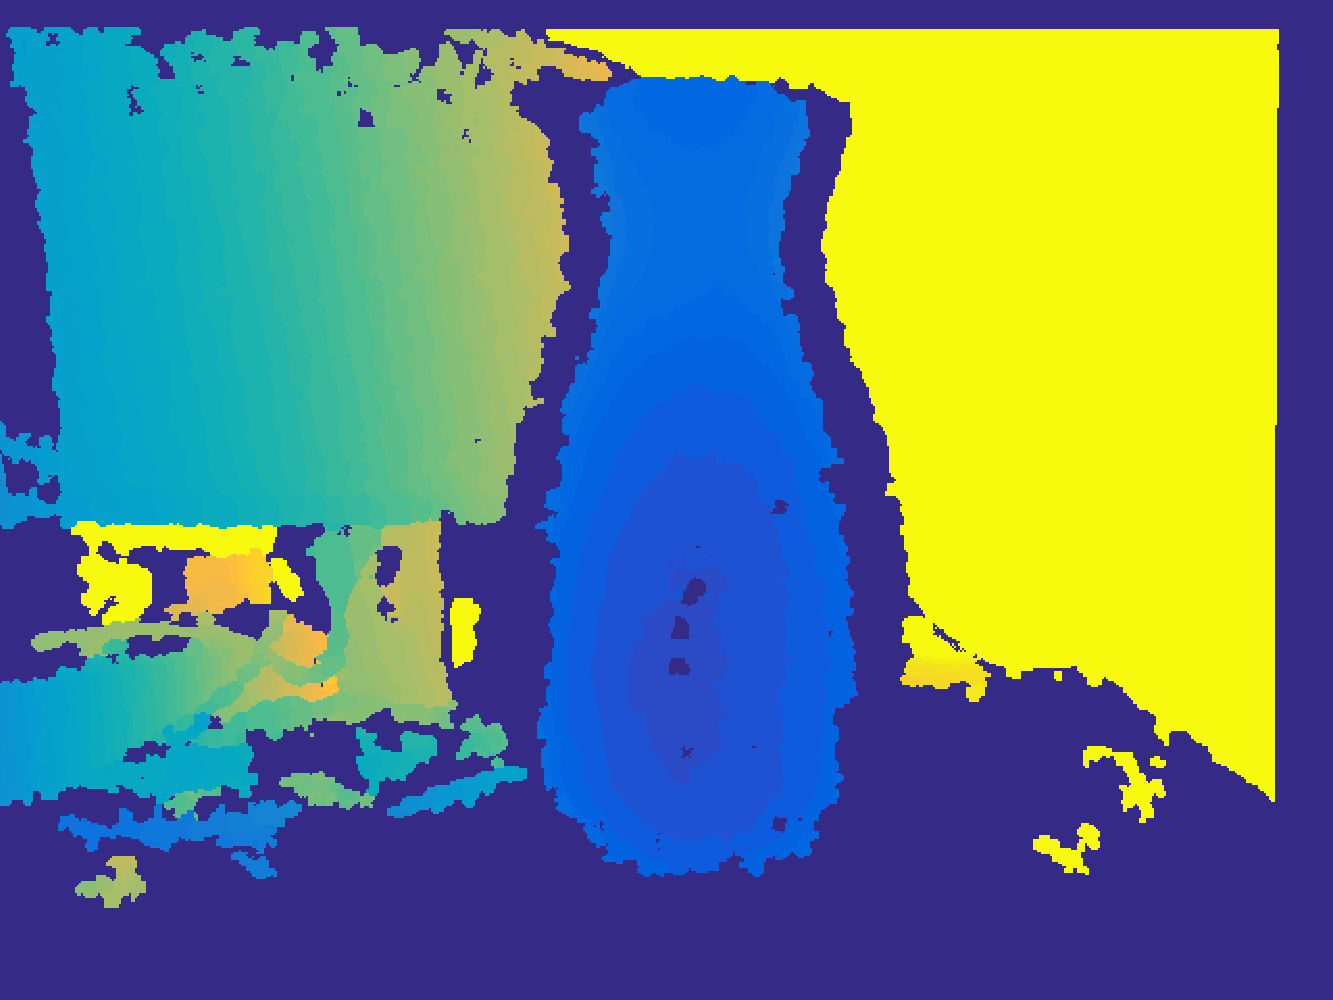
\includegraphics[width=0.45\linewidth]{figures/methodology/inpainting_depth.pdf}}
\caption{The input RGB and depth image of a vase. The depth map in (b) is visualized using color from blue (near) to yellow (far).}
\label{fig:inpainting1}
\end{figure}

It should be noted that, the depth inpainting is applied to the input noisy image so there is no need to use some powerful and advanced algorithms.
The only request is to fill the missing areas with inexpensive computational time.

The general mathematical form of a classic inpainting algorithm~\cite{bertalmio2000image} can be written as follows

\begin{equation}\label{eq:method_inpaint1}
I^{t+1}(i,j) = I^{t}(i,j) + \mu U^{t}(i,j), \forall(i,j)\in \Omega
\end{equation}
where $I(i,j)$ is the pixel value in image $I$, $t$ is the artificial time step, $\mu$ is the updating rate, $U$ is the update information and $\Omega$ are the area with missing information.

To build the update map $U$ in each time step, there are two principles that~\cite{bertalmio2000image} follow.
One is the inpainted values inside $\Omega$ should be as smooth as possible. 
The other is the lines reaching the edge of $\Omega$ should be continued and cross the missing area, while the values in $\Omega$ should be propagated from the nearest neighbours of $\Omega$ along the lines.

Again, due to the fact that our input depth images have poor quality, the lines arriving at the boundary $\delta \Omega$ may be incorrect or produced by the noises.
Thus, it is reasonable that our initial depth inpainting problem focuses on the smooth propagation from the neighbours and fill in the holes.

In each pixel $(x_0, y_0)$ inside $\Omega$, $U$ can be modelled as a discrete four-neighbour Laplacian operator:
\begin{equation}
\begin{split}
U(x_0, y_0) = \Delta I
		        = 4I(x_0, y_0) - I(x_0 + 1, y_0) - I(x_0 - 1, y_0) - I(x_0, y_0+1) - I(x_0 , y_0 -1)
\end{split}
\end{equation}
Now the inpainting problem in Eq.~\ref{eq:method_inpaint1} can be represented as a minimization problem: 
\begin{equation}
\min \iint\limits_{\Omega} |U(x,y)|^2 dxdy 
\end{equation}
This problem can be reformulated to a typical linear equation in matrix form:
\begin{equation}
\mathbf{Ax=b}
\end{equation}
Assuming $n$ is the number of pixel inside $\Omega$ and $m$ is the sum of $n$ and the number of neighbouring pixel around the boundary $\delta \Omega$, $\mathbf{A}$ is a $m\times n$ Laplacian matrix, $\mathbf{b}$ is a $m\times1$ vector containing all the known boundary depth values and the $0$ inside $\Omega$.
Solving the linear equation with simple least square method, we can acquire the inpainted values.
With our this naive image inpainting algorithm, we can fill the holes on the depth image as shown in Fig.~\ref{fig:pre-processing}.

%----------------------------------------------
\subsection{Depth denoising}
%----------------------------------------------
the depth images acquired from the RGB-D cameras with moderate price usually contain various noises. 
As a standard pre-processing method, the image denoising technique is also applied to our input inpainted depth map.
Similar to the state-of-the-art depth refinement methods~\cite{zhang2012edge, or2015rgbd, han2013high, or2016real, haque2014high, yu2013shading}, bilateral fitering~\cite{tomasi1998bilateral} is used as our depth pre-processing smoother. 

The advantages of bilateral filter is reducing the noise while preserving the edge in the input image. 
More than a regular Gaussian smooth filter, which uses only the difference of the image values (depth in our case) between the center pixel the neighbours, the bilateral filter also utilizes the space difference as a reference to build up the weighting function.
The filtered pixel value can be modelled as a weighted sum of neighbouring pixels:
\begin{equation}
\hat{I}(\mathbf{x}) = \frac{1}{W}\sum_{\mathbf{y} \in \mathcal{N}} I(\mathbf{y})e^{-(\frac{\lVert I(\mathbf{x}) - I(\mathbf{y})\rVert^2}{2\sigma_r^2} + \frac{\lVert \mathbf{x} - \mathbf{y}\rVert^2}{2\sigma_d^2})}
\end{equation}
where $\hat{I}(\mathbf{x})$ is the filtered value at pixel $\mathbf{x}$, $\mathcal{N}$ represents the neighbouring pixels with $\mathbf{x}$ in the center, and $W$ is the the sum of the all the weights. 
The smoothed result on our input depth image is shown in Fig.~\ref{fig:pre-processing}.

\begin{figure}[!htbp]
\centering
\subfigure[Input depth]{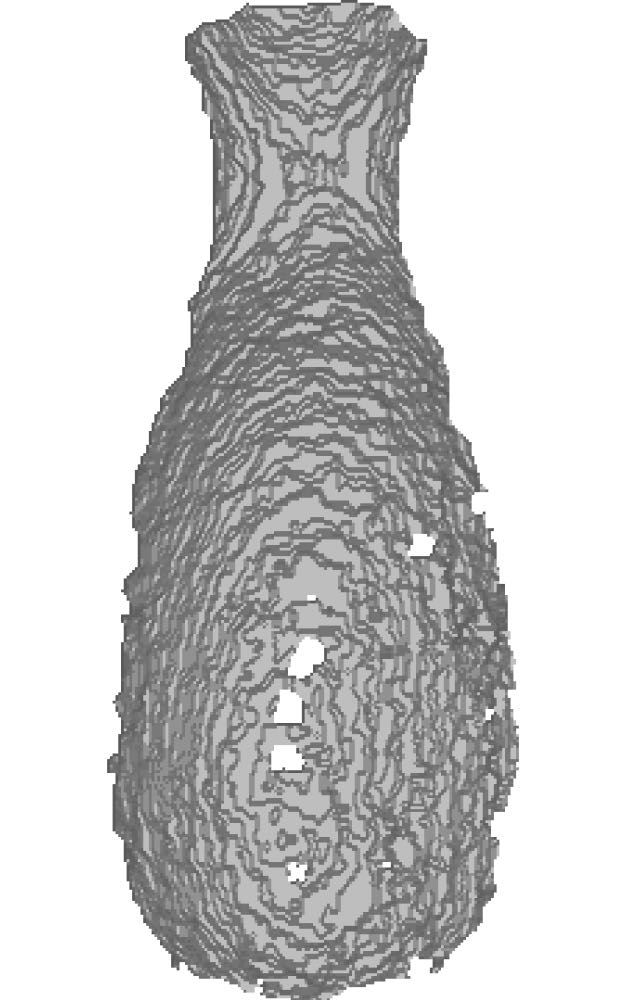
\includegraphics[width=0.30\linewidth]{figures/methodology/inpainting_shape_before.pdf}}
\subfigure[After inpainting]{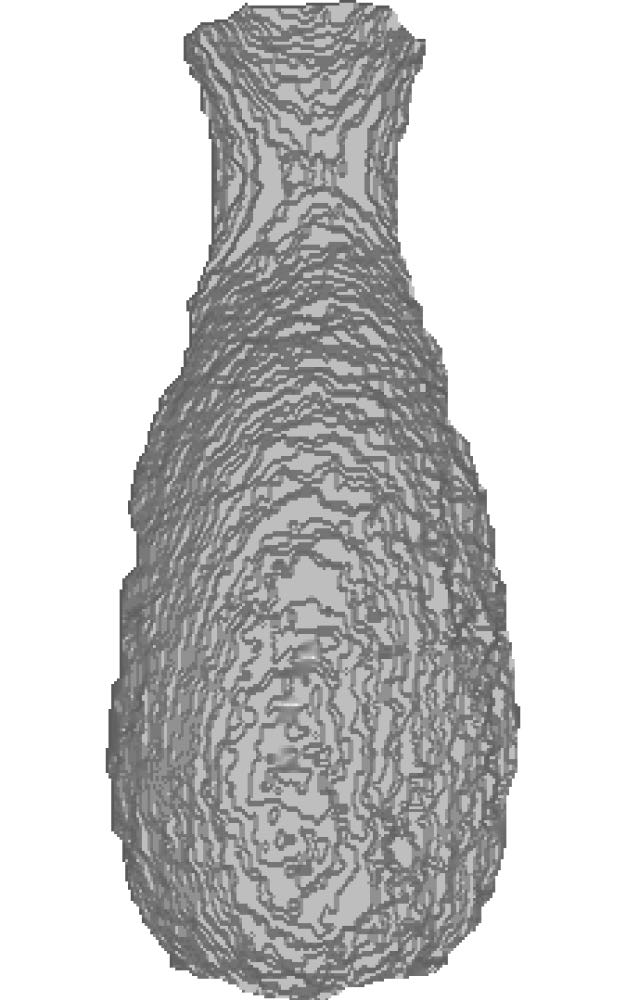
\includegraphics[width=0.30\linewidth]{figures/methodology/inpainting_shape_after.pdf}}
\subfigure[After smoothing]{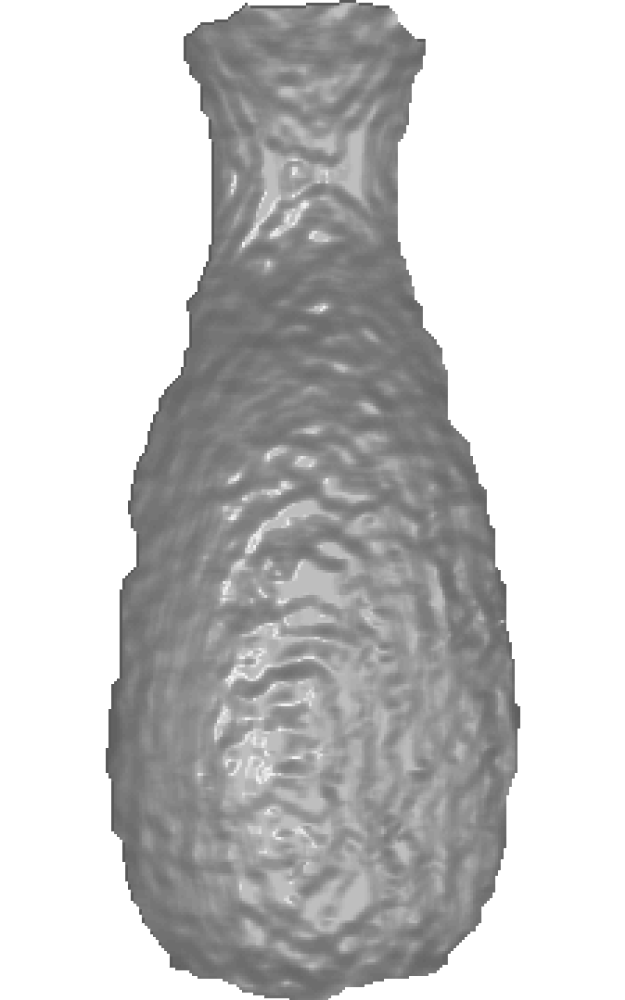
\includegraphics[width=0.30\linewidth]{figures/methodology/smooth_shape_after.pdf}}
\caption{Illustrations for the pre-processing on the depth of the vase.}
\label{fig:pre-processing}
\end{figure}

After the pre-processing procedure, we have an initial smooth and inpainted depth image. 
It will be used as the input of all the depth refinement methods detailed in the following sections.

%%%%%%%%%%%%%%%%%%%%%%%%%%%%%%%%%%%%%%%%%%%%
\section{RGBD-Fusion Like method}
%%%%%%%%%%%%%%%%%%%%%%%%%%%%%%%%%%%%%%%%%%%%
RGBD-Fusion is a state-of-the-art depth recovery method proposed by Or-El \emph{et al.}~\cite{or2015rgbd} in 2015.
This novel method is adequate for natural scene illumination and able to enhance the depth map much faster than other methods.
It is reasonable to gain a comprehensive understanding in the field of depth refinement by implementing this method with our own idea inside.

It is worth mentioning that we didn't just follow the paper step by step without injecting any our own ideas.
For example, instead of estimating the pixel-wise ambient light with a separate energy function, we jointly calculated all four first-order spherical harmonics parameters (3 for point-source light direction and 1 for ambient light) with a simple fast least square, and the results have only negligible difference.
And throughout the whole estimation process of light, albedo and depth, we only used the information within the given mask which also speeded up the algorithm.
This is the reason we call our first method "RGB-Fusion Like" method.

The natural uncalibrated illumination condition means the light is no longer a point light source, thus a Lambertian model is not sufficient. 
Basri and Jocobs~\cite{basri2003lambertian} has found that low order spherical harmonics (SH) model can well set out the irradiance of the diffused objects under the natural scene.
More specifically, the first-order SH model can capture 87.5\% of natural lighting, whose form is extended from the Lambertian model:
%$$$$$$$$$$$$$$$$$$
\begin{equation}\label{eq:rgbd_light_model}
I(x,y) = \rho(x,y)(\mathbf{l}^\top \mathbf{n}(x,y) + \varphi)
\end{equation}
%$$$$$$$$$$$$$$$$$$
where $I : \mathcal{M}\rightarrow \mathbb{R}^C$ is the irradiance of the objects, which is represented as the intensity values. 
$\rho : \mathcal{M}\rightarrow \mathbb{R}^C$ is the albedo, $\mathbf{l}^\top = \begin{pmatrix} l_x & l_y & l_z \end{pmatrix}$ describes the light direction and $\varphi$ represents the ambient light.
$\mathbf{n} : \mathcal{M}\rightarrow \mathbb{R}^3$ is the surface normal, which is dependent on the depth $z$.
We define that $C = 1$ represents the grayscale image while C = 3 for color image. 
$(x,y) \in \mathcal{M}$ represents the pixel coordinate inside the given mask $\mathcal{M}$ of an object.
Eq.~\ref{eq:rgbd_light_model} can be rewritten as:
%$$$$$$$$$$$$$$$$$$
\begin{equation}\label{eq:rgbd_light_model2}
I(x,y) = \rho(x,y) \; \mathbf{s}^\top \tilde{\mathbf{n}}(x,y)
\end{equation}
%$$$$$$$$$$$$$$$$$$
where
%$$$$$$$$$$$$$$$$$$
\begin{equation}
\mathbf{s} = \begin{pmatrix}\mathbf{l} \\ \varphi \end{pmatrix} 
 \; \; 
\tilde{\mathbf{n}}(x,y) = \begin{pmatrix}\mathbf{n}(x,y) \\ 1\end{pmatrix}
\end{equation}
%$$$$$$$$$$$$$$$$$$
$\mathbf{s}$ is the first-order SH parameters. It should be mentioned that the 1st-order SH model is used as the fundamental model throughout the whole methodology part.

After introducing the preliminary knowledge, the overall energy function for the RGBD-Fusion like method which can jointly estimate lights, albedo and depth is described below:
%$$$$$$$$$$$$$$$$$$
\begin{equation}\label{eq:rgbd_energy_rough}
    \begin{split}
        E(\rho, z, \mathbf{s}) = \; \mathop{\sum \sum}_{(x,y) \in \mathcal{M}} | I(x,y) - &\rho(x,y) \mathbf{s}^\top\tilde{\mathbf{n}}(x,y) |^2 
        + \lambda_{\rho} \mathop{\sum \sum}_{(x,y) \in \mathcal{M}} \sum_{k \in \mathcal{N}} |\omega_k(x,y) (\rho(x,y) - \rho_k) |^2 \\
        &+ \lambda_z \mathop{\sum \sum}_{(x,y) \in \mathcal{M}} | z(x,y) - z_0(x,y)|^2 + 
        \lambda_l \mathop{\sum \sum}_{(x,y) \in \mathcal{M}} |\Delta z(x,y) |^2
    \end{split} 
\end{equation}
%$$$$$$$$$$$$$$$$$$
For the sake of simplicity, we will use $\lVert \boldsymbol{\cdot} \rVert_2^2 =\mathop{\sum \sum}\limits_{(x,y) \in \mathcal{M}}(\cdot)^2$ to reshape the equation, and then $I$ and $\rho$ are vectorized to $\mathbb{R}^m$ within the mask, while $\tilde{\mathbf{n}} \in \mathbb{R}^{m\times 4} $. $m$ is the number of pixel inside the mask $\mathcal{M}$.
So Eq.~\ref{eq:rgbd_energy_rough} can be reformulated as:
%$$$$$$$$$$$$$$$$$$
\begin{equation}\label{eq:rgbd_energy}
	E(\rho, z, \mathbf{s}) = \; \lVert I - \rho \cdot \; \tilde{\mathbf{n}}(z)\mathbf{s} \rVert^2_2 + \lambda_{\rho} \lVert \sum_{k \in \mathcal{N}} \omega_k (\rho - \rho_k) \rVert^2_2 + \lambda_z \lVert z - z_0\rVert^2_2 + \lambda_l \lVert \Delta z \rVert^2_2
\end{equation}
%$$$$$$$$$$$$$$$$$$

The function consists of a SFS term, an albedo anisotropic Laplacian term, a depth data fidelity term and a depth isotropic Laplacian term. 
Now we will go into the details step by step.

%----------------------------------------------
\subsection{Light estimation}
%----------------------------------------------
Here the surface normal $\mathbf{n}$ is formulated with orthographic projection, i.e. 
\begin{equation}\label{eq:rgbd_normal}
	\mathbf{n}(x,y) = \frac{1}{\sqrt{1 + |\nabla z(x,y)|^2}}
	\begin{pmatrix} 
		 \nabla z(x,y)\\ 
		 -1
	 \end{pmatrix}
\end{equation}
$\nabla z(x,y)$ represents the gradient of depth image $z(x,y)$ in $x$ and $y$ directions.
Since we have the input depth from pre-processing, initial $\mathbf{n}_0$ is known.

In the sense of intrinsic image decomposition, an image can be decomposed as the product of albedo and shading, so we can treat $\mathbf{s}^\top \tilde{\mathbf{n}}(x,y) $ in Eq.~\ref{eq:rgbd_light_model2} as the shading.

To compute the spherical harmonics parameters, we assume the albedo $\rho$ equals to $1$ for each pixel. 
Since there are known intensity value and surface normal in each pixel within the mask, we will have an overdetermined least square problem from the energy in Eq.~\ref{eq:rgbd_energy}: 
\begin{equation}\label{eq:rgbd_light_estimate}
\min_{\mathbf{s}} \; \lVert \tilde{\mathbf{n}} \mathbf{s} - I \rVert^2_2
\end{equation}
This process only need to be applied once at the beginning of the process since the least squares is not sensitive to the details on the surface, thus the estimation from the smooth surface is enough.

%----------------------------------------------
\subsection{Albedo estimation}\label{sec:rgbd_albedo_estimation}
%----------------------------------------------
As mentioned in Chapter~\ref{chap:background}, many depth recovery methods based on SFS or photometric stereo techniques assume constant or uniform albedo.
Such assumption does not fit in with the real-world objects, and hence, they perform poorly on the shape estimation for multi-albedo cases.
In order to acquire a satisfying shape outcome, an effective multi-albedo estimation process is a matter of importance.

We know from Eq.~\ref{eq:rgbd_light_model} that, assuming we have the knowledge of input intensity and estimated shading, the albedo image can be directly obtained from $I/S$.
However, such albedo is prone to the overfitting, which make the acquired albedo contain all the undesired spatial layout details.
This is due to the fact that both input image $I$ and the surface normal $\mathbf{n}$ are noisy.
To resolve the overfitting problem, we should impose some restrictions on the estimation of albedo.
A large amount of our daily objects have piecewise smooth appearance, which means most pieces of a layout are dominated by certain colors.
Therefore, a prior that emphasizes the piecewise smoothness on the albedo should be defined.

The albedo of an object can be roughly divided to several pieces with different intensities, which can be treated as the image segmentation problem to some extend. 
Thus, we should refer to some classic variational segmentation methods and adapt the edge preserving smoothness term to our problem.
Similar to the idea in~\cite{casaca2014laplacian}, an anisotropic Laplacian term is imposed to estimate the albedo.
Now, the SH parameters $\mathbf{s}$ and the surface normal $\mathbf{n}$ are fixed, the overall regularized minimization problem in Eq.~\ref{eq:rgbd_energy} is:

\begin{equation}\label{eq:rgbd_albedo_estimate}
	\min_{\rho} \; \lVert \rho \cdot \tilde{\mathbf{n}} \mathbf{s} - I\rVert^2_2 + \lambda_{\rho} \lVert \sum_{k \in \mathcal{N}} \omega_k (\rho - \rho_k) \rVert^2_2
\end{equation}
where $k$ indicates the neighbouring index of a certain pixel, which 4-connected set is chosen for $\mathcal{N}$ in our case. 
The weight $\omega_k$ is defined as below, and it is dependent to two parameters $\sigma_I$ and $\sigma_z$ which accounts for the discontinuity in both intensity and depth.
\begin{equation}
	\omega_k=\exp\Bigg(-\dfrac{\lVert I - I_k \rVert^2_2}{2\sigma_I^2} -\dfrac{\lVert z - z_k \rVert^2_2}{2\sigma_z^2}\Bigg)
\end{equation}

%----------------------------------------------
\subsection{Depth enhancement}
%----------------------------------------------
After acquiring the first-order spherical lighting parameters $\mathbf{s}$ and the albedo $\rho$, we can refine our depth with the help of Eq.~\ref{eq:rgbd_light_model} and Eq.~\ref{eq:rgbd_normal}.
Now our minimization problem with respect to the depth $z$ in Eq.~\ref{eq:rgbd_energy} can be written as below. 
The data fidelity term is applied to resolve the SFS ambiguities and enables our refined surface close to the input. The Laplacian smoothness term makes sure that there is no strong discontinuity in the output. 
\begin{equation}\label{eq:rgbd_depth_refine}
	\min_{z} \; \lVert \rho \cdot \tilde{\mathbf{n}}(z) \mathbf{s} - I \rVert^2_2 + \lambda_z \lVert z - z_0\rVert^2_2 + \lambda_l \lVert \Delta z \rVert^2_2
\end{equation}
where $z_0$ is the input depth and $\Delta$ represents the  Laplacian operator. 
It can be easily noticed that this introduced function is non-linear because the normal in our SFS term contains a denominator related to the depth gradient. 
Many optimization methods can be applied to solve the non-linear problem, e.g. Levenberg-Marquardt algorithm or ADMM, but they are not suitable in our application due to expensive computational time. 
Here a "fixed point" method which is similar to iteratively reweighted least square (IRLS) has been introduced to deal with our problem efficiently. 

The idea of the fixed-point approach is in each iteration, the normalizer in the surface normal can be treated as a weighting term and determined by the depth from last iteration.
With the help of this trick, the normalizer is known and Eq.~\ref{eq:rgbd_depth_refine} is linear again.
We can solve the linear system using any fast linear optimization method.
In each iteration $t$, this process can be represented element-wise as follows:
\begin{equation}
	\begin{split}
		\mathbf{n}^{(t)}(z^{(t)}, z^{(t-1)}) &= w(z^{(t-1)})
		\begin{pmatrix} 
			 \nabla z^{(t)}\\ 
			 -1
	         \end{pmatrix}\\
	         w(z^{(t-1)}) &=  \frac{1}{\sqrt{1 + |\nabla z^{(t-1)}|^2}}
	\end{split}
\end{equation}
And now the depth refinement problem in Eq.~\ref{eq:rgbd_depth_refine} is reformulated as below in each iteration:

\begin{equation}\label{eq:rgbd_depth_refine2}
	\min_{z^{(t)}} \; \lVert \rho \cdot \tilde{\mathbf{n}}(z^{(t)}, z^{(t-1)}) \mathbf{s} -I\rVert^2_2 + \lambda_z \lVert z^{(t)} - z_0\rVert^2_2 + \lambda_l \lVert \Delta z^{(t)} \rVert^2_2
\end{equation}
As long as the energy decreases in each iteration, the process is repeated.

To sum up the approach in this section, it should be noted that the SFS term in the overall energy (Eq.~\ref{eq:rgbd_energy} was used as a core in all light, albedo and depth estimation.
The whole process of RGBD-Like method has been described in Alg.~\ref{alg:rgbd_fusion} and some real-world results are shown in Fig.~\ref{fig:rgbd_illustration}.



\begin{algorithm}[!htbp]
	\begin{algorithmic}[1]
  		\caption{\textbf{RGBD-Fusion Like Depth Refinement}}
		\label{alg:rgbd_fusion}
		 \renewcommand{\algorithmicrequire}{\textbf{Input:}}
		 \renewcommand{\algorithmicensure}{\textbf{Output:}}
		 \REQUIRE Initial depth image $z_0$, RGB image $I$
		 \vspace{1.8mm}
		 \STATE Estimate SH parameter, $\mathbf{s} = \argmin \limits_{\mathbf{s}} \; E(\rho = 1, z_0)$ \COMMENT{Eq.~\ref{eq:rgbd_light_estimate}}
		 \STATE Estimate albedo, $\rho = \argmin \limits_{\rho} \; E(z_0, \mathbf{s})$ \COMMENT{Eq.~\ref{eq:rgbd_albedo_estimate}}
		 \STATE t = 1, $z^{(t-1)} = z_0$
		 \vspace{1.8mm}
		  \WHILE {$ E(\rho, z^{(t)}, \mathbf{s}) - E(\rho, z^{(t-1)}, \mathbf{s}) < 0$}
		   \vspace{1.8mm}
			  \STATE $z^{(t)} = \argmin \limits_{z} E(\rho, z, \mathbf{s})$ \COMMENT{Eq.~\ref{eq:rgbd_depth_refine2}}
		          \STATE $t := t + 1$
		 \vspace{1.8mm}
		  \ENDWHILE
		  \ENSURE  Refined depth image $z^{(t)}$
	\end{algorithmic}
\end{algorithm}

%&&&&&&&&&&&&&&&&&&&&&&&&&
\begin{figure}[!ht]
\centering
\setlength{\tabcolsep}{0.1em} % column spacing
 {\renewcommand{\arraystretch}{0.6}% row spacing
\begin{tabular}{c|c c c}
   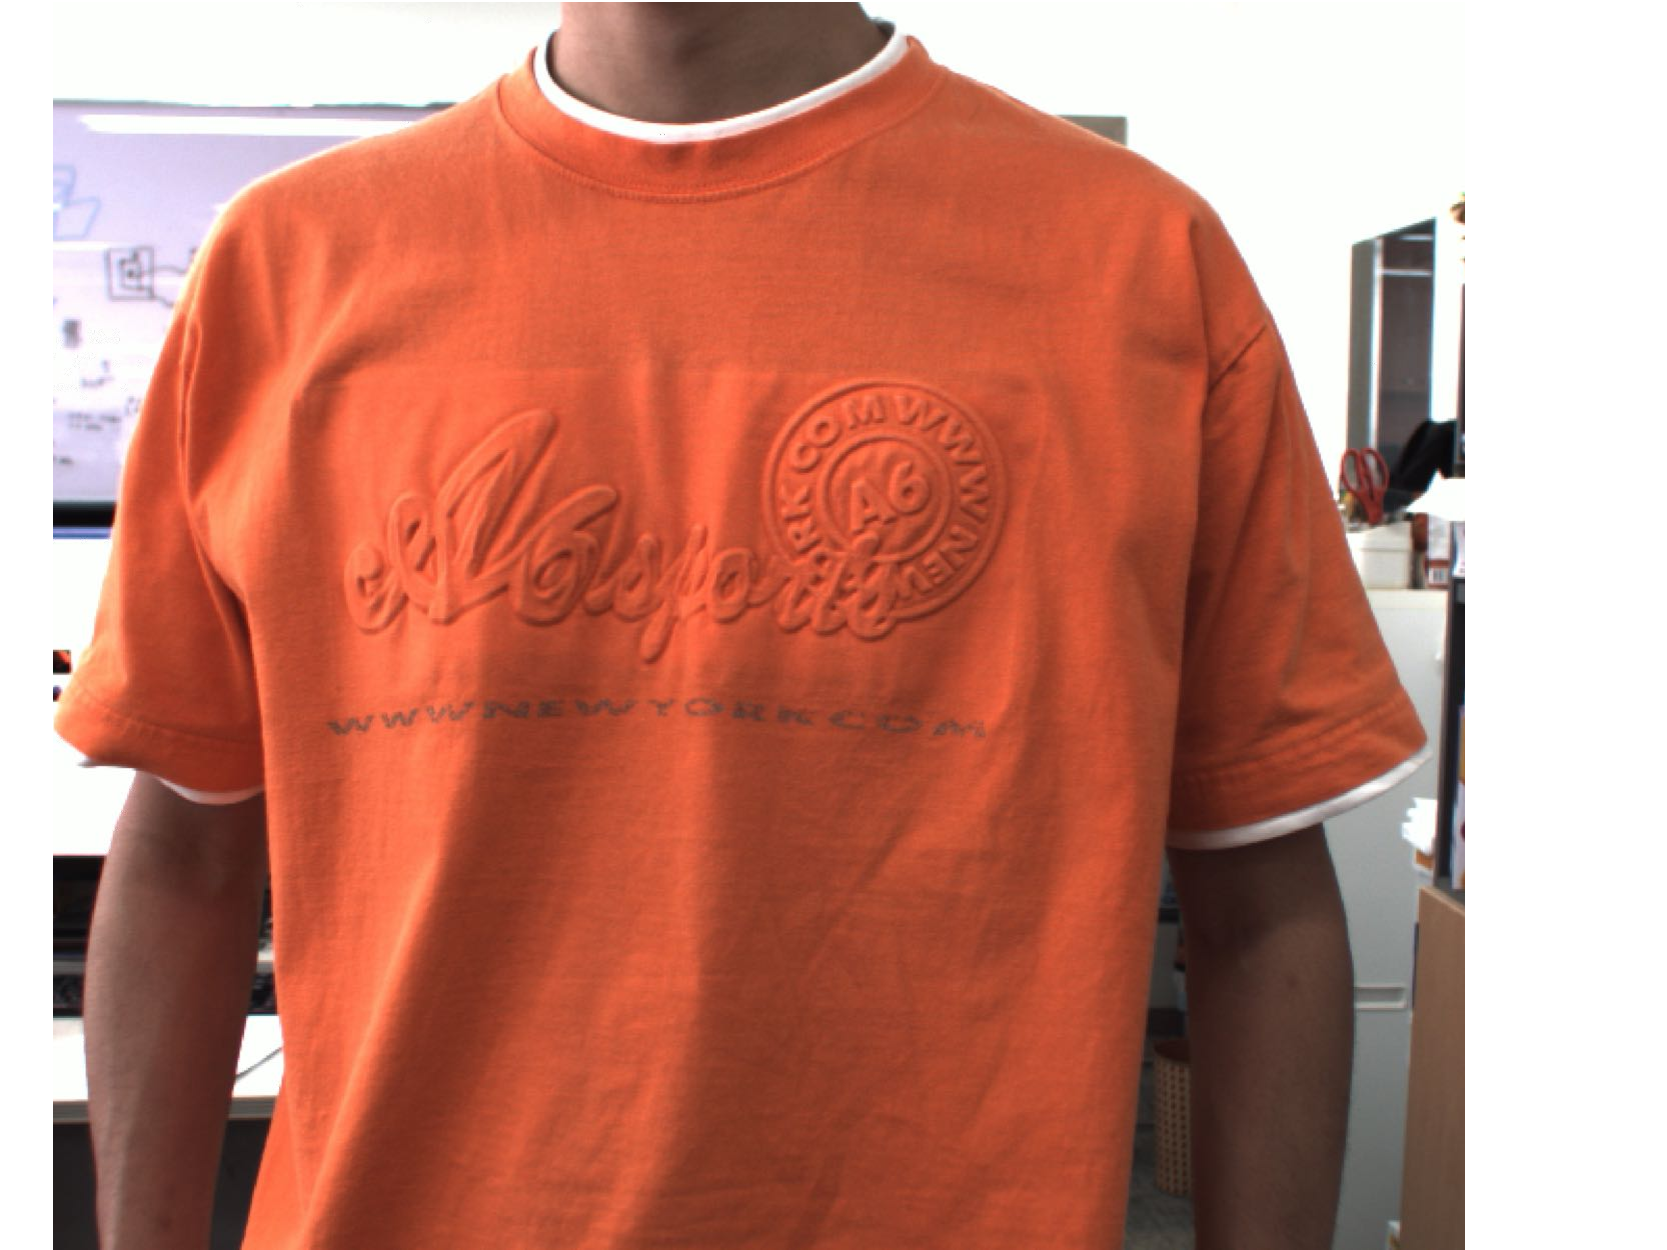
\includegraphics[height = 0.19\linewidth]{figures/methodology/rgbd_body_rgb.pdf} \hspace{0.05cm}
   &
   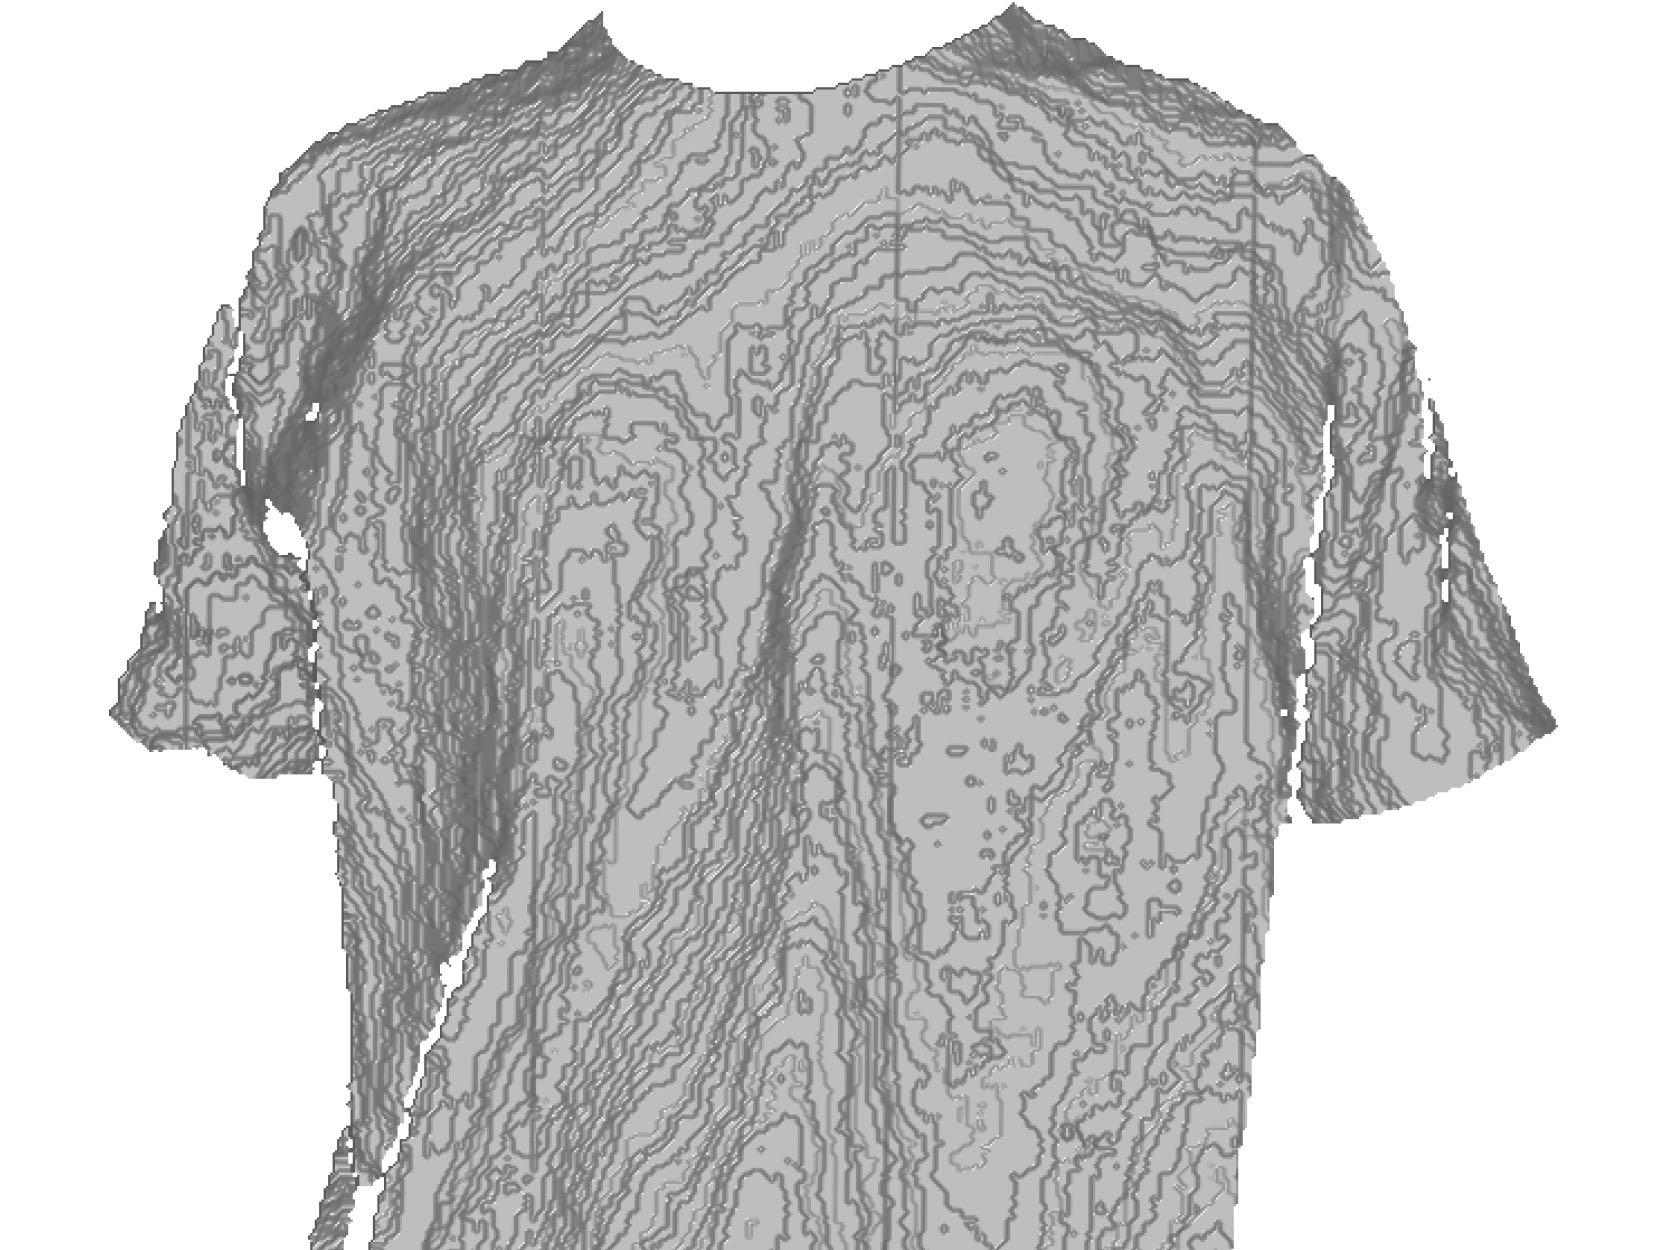
\includegraphics[height = 0.19\linewidth]{figures/methodology/rgbd_body_shape_init.pdf} &
   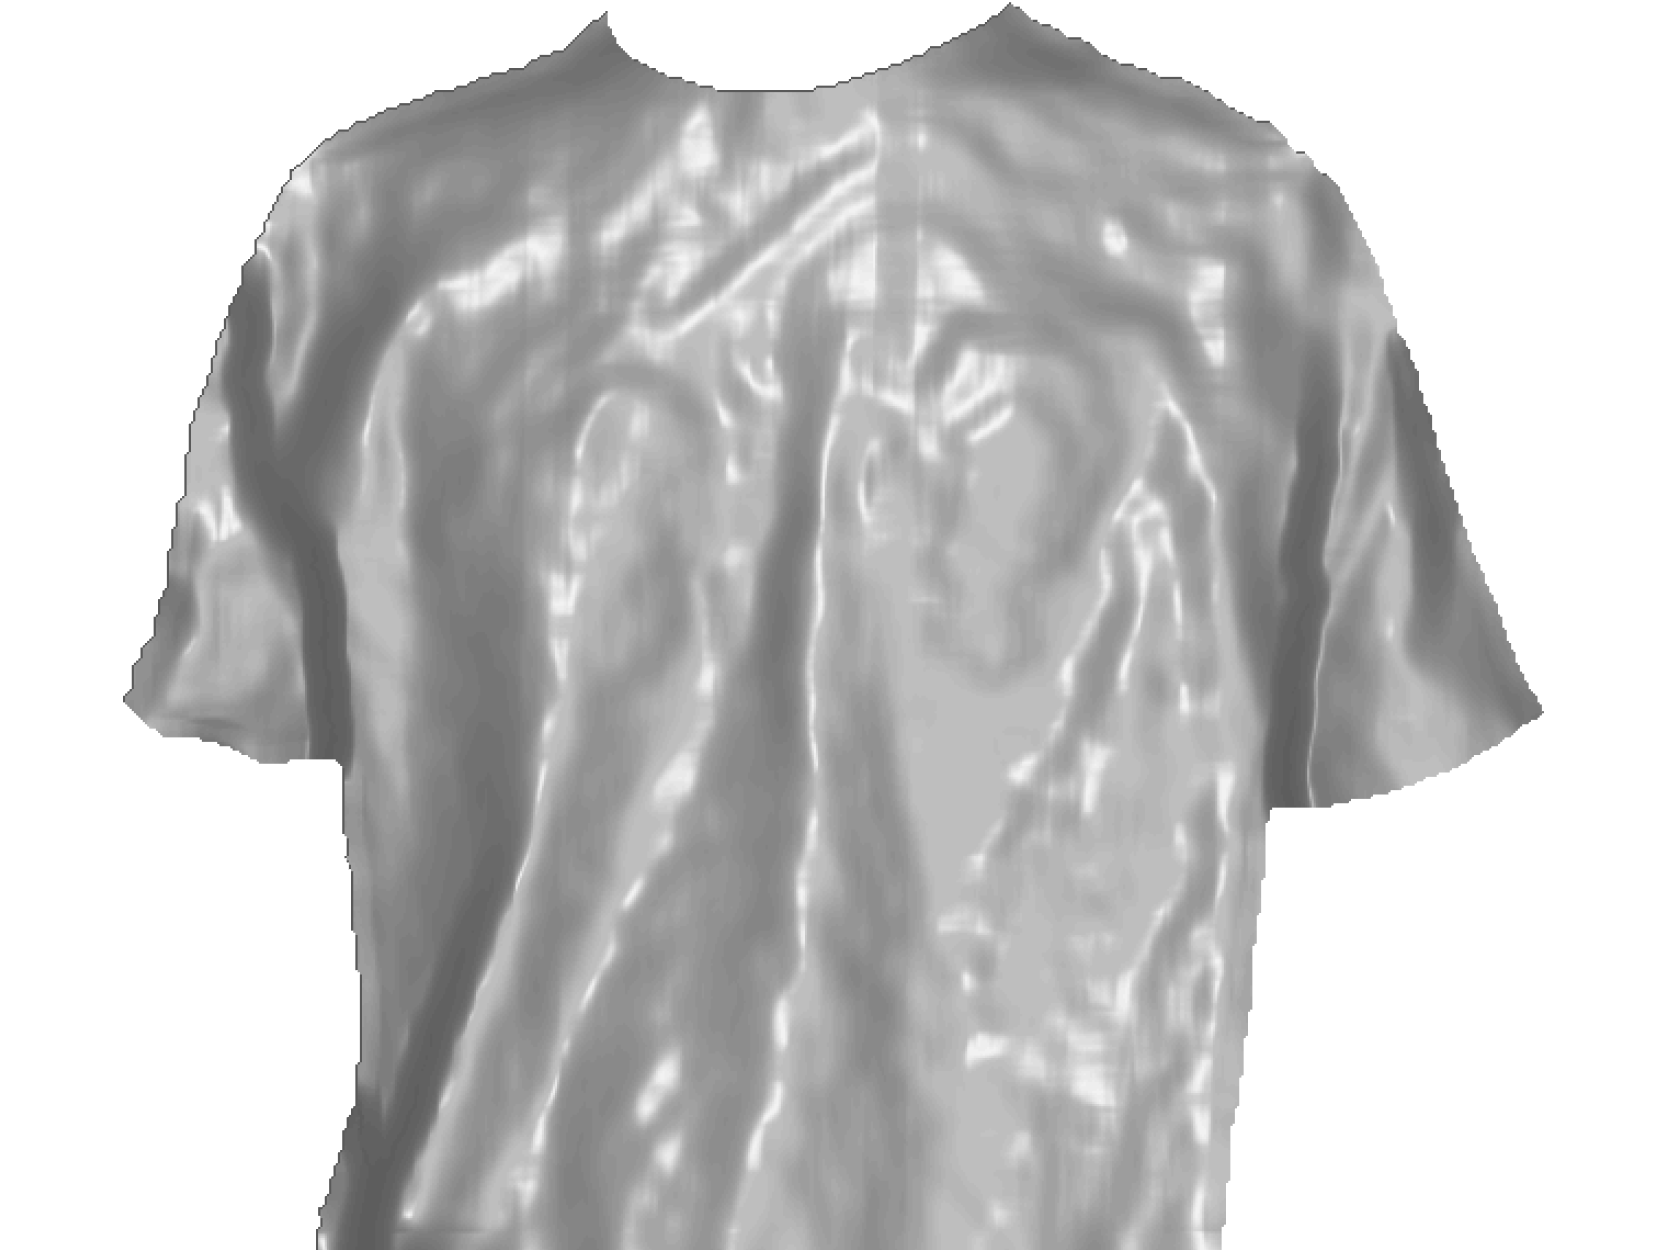
\includegraphics[height = 0.19\linewidth]{figures/methodology/rgbd_body_shape_smooth.pdf} &
   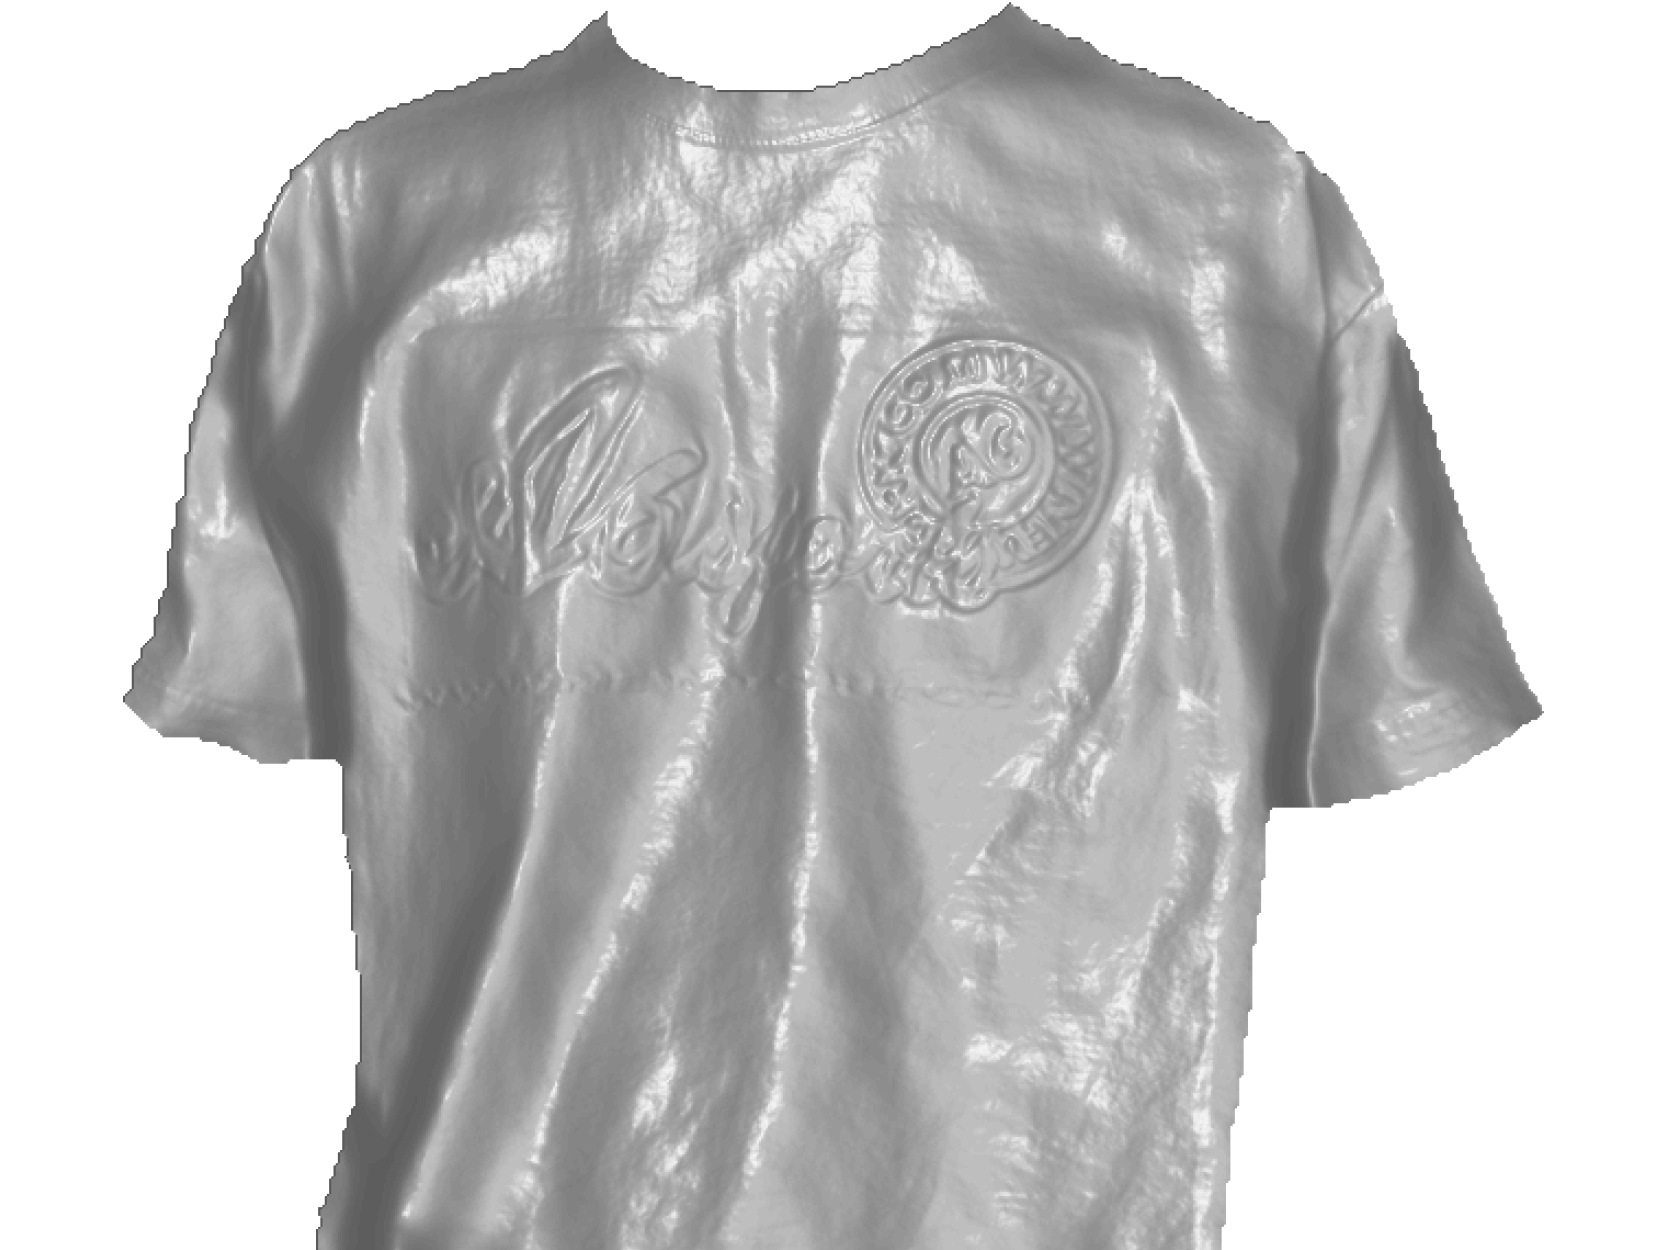
\includegraphics[height = 0.19\linewidth]{figures/methodology/rgbd_body_shape.pdf} \\
   
   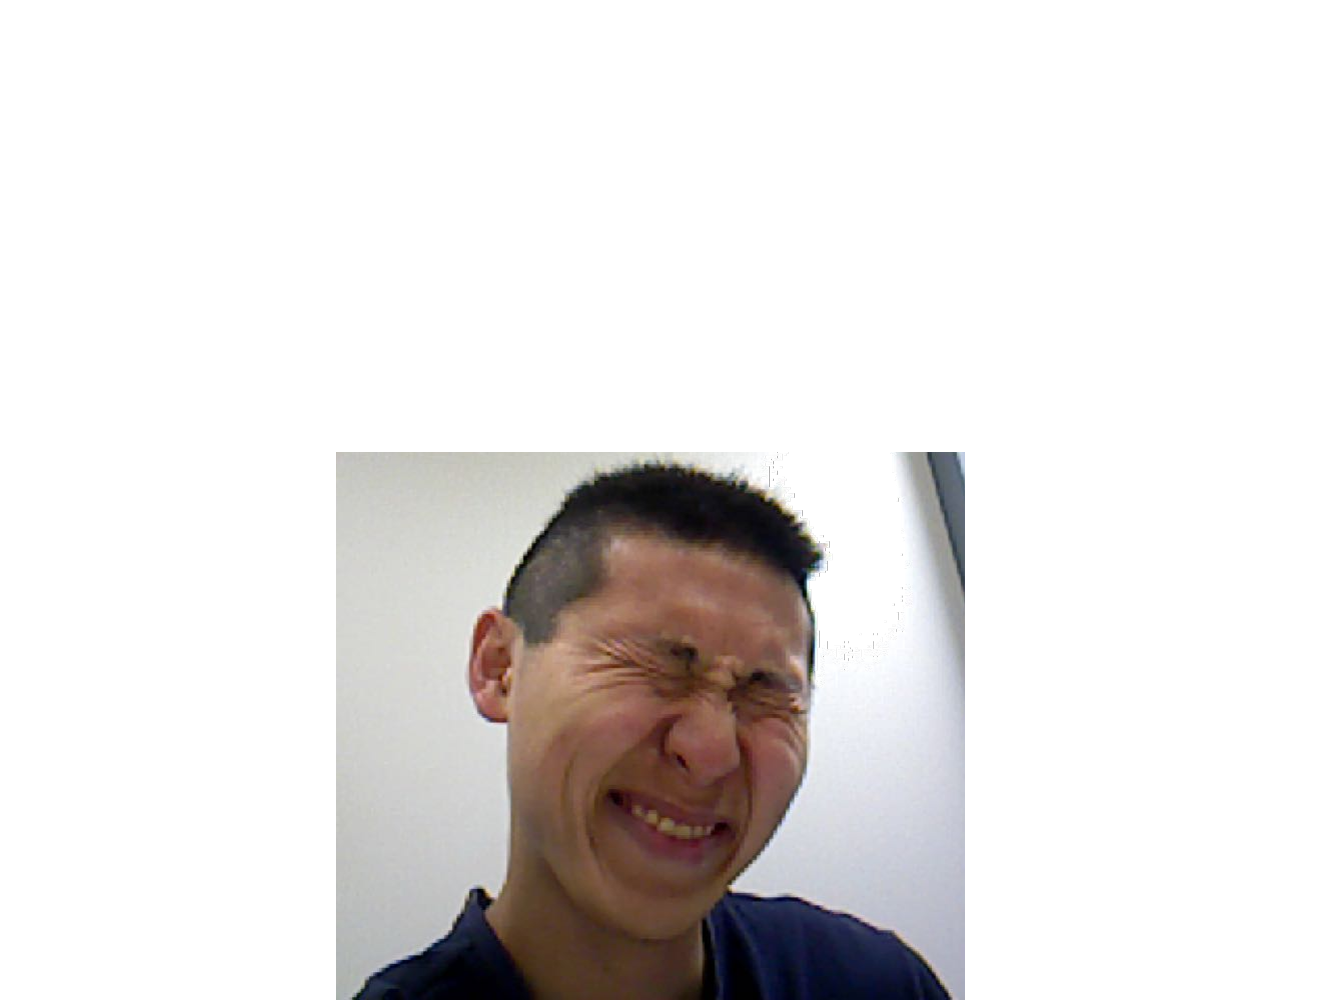
\includegraphics[height = 0.19\linewidth]{figures/methodology/rgbd_face_rgb.pdf} \hspace{0.05cm}
   &
   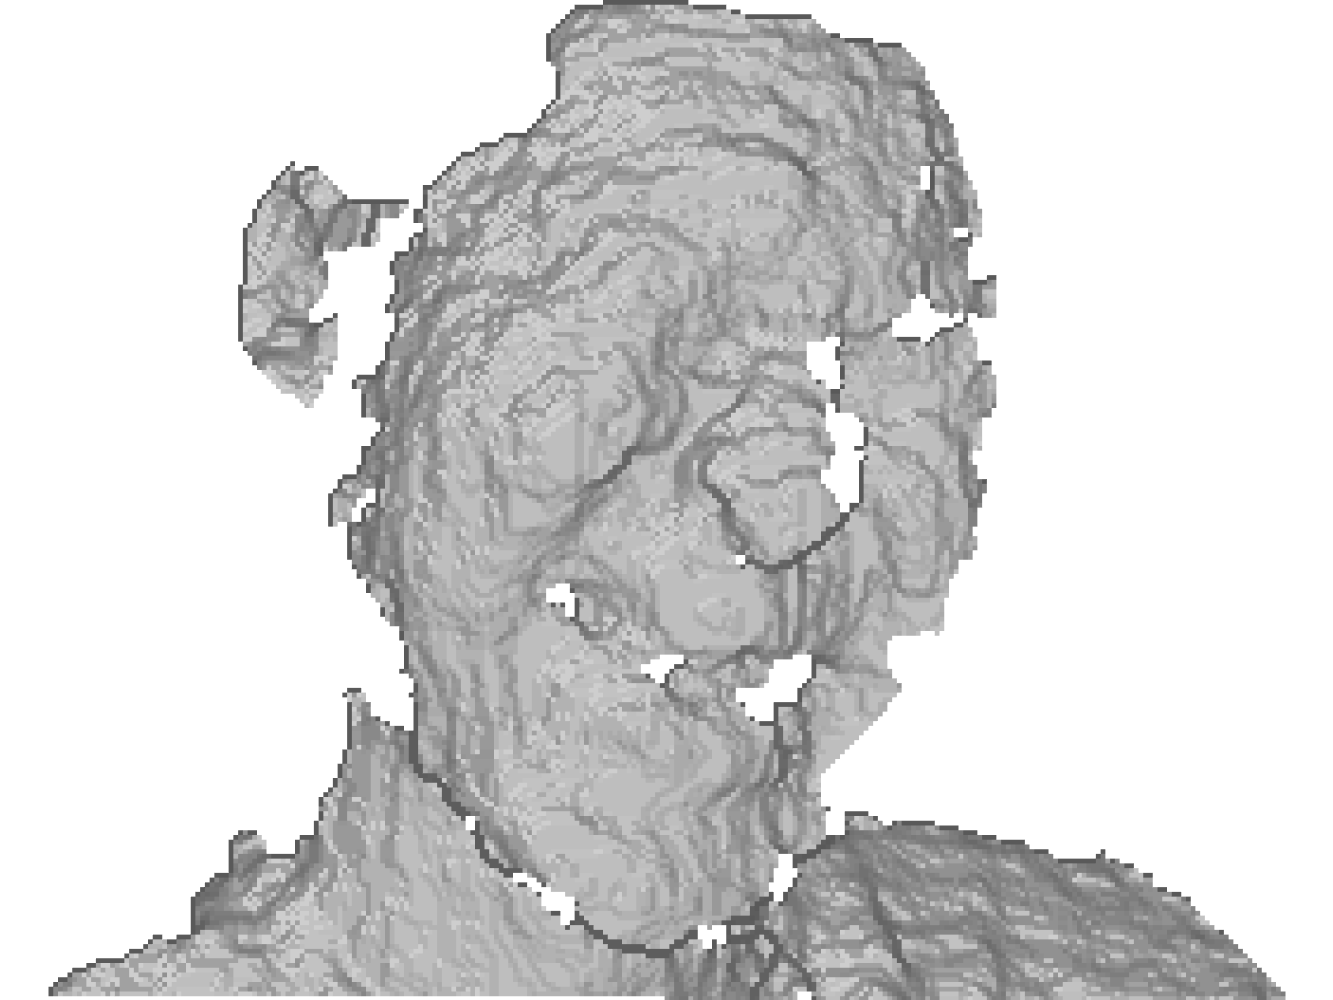
\includegraphics[height = 0.19\linewidth]{figures/methodology/rgbd_face_shape_init.pdf} &
   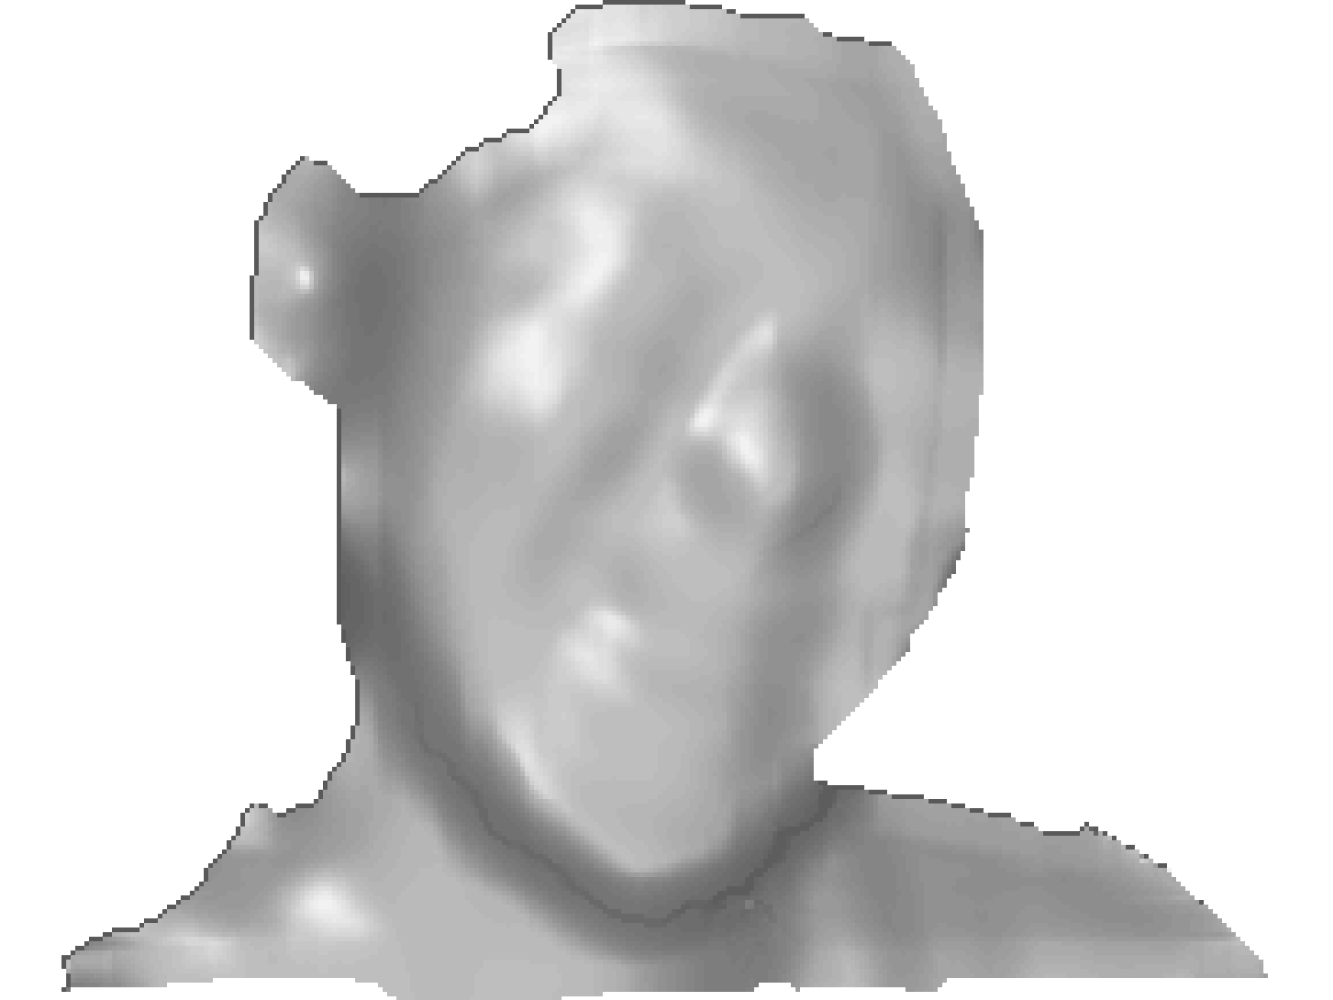
\includegraphics[height = 0.19\linewidth]{figures/methodology/rgbd_face_shape_smooth.pdf} &
   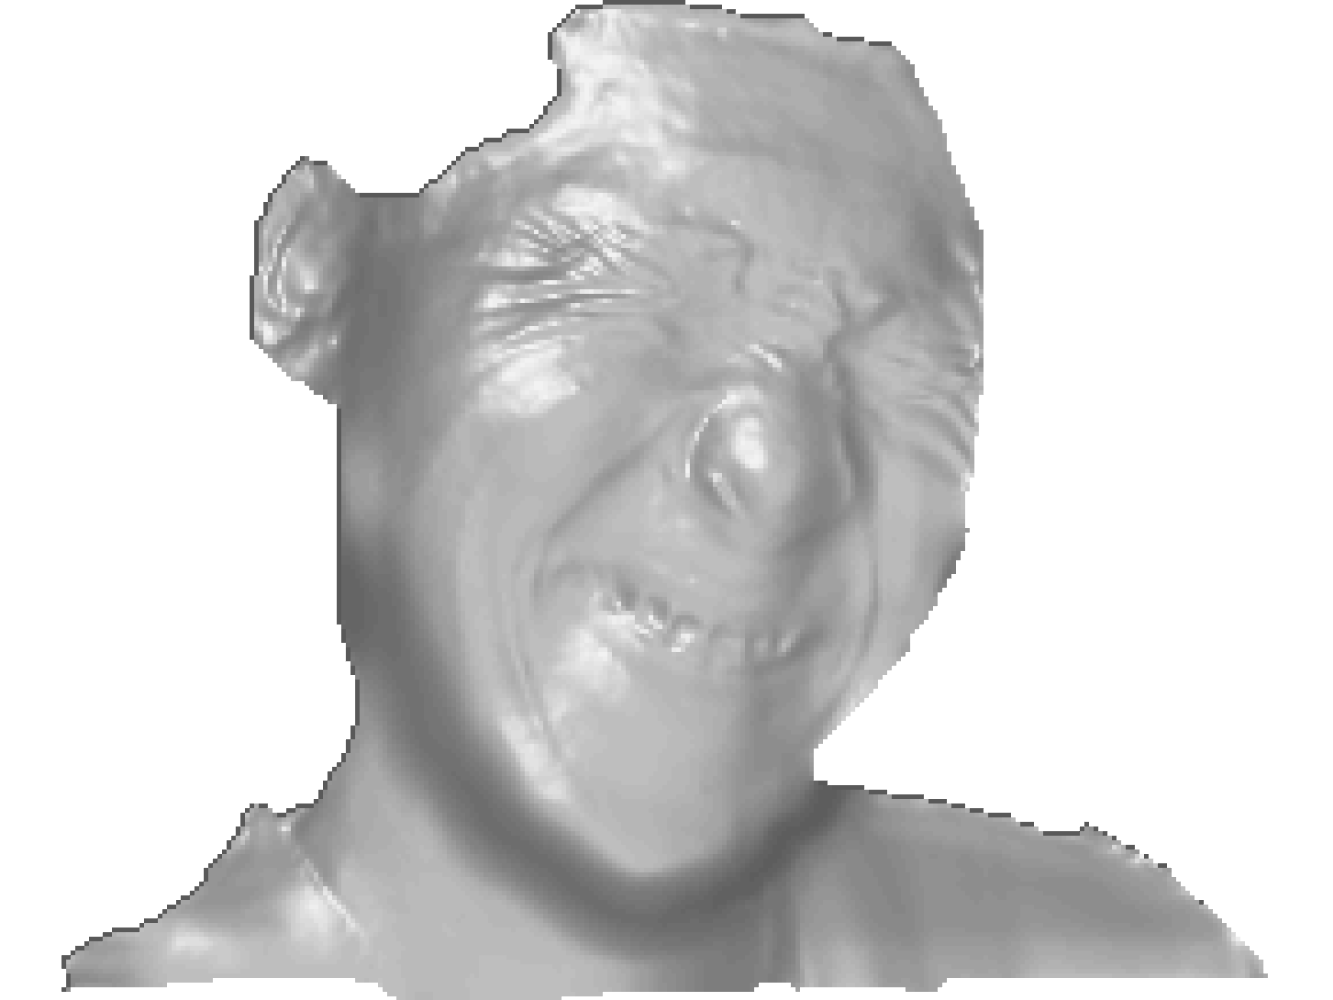
\includegraphics[height = 0.19\linewidth]{figures/methodology/rgbd_face_shape.pdf} \\
   
   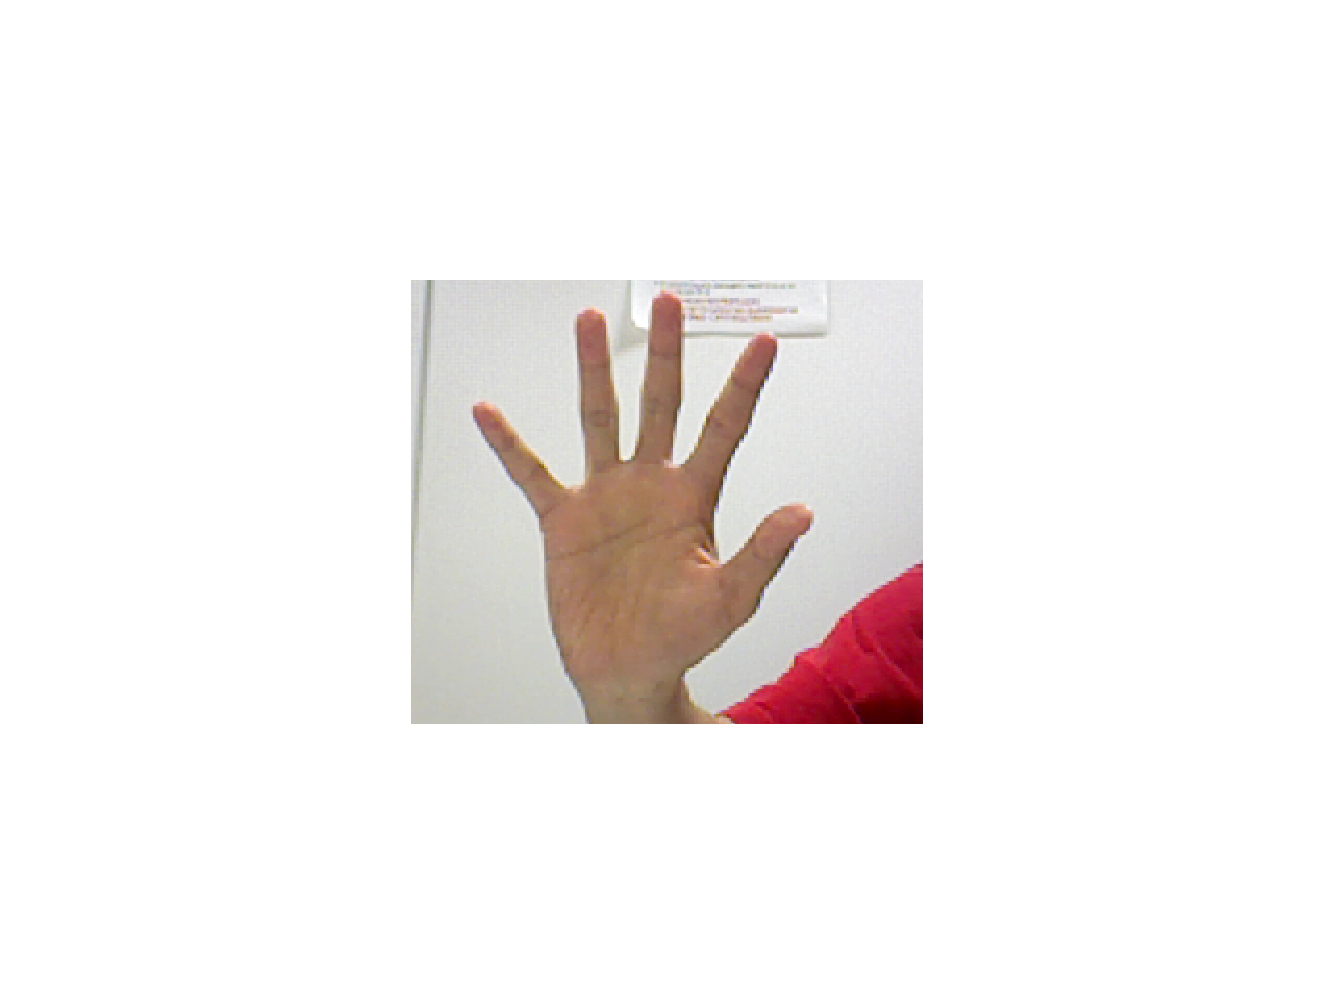
\includegraphics[height = 0.19\linewidth]{figures/methodology/rgbd_palm_rgb.pdf} \hspace{0.05cm}
   &
   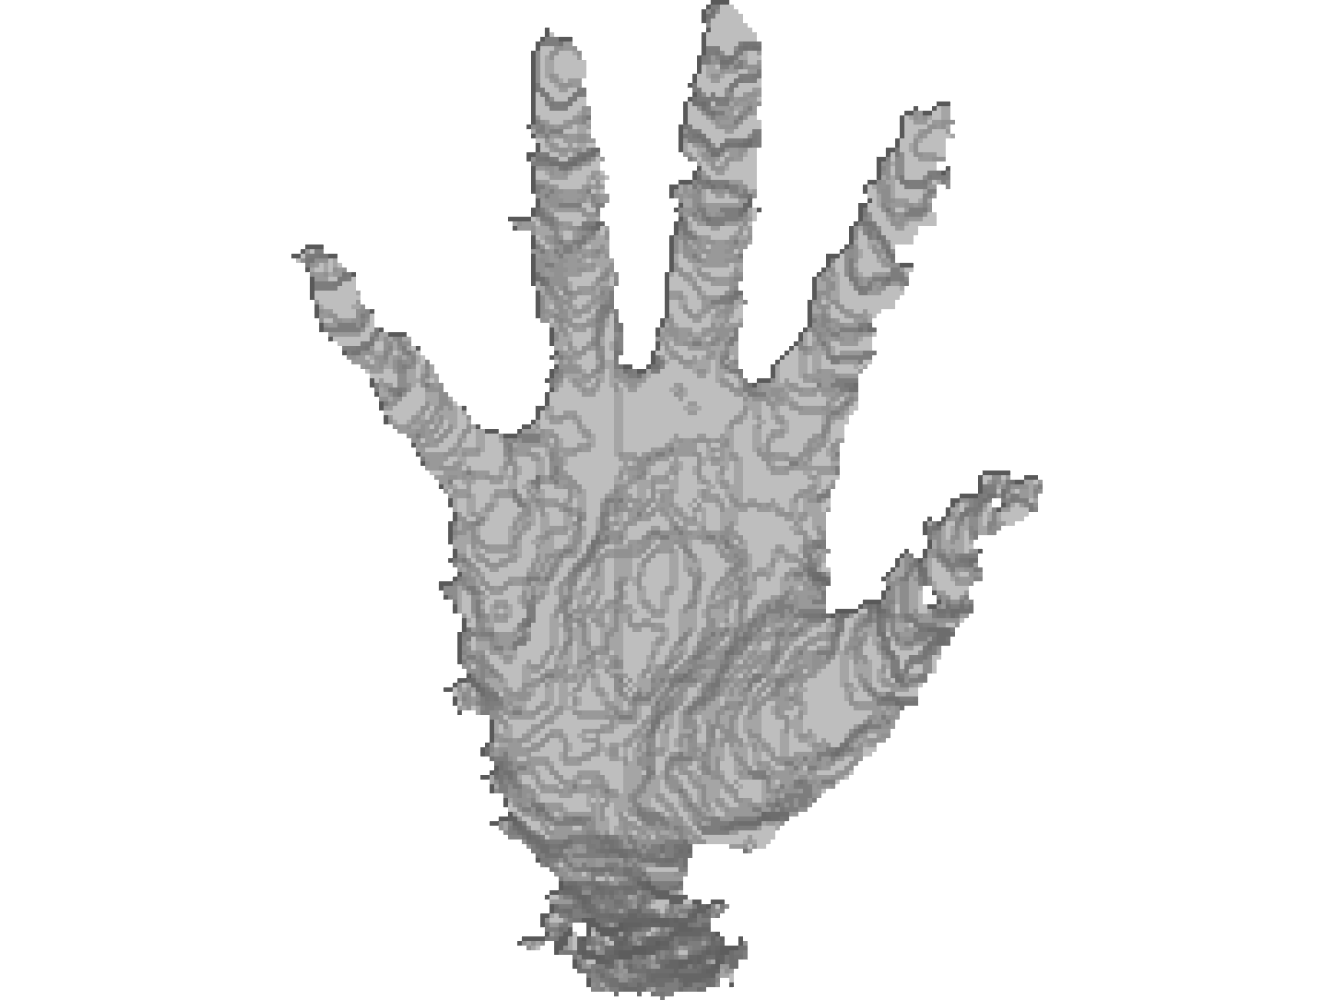
\includegraphics[height = 0.19\linewidth]{figures/methodology/rgbd_palm_shape_init.pdf} &
   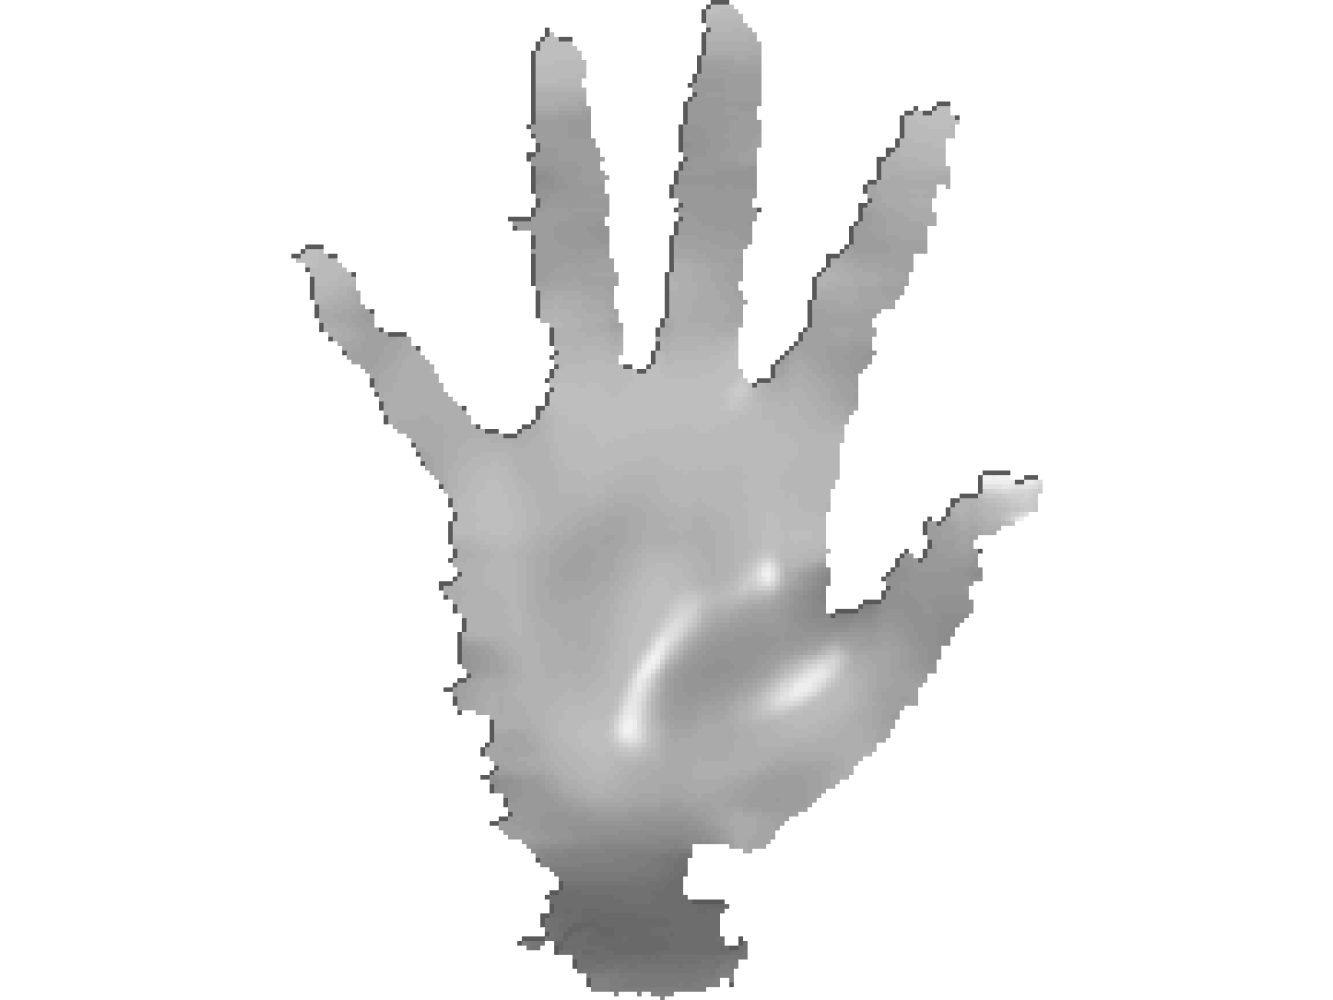
\includegraphics[height = 0.19\linewidth]{figures/methodology/rgbd_palm_shape_smooth.pdf} &
   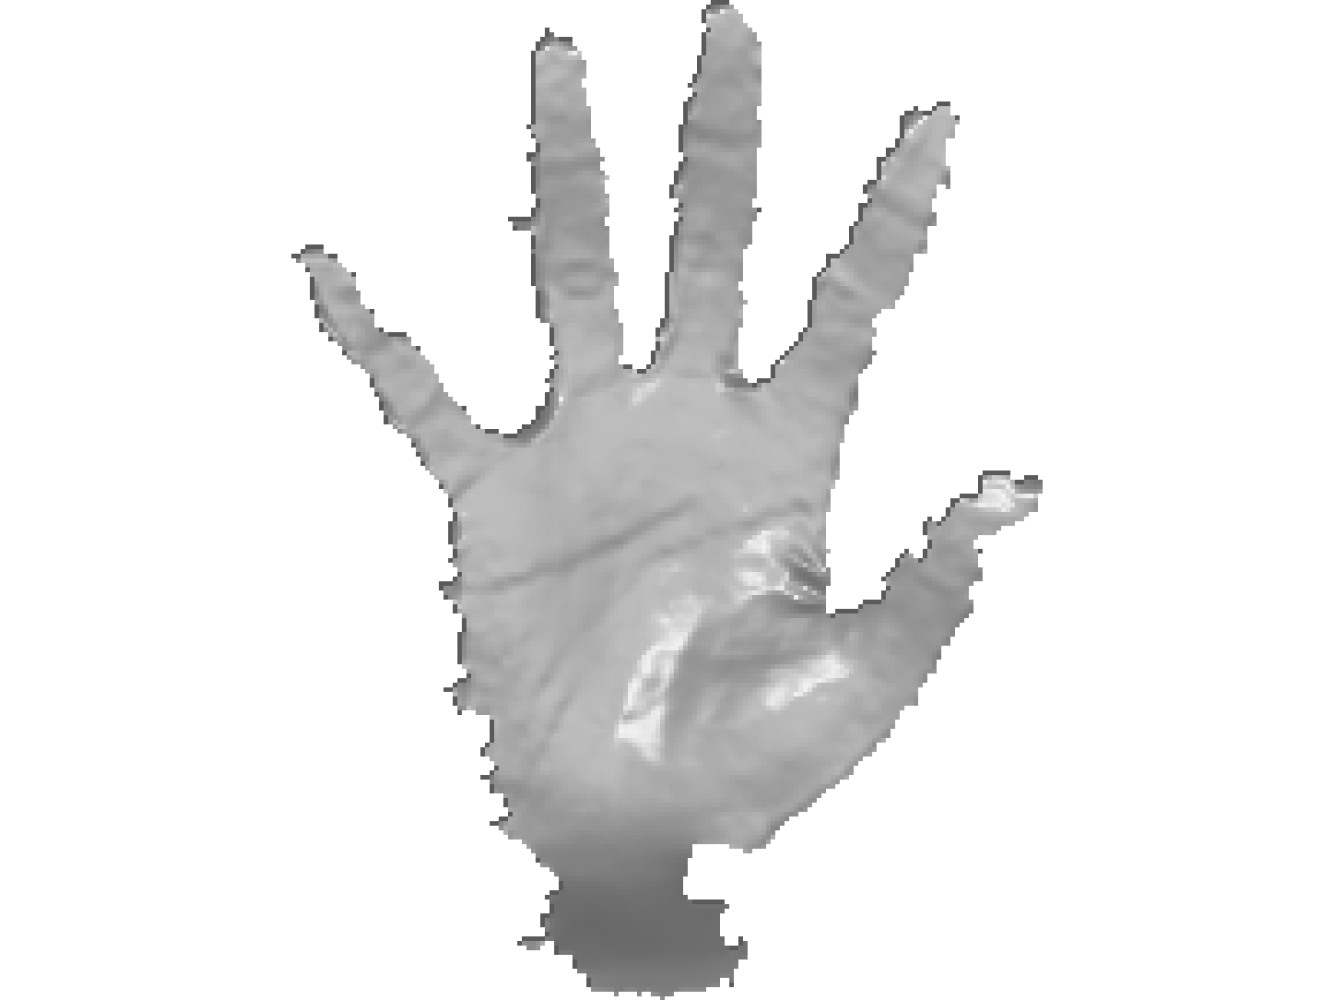
\includegraphics[height = 0.19\linewidth]{figures/methodology/rgbd_palm_shape.pdf} \\
      {RGB image} & {Input depth} & {After pre-processing} &{Refined depth}                 
 \end{tabular}}
\caption{Illustrations for our implementation of RGBD-Fusion Like method. Top row is a T-shirt from~\cite{han2013high}. Middle and bottom row are author's face and palm.  }
\label{fig:rgbd_illustration}
\end{figure}
%&&&&&&&&&&&&&&&&&&&&&&&&&


%----------------------------------------------
\subsection{Limitations}
%----------------------------------------------

Although our RGBD-Fusion like method works moderately well in many real cases, it is not difficult to find the limitations and improve correspondingly.
\begin{itemize}
\item the surface normal modelled by the orthographic projection is merely an ideal case, but it is not really in line with the real world camera model.
And the intrinsic parameters such as the focal length and the coordinate of the principle point are either usually given as a preliminary knowledge, or obtained from calibration without much effort.
Hence, it is reasonable to formulate the surface normal with the perspective projection model.

\item In our RGBD-Fusion like method, only the intensity is applied because the values in RGB channels are more or less the same under the natural scene illumination. 
When we estimated the SH lighting parameters and the albedo in 3 channels separately, the results are quite similar to each other.
So using all three channel rather than just the intensity value will not provide much extra information and improve the depth enhancement. 
Instead, it will just decelerate the whole algorithm.
We ought to find a way to take better advantages of all three channels.

\item The most important inspiration for us to propose RGB ratio model in the next section is, the RGBD-Fusion like method was not convergent in terms of depth enhancement part because of the fix-point method.
In the $4$th line of the Alg.~\ref{alg:rgbd_fusion}, we make the iteration stop when the energy for the depth refinement starts increasing.
This is due to the reason that the fixed-point method actually tries to solve the non-linearity in a tricky way, which is mathematically not totally correct. 
Therefore, we thought of the idea of RGB ratio model, which can eliminate the denominator inside the normal and promise a real linear problem.

\end{itemize}


%%%%%%%%%%%%%%%%%%%%%%%%%%%%%%%%%%%%%%%%%%%%
\section{Proposed method I: RGB Ratio Model}
%%%%%%%%%%%%%%%%%%%%%%%%%%%%%%%%%%%%%%%%%%%%

According to the limitations in the last section, we thought of the idea of RGB ratio model.
First of all, we replace the orthographic projection model with the perspective one.
And then, to fully use the information of the RGB three channels while eliminating the non-linearity in the objective function in the depth refinement, we use the ratio model between every two channels among the three.

It should be noted that we need to add active R, G and B 3 LED lights for the sake of emphasizing the difference among RGB channels.
The green LED is installed in the middle with the red and blue ones on the two sides of ASUS Xtion Pro Live camera (both are around 30 cm to the green LED).
The hardware setup and a color image taken with such setup are illustrated in Fig.~\ref{fig:ratio_setup}.

\begin{figure}[!htbp]
\centering
\subfigure[LED lights setup]{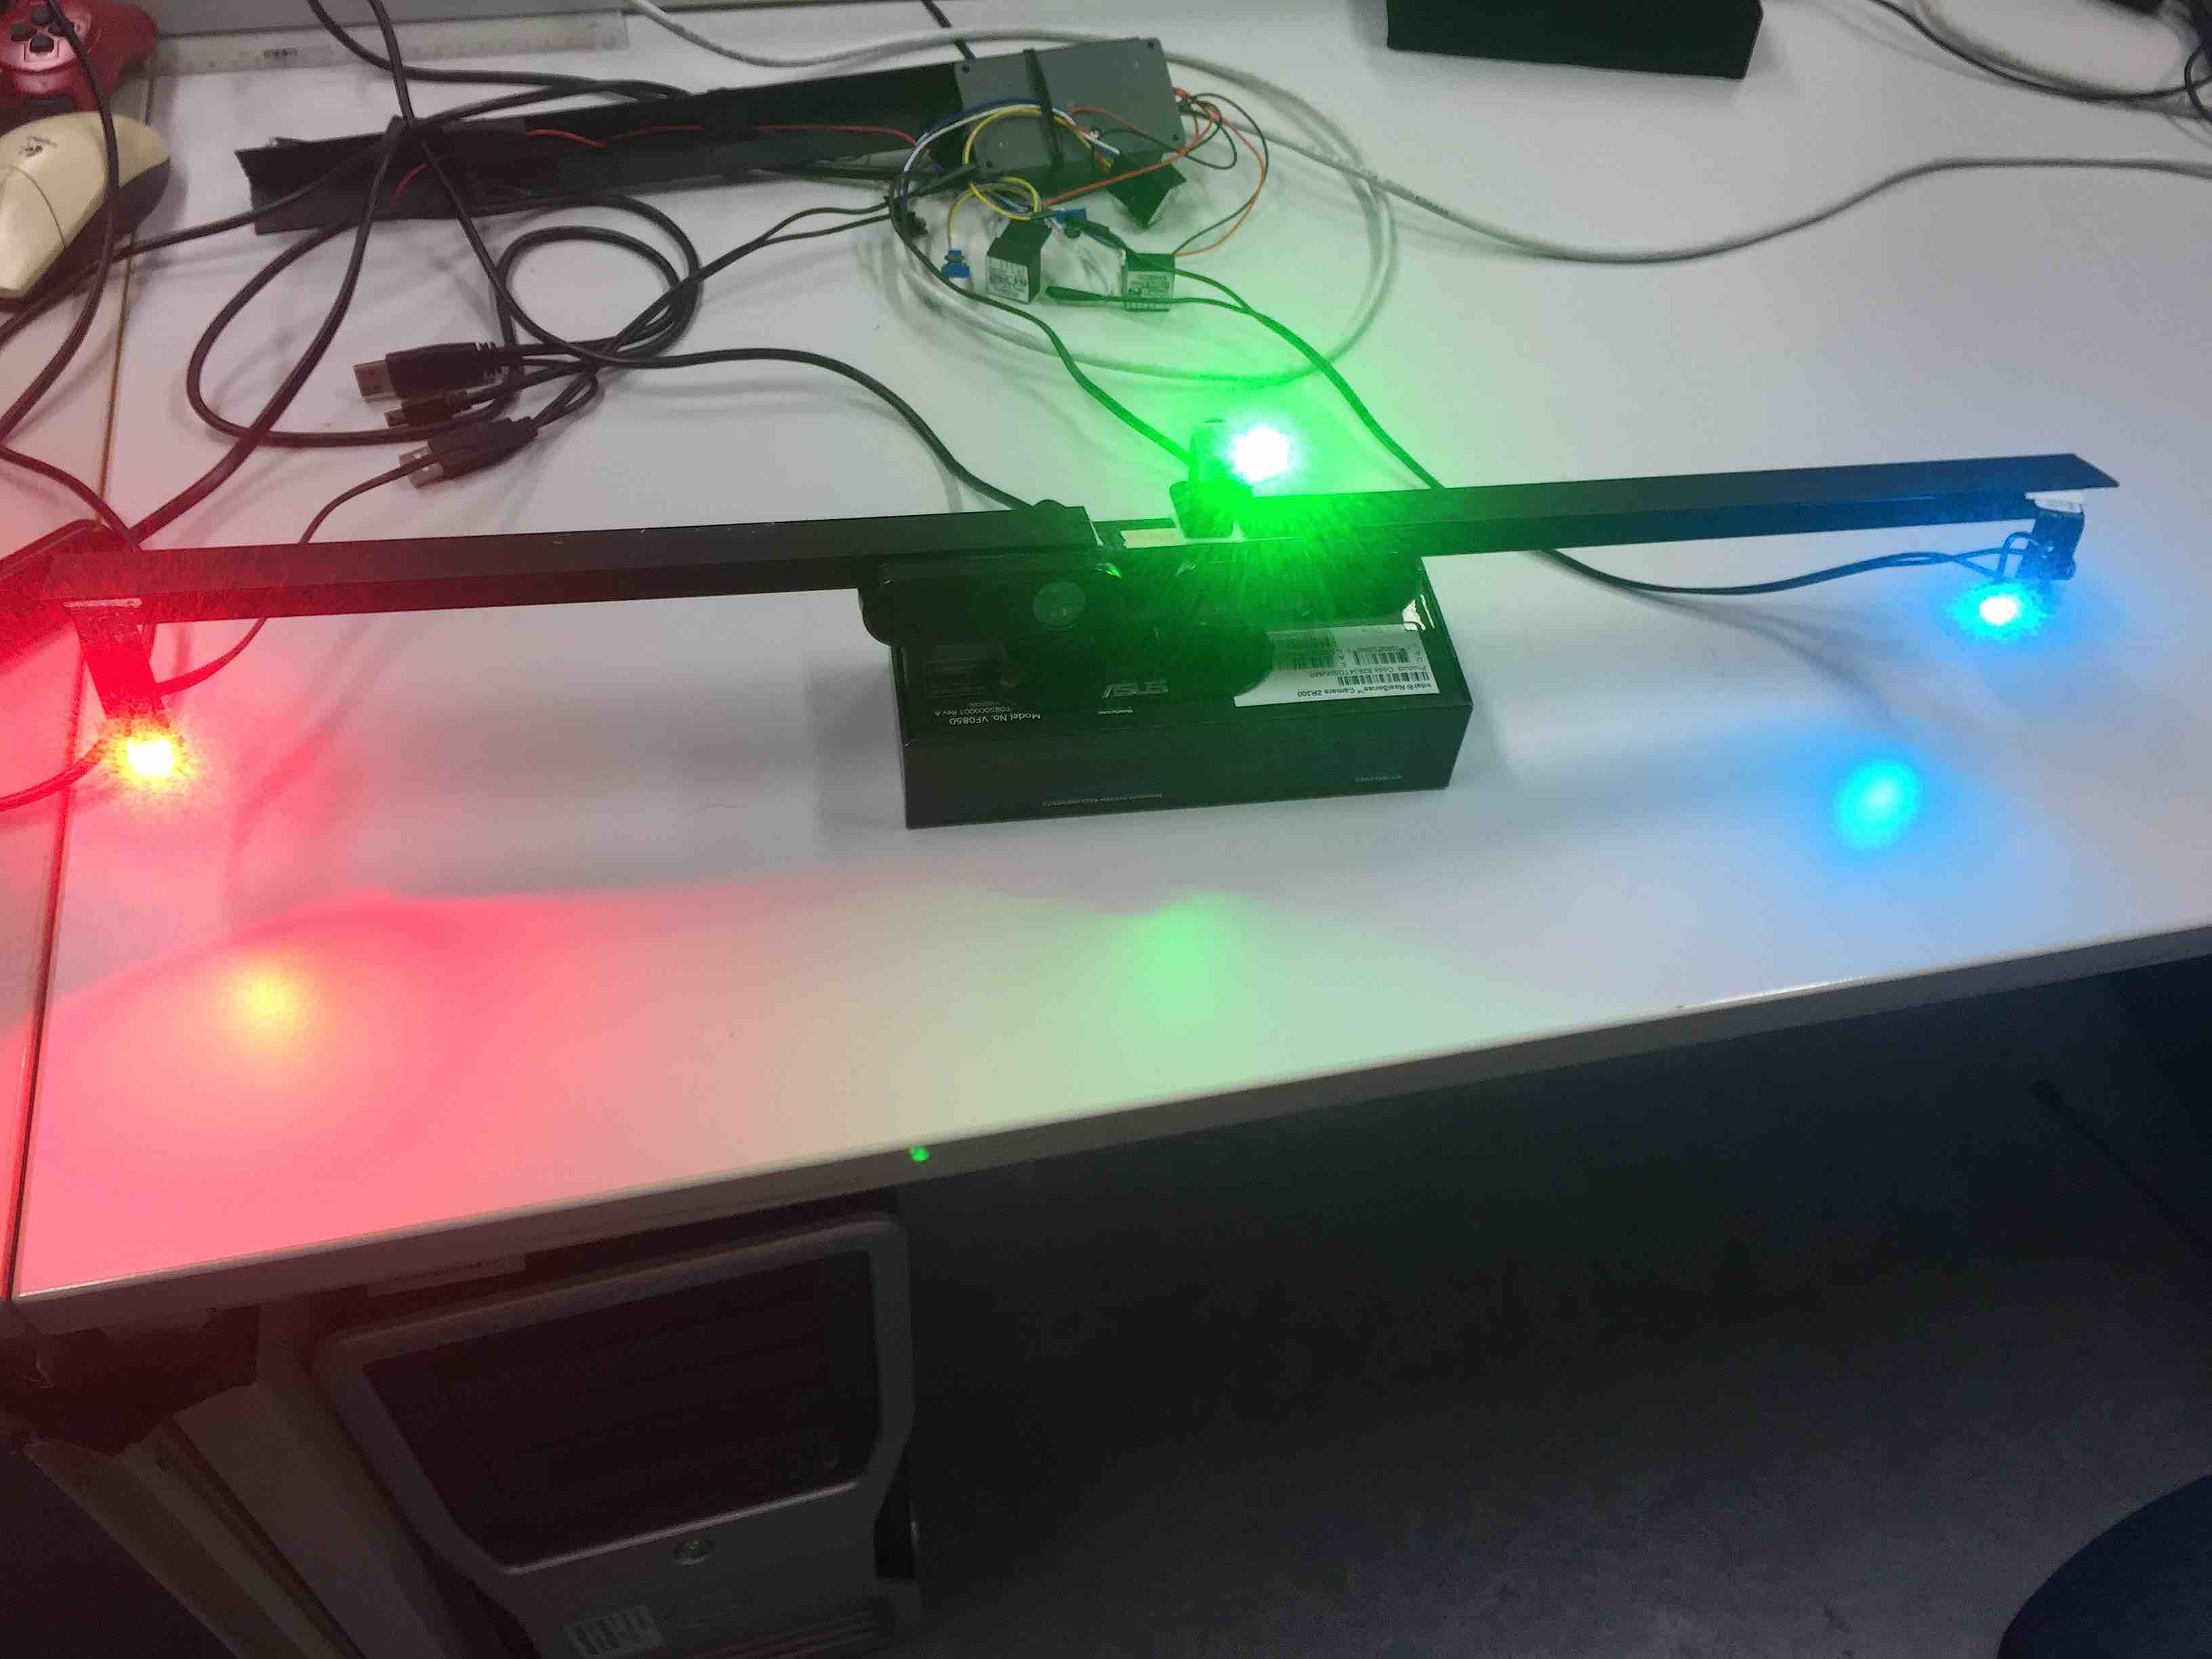
\includegraphics[width=0.45\linewidth]{figures/methodology/ratio_setup.JPG}}
\subfigure[A color image with our lighting setup]{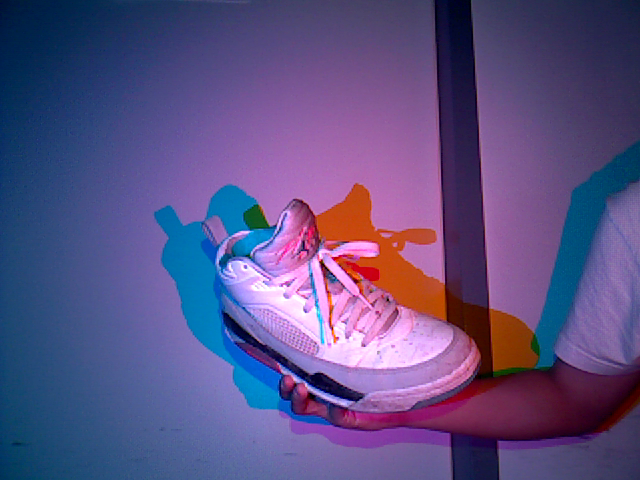
\includegraphics[width=0.45\linewidth]{figures/methodology/ratio_setup_view.png}}
\caption{Illustrations for the RGB LED setup and the corresponding image.}
\label{fig:ratio_setup}
\end{figure}


Now to derive our new ratio model, we treat each channel of the color image $I$ as an single intensity image, denoted by $I_R, I_G, I_B$.
Therefore, 3 equations can be obtained from Eq.~\ref{eq:rgbd_light_model}.

\begin{equation}\label{eq:ratio_prepare}
    \begin{split}
	I_R &= \rho_R(\mathbf{l}_R^\top \mathbf{n} + \varphi_R)\\
	I_G &= \rho_G(\mathbf{l}_G^\top \mathbf{n} + \varphi_G)\\
	I_B &= \rho_B(\mathbf{l}_B^\top \mathbf{n} + \varphi_B)
    \end{split}
\end{equation}

Using R and G channel as an example, we acquire the ratio model:

\begin{equation}\label{eq:ratio_rg_sh1}
%\begin{split}
\frac{I_R - \rho_R \varphi_R}{I_G - \rho_G \varphi_G} = \frac{\rho_R \mathbf{l}_R^\top \mathbf{n}}{\rho_G \mathbf{l}_G^\top \mathbf{n}}
%\rho_G (I_R - \rho_R \varphi_R)\mathbf{l}_G^T \mathbf{n} & = \rho_R (I_G - \rho_G \varphi_G)\mathbf{l}_R^T\mathbf{n}\\
%\end{split}
\end{equation}

Similarly, we can acquire another two ratio models which are between green and blue, and blue and red channels respectively.
We are able to notice from Eq~\ref{eq:ratio_rg_sh1} that, the non-linearity problem mentioned before has been solved because the denominator in the surface normal $\mathbf{n}$ is cancelled out.
Also, our normal is derived from perspective camera model and can be represented as a function of $\; \log z$. 
For the sake of simplicity we directly represent $z = \log z$ and redefine $\mathbf{n}$ without the normalizer in the following part.
%$$$$$$$$$$$$$$$$
\begin{equation}\label{eq:ratio_normal}
    \mathbf{n}(x,y) =
     \begin{pmatrix}
         fz_x(x,y)\\
         fz_y(x,y)\\
         -1 - \tilde{x}z_x(x,y) - \tilde{y}z_y(x,y)
     \end{pmatrix}
\end{equation}
%$$$$$$$$$$$$$$$$
where $f$ is the focal length, $(\tilde{x}, \tilde{y}) = (x- x_0, y - y_0)$, with $(x_0, y_0)$ the coordinates of principle points and $(x,y)$ the coordinate of a pixel inside the given mask, $[z_x, z_y]$ is the gradient of depth $z$.

The overall energy for the proposed RGB ratio model method is:
\begin{equation}\label{eq:ratio_energy}
    \begin{split}
	E(\mathcal{P}^{(t)}, z^{(t)}, \mathbf{s}^{(t)}) = \; &\lVert Ratio(\mathcal{P}^{(t)}, z^{(t)}) \rVert^2_2 
	+ \lambda_z||z^{(t)} - z_0||^2 \\&
	+ \lambda_{\rho}^1 \lVert \omega \nabla \mathcal{P}^{(t)} \rVert^2  
	+ \lambda_{\rho}^2 \lVert \mathcal{P} - \mathcal{P}^{(t-1)}\rVert^2 
	+ \sum_{c} \lVert \rho_c \; \mathbf{s}_c^\top \tilde{\mathbf{n}} - I_c \rVert^2_2, \; c\in\{R,G,B\}
    \end{split}
\end{equation}
where $\mathcal{P}$ is the stack of RGB albedo.
This energy is composed of a proposed ratio SFS term, a depth fidelity term, an albedo smoothness term, an albedo fidelity term and a SH estimation term.
Now we will explain our proposed algorithm based on the new ratio model.

%The key to this ratio model is toenlarge the difference of pixel values, light directions and the albedo in 3 channels

%----------------------------------------------
\subsection{Algorithm details}
%----------------------------------------------
Similar to the RGBD-Fusion Like method, the algorithm is separated to 3 parts: light estimation, albedo estimation and depth enhancement.
However, our new method requires an initial estimation of the color albedo as the input of our iterative method, and hence, we calculate the initial SH parameters $\mathbf{l}^{0}$ with Eq.~\ref{eq:rgbd_light_model} and the color albedo $\mathcal{P}^{0}$ with Eq.~\ref{eq:rgbd_albedo_estimate} using the old model.
Noted that the initial estimation is performed with respect to all RGB three channels.

\textbf{Albedo refinement:}
with the acquired $\rho^{0}$ and $\mathbf{l}^{0}$, we can start the iteratively refinement process.
In order to refine the color albedo with our ratio model, in each iteration, we need to reshape the ratio model described in Eq.~\ref{eq:ratio_rg_sh1} as follows:
\begin{equation}\label{eq:ratio_albedo_prepare}
\begin{split}
I_G \mathbf{l}_R^\top\mathbf{n} \rho_R - I_R \mathbf{l}_G^\top\mathbf{n} \rho_G  = \rho_R \rho_G (\varphi_G\mathbf{l}_R^\top \mathbf{n} - \varphi_R\mathbf{l}_G^\top \mathbf{n})\\
I_B \mathbf{l}_G^\top\mathbf{n} \rho_G - I_G \mathbf{l}_B^\top\mathbf{n} \rho_B  = \rho_G \rho_B (\varphi_B\mathbf{l}_G^\top \mathbf{n} - \varphi_G\mathbf{l}_B^\top \mathbf{n})\\
I_R \mathbf{l}_B^\top\mathbf{n} \rho_B - I_B \mathbf{l}_R^\top\mathbf{n} \rho_R  = \rho_B \rho_R (\varphi_R\mathbf{l}_B^\top \mathbf{n} - \varphi_B\mathbf{l}_R^\top \mathbf{n})
\end{split}
\end{equation}
For each pixel, we can reformulate the Eq.~\ref{eq:ratio_albedo_prepare} to a matrix form:
%$$$$$$$$$$$$$$$$
\begin{equation}\label{eq:rho_matrix}
    \begin{pmatrix}
        I_G \mathbf{l}_R^\top\mathbf{n} & - I_R \mathbf{l}_G^\top\mathbf{n} & 0 \\
        0 & I_B \mathbf{l}_G^\top\mathbf{n} & - I_G \mathbf{l}_B^\top\mathbf{n} \\
        - I_B \mathbf{l}_R^\top\mathbf{n} & 0 & I_R \mathbf{l}_B^\top\mathbf{n} 
    \end{pmatrix}
    \begin{pmatrix}
        \rho_R(x,y)\\
        \rho_G(x,y)\\
        \rho_B(x,y)
     \end{pmatrix}_{3 \times 1}
    =
    \begin{pmatrix}
        \rho_R \rho_G (\varphi_G\mathbf{l}_R^\top \mathbf{n} - \varphi_R\mathbf{l}_G^\top \mathbf{n})\\
        \rho_G \rho_B (\varphi_B\mathbf{l}_G^\top \mathbf{n} - \varphi_G\mathbf{l}_B^\top \mathbf{n})\\
        \rho_B \rho_R (\varphi_R\mathbf{l}_B^\top \mathbf{n} - \varphi_B\mathbf{l}_R^\top \mathbf{n})
    \end{pmatrix}
\end{equation}
This small linear system can be generalized to a big sparse linear system denoted as $\mathbf{A}_{\rho}\cdot {\mathcal{P}} = \mathbf{b}_{\rho}$.
The structure of this equation can be found in Appendix~\ref{appendix:implement}.
Here, $\mathcal{P}$ represents the stack of RGB three albedos.
%$$$$$$$$$$$$$$$$

To acquire the RGB albedos, some regularization terms are required similar to Eq.~\ref{eq:rgbd_albedo_estimate}. Now in each iteration, we fix the normal and the SH parameters, the minimization problem of color albedo in Eq.~\ref{eq:ratio_energy} in each iteration now becomes:
%$$$$$$$$$$$$$$$$
\begin{equation}\label{eq:ratio_albedo_refine}
    \mathcal{P}^{(t)} = 
    \argmin_{\mathcal{P}} \lVert\mathbf{A}_{\rho}^{(t-1)}\mathcal{P} - \mathbf{b}_{\rho}^{(t-1)}\rVert^2 
    + \lambda_{\rho}^1 \lVert \omega \nabla \mathcal{P} \rVert^2  
    + \lambda_{\rho}^2 \lVert \mathcal{P} - \mathcal{P}^{(t-1)}\rVert^2
\end{equation}
where the weight $\omega = \begin{pmatrix} \omega_R\\ \omega_G\\ \omega_B \end{pmatrix}$, which can be denoted as:
\begin{equation}
\omega_c = \exp(- \frac{\sigma_c ||\nabla I_c||^2}{\max ||\nabla I_c||^2}), \quad c \in \{R,G,B\}
\end{equation}
$\sigma_c$ is a tuning parameter for each channel $c$.  
We can notice from Fig.~\ref{fig:ratio_albedo_demo} the importance of imposing the weight $\omega$.
Without the weight, the isotropic smoothness regularization will not take care of the boundary of the albedo, which leads to the bad depth enhancement.
%$$$$$$$$$$$$$$$$

\begin{figure}[!ht]
\centering
\setlength{\tabcolsep}{0.1em} % column spacing
 {\renewcommand{\arraystretch}{0.6}% row spacing
\begin{tabular}{c|c c c}
   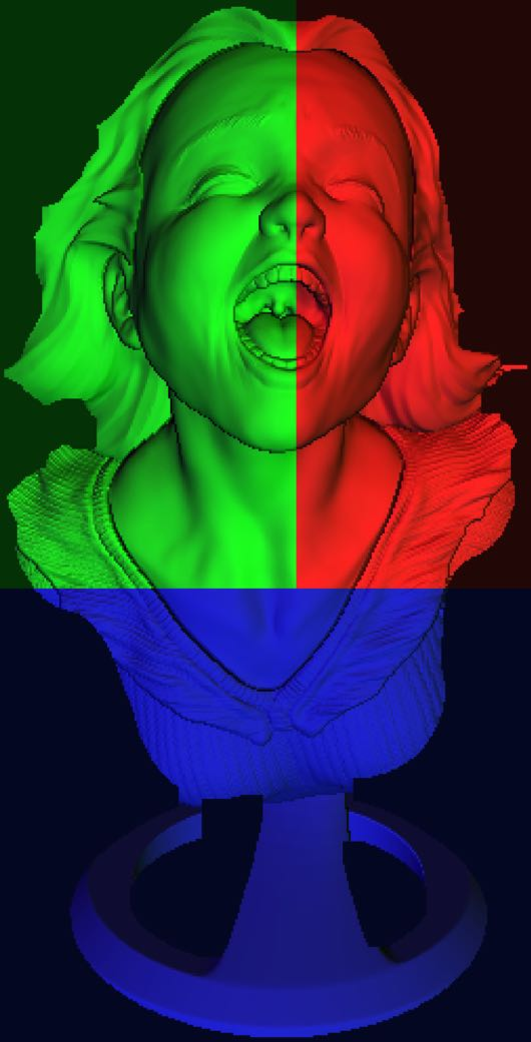
\includegraphics[height = 0.32\linewidth]{figures/methodology/ratio_syn_rgb.pdf} \hspace{0.1em}
   &\hspace{0.1em}
   
\includegraphics[height = 0.32\linewidth]{figures/methodology/ratio_syn_albedoGT.pdf} &
   
\includegraphics[height = 0.32\linewidth]{figures/methodology/ratio_syn_albedoNR.pdf} &
   
\includegraphics[height = 0.32\linewidth]{figures/methodology/ratio_syn_albedoR.pdf} \\
   
   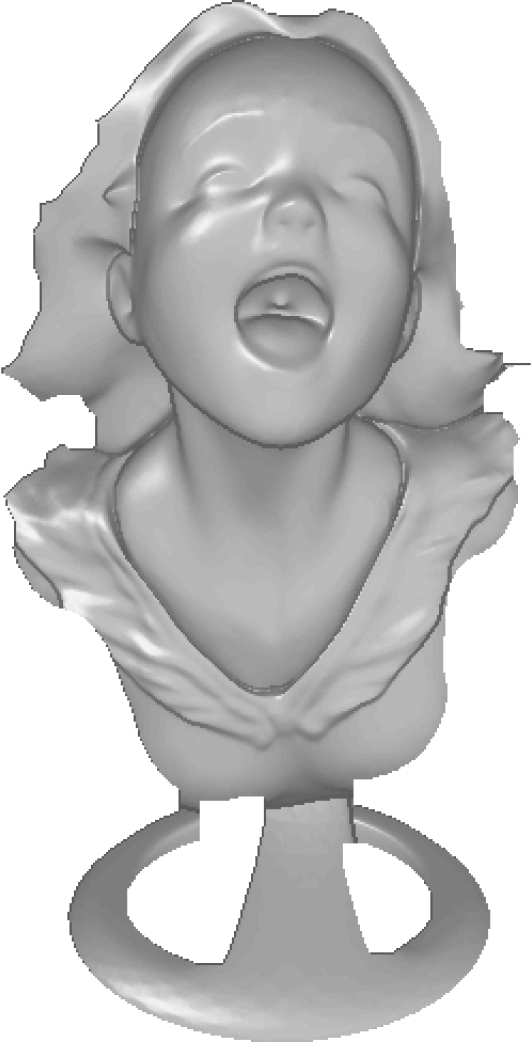
\includegraphics[height = 0.32\linewidth]{figures/methodology/ratio_syn_shapeInput.pdf} \hspace{0.1em}
   &\hspace{0.1em}
   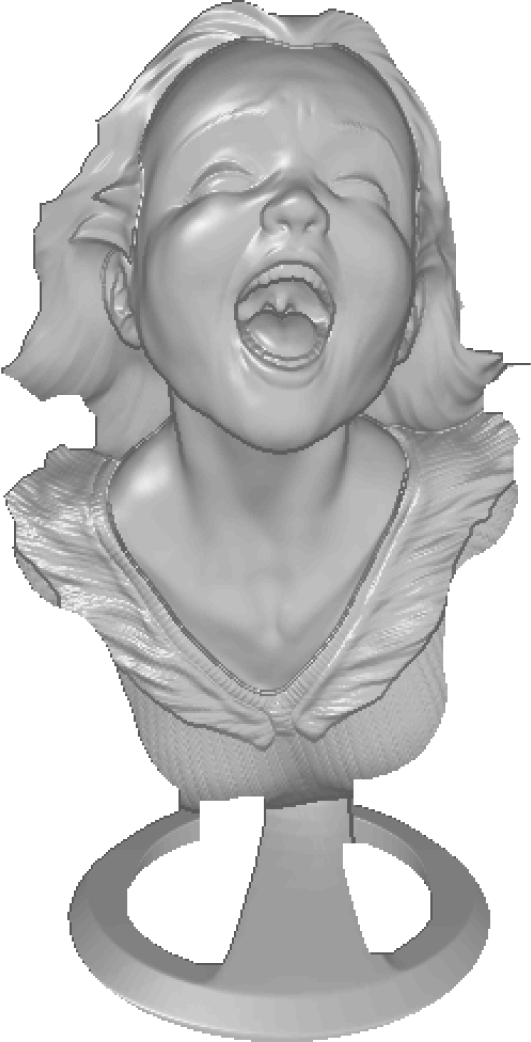
\includegraphics[height = 0.32\linewidth]{figures/methodology/ratio_syn_shapeGT.pdf} &
   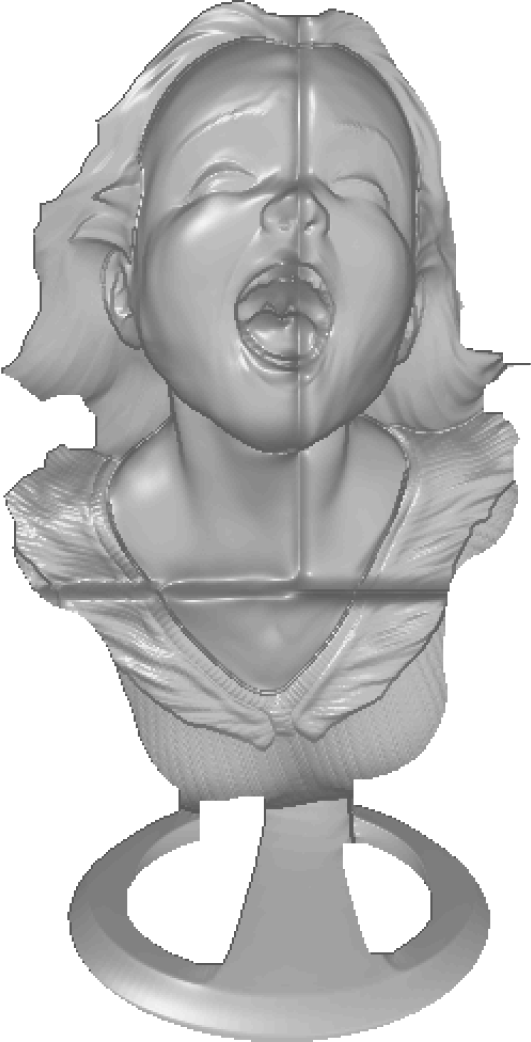
\includegraphics[height = 0.32\linewidth]{figures/methodology/ratio_syn_shapeNR.pdf} &
   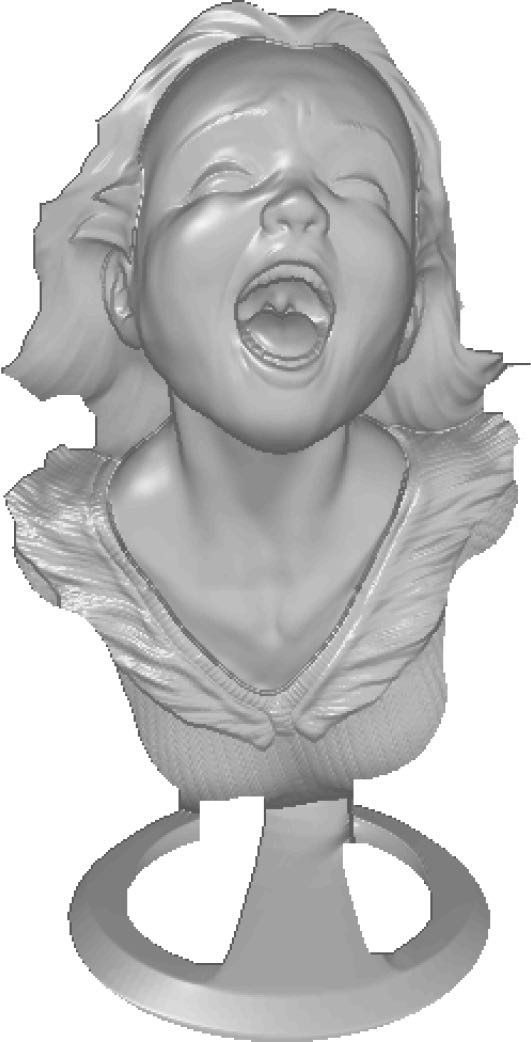
\includegraphics[height = 0.32\linewidth]{figures/methodology/ratio_syn_shapeR.pdf} \\
   {Input} & {Ground truth} & {No weight} &{With weight}                 
 \end{tabular}}
\caption{Illustrations for the importance of the weight $\omega$ inside regularization term in Eq.~\ref{eq:ratio_albedo_refine} when estimating the albedo. Top: first one is the input color image and the rest three are the albedos. Bottom: 3D shape from depth. Noted that the light parameter is given.}
\label{fig:ratio_albedo_demo}
\end{figure}


There are three interesting aspects about the albedo estimation which worth having a few more words:
\begin{enumerate}
    \item One observation about Eq.~\ref{eq:rho_matrix} is that, if the SH parameters are the same among the three channels, the right side of the equal sign is or close to 0. 
    This is the reason why we need to set up 3 LED lights with a distance to each other, which will provide us enough difference on the light directions.
    \item Instead of using anisotropic Laplacian regularization in RGBD-Like method, the smoothness term in Eq.~\ref{eq:ratio_albedo_refine} only takes the use of the gradient of $\rho$ with a weight only depending on the RGB image's gradient.
    It takes less efforts to build such a smoothness term than the anisotropic term, but the acquired albedo is still satisfying.
    \item If we don't use a data fidelity term $\lVert \mathcal{P} - \mathcal{P}^{(t-1)}\rVert^2$, the albedo will get increasingly dark after several iterations. 
    This is due to the fact that there also exist the RGB albedos in $\mathbf{b}_{\rho}$, so $\rho = 0$ will become the solution of our ratio model term.
    Therefore, adding the data term can not only avoid such problem, but help refine the albedo iteratively. 
\end{enumerate}

\textbf{Depth refinement}:
After acquiring the color albedo in time step $t$, we are going to refine the depth with the help of the ratio model.
First we reshape Eq.~\ref{eq:ratio_rg_sh1} with the surface normal $\mathbf{n}$ as the argument:
%$$$$$$$$$$$$$$$$
\begin{equation}\label{eq:ratio_depth1}
\begin{split}
\rho_G (I_R - \rho_R \varphi_R)\mathbf{l}_G^T \mathbf{n} - \rho_R (I_G - \rho_G \varphi_G)\mathbf{l}_R^T\mathbf{n} = 0\\
\rho_B (I_G - \rho_G \varphi_G)\mathbf{l}_B^T \mathbf{n} - \rho_G (I_B - \rho_B \varphi_B)\mathbf{l}_G^T\mathbf{n} = 0\\
\rho_R (I_B - \rho_B \varphi_B)\mathbf{l}_R^T \mathbf{n} - \rho_B (I_R - \rho_R \varphi_R)\mathbf{l}_B^T\mathbf{n} = 0 
\end{split}
\end{equation}
since the normal $\mathbf{n}$ now is a function of $z$, Eq.~\ref{eq:ratio_depth1} can be actually simplified as below (the derivation details can be found in Appendix~\ref{appendix:implement}):
\begin{equation}
    \Psi z = 0
\end{equation}
When the estimated color albedo and light are fixed, the depth refinement problem in Eq.~\ref{eq:ratio_energy} is:

\begin{equation}\label{eq:ratio_depth_refine}
    z^{(t)}= \argmin_{z}  ||\Psi z||^2 + \lambda_z||z - z_0||^2
\end{equation}

\textbf{Light estimation}
Since estimating light with the proposed ratio model is a ill-posed problem, we decided to use Eq.~\ref{eq:rgbd_light_estimate} to calculate the SH parameters for each channel when the albedo and the surface normal are freezed. The minimization problem from Eq.~\ref{eq:ratio_energy} can then be written as:
\begin{equation}\label{eq:ratio_light_estimate}
    \mathbf{s}^{(t)} = \argmin_{\mathbf{s} = (\mathbf{s}_R, \mathbf{s}_G, \mathbf{s}_B)}\sum_{c} \lVert \rho_c \; \mathbf{s}_c^\top \tilde{\mathbf{n}} - I_c\rVert^2_2, \; c\in\{R,G,B\}
\end{equation}

\begin{algorithm}[!htbp]
	\begin{algorithmic}[1]
  		\caption{\textbf{RGB Ratio Model method}}
		\label{alg:rgb_ratio}
		 \renewcommand{\algorithmicrequire}{\textbf{Input:}}
		 \renewcommand{\algorithmicensure}{\textbf{Output:}}
		 \REQUIRE Initial depth image $z_0$, RGB image $I$, mask, focal length, principle point
		 \vspace{1.8mm}
		 \STATE $\mathbf{s}^{(0)} = \argmin \limits_{\mathbf{s}} E(\mathcal{P} =1, z_0)$ \COMMENT{Eq.~\ref{eq:ratio_light_estimate}}
		 \STATE Estimate initial color albedo and build $\mathcal{P}^{(0)}$  \COMMENT{Eq.~\ref{eq:rgbd_albedo_estimate}}
		 \STATE t = 1, $z^{(0)} = z_0$
		 \vspace{1.8mm}
		  \WHILE {$ \frac{\Vert E(\mathcal{P}^{(t)}, z^{(t)}, \mathbf{s}^{(t)}) - E(\mathcal{P}^{(t-1)}, z^{(t-1)}, \mathbf{s}^{(t-1)})\Vert}{E(\mathcal{P}^{(t-1)}, z^{(t-1)}, \mathbf{s}^{(t-1)})} > \epsilon$}
		   \vspace{1.8mm}
			\STATE $\mathcal{P}^{(t)} = \argmin \limits_{\mathcal{P}} E(\mathcal{P}^{(t-1)}, z^{(t-1)}, \mathbf{s}^{(t-1)})$ \COMMENT{Eq.~\ref{eq:ratio_albedo_refine}}
			  \STATE $z^{(t)} = \argmin \limits_{z} E(\mathcal{P}^{(t)}, \mathbf{s}^{(t-1)})$ \COMMENT{Eq.~\ref{eq:ratio_depth_refine}}
			  \STATE $\mathbf{s}^{(t)} = \argmin \limits_{\mathbf{s}} E(\mathcal{P}^{(t)}, z^{(t)})$ \COMMENT{Eq.~\ref{eq:ratio_light_estimate}}
			  \vspace{1.8mm}
		          \STATE $t := t + 1$
		 \vspace{1.8mm}
		  \ENDWHILE
		  \ENSURE  Refined depth image $z^{(t)}$ and stacked color albedo $\mathcal{P}^{(t)}$
	\end{algorithmic}
\end{algorithm}

%&&&&&&&&&&&&&&&&&&&&&&&&&
\begin{figure}[!ht]
\centering
\setlength{\tabcolsep}{0.1em} % column spacing
 {\renewcommand{\arraystretch}{0.6}% row spacing
\begin{tabular}{c|c c c}
   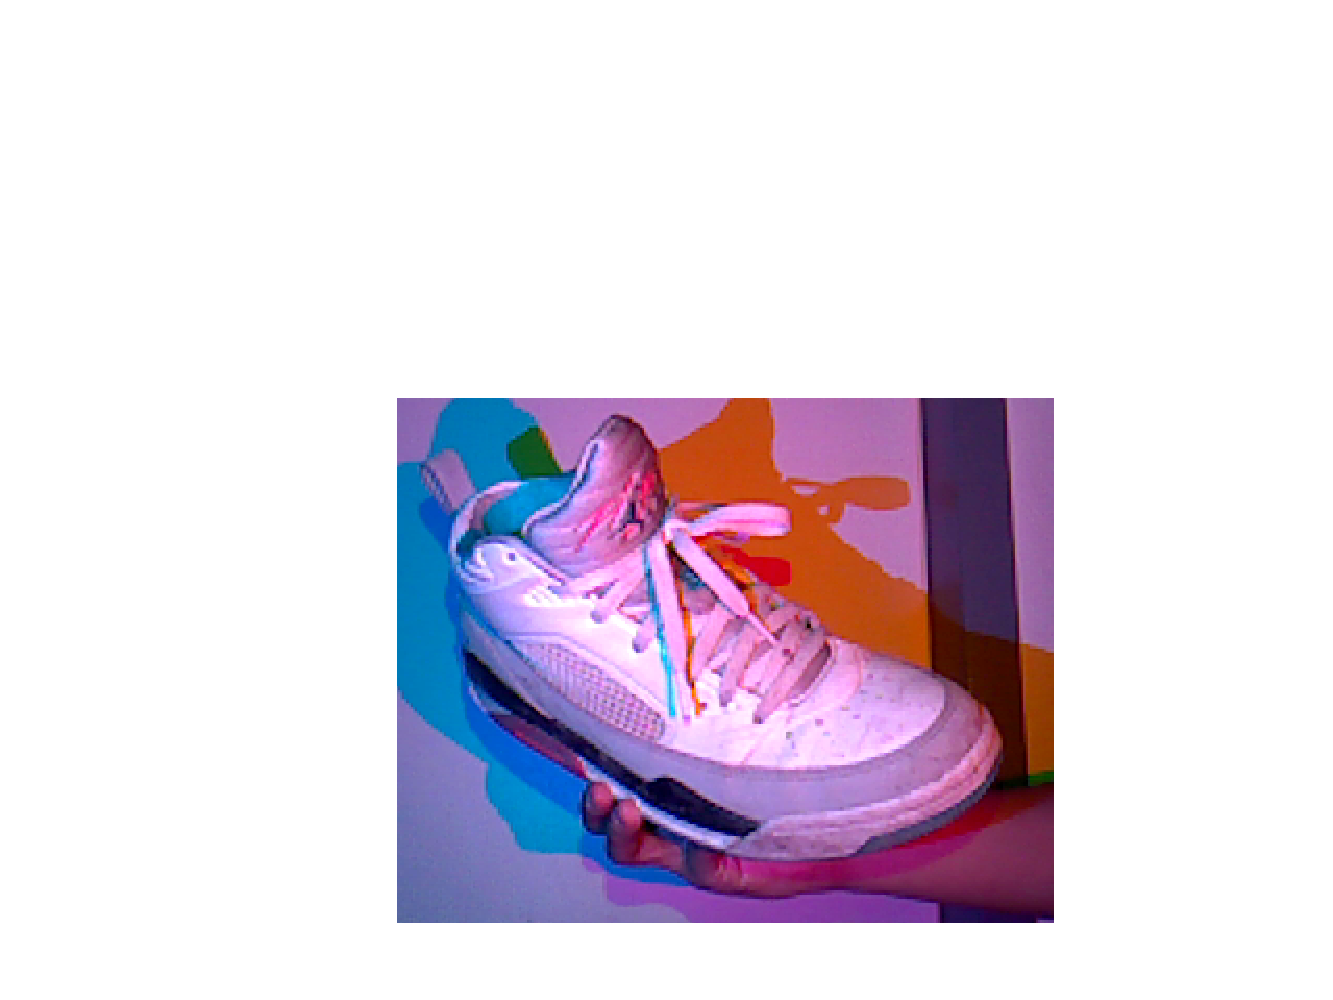
\includegraphics[height = 0.19\linewidth]{figures/methodology/ratio_shoe_rgb.pdf} 
   &
   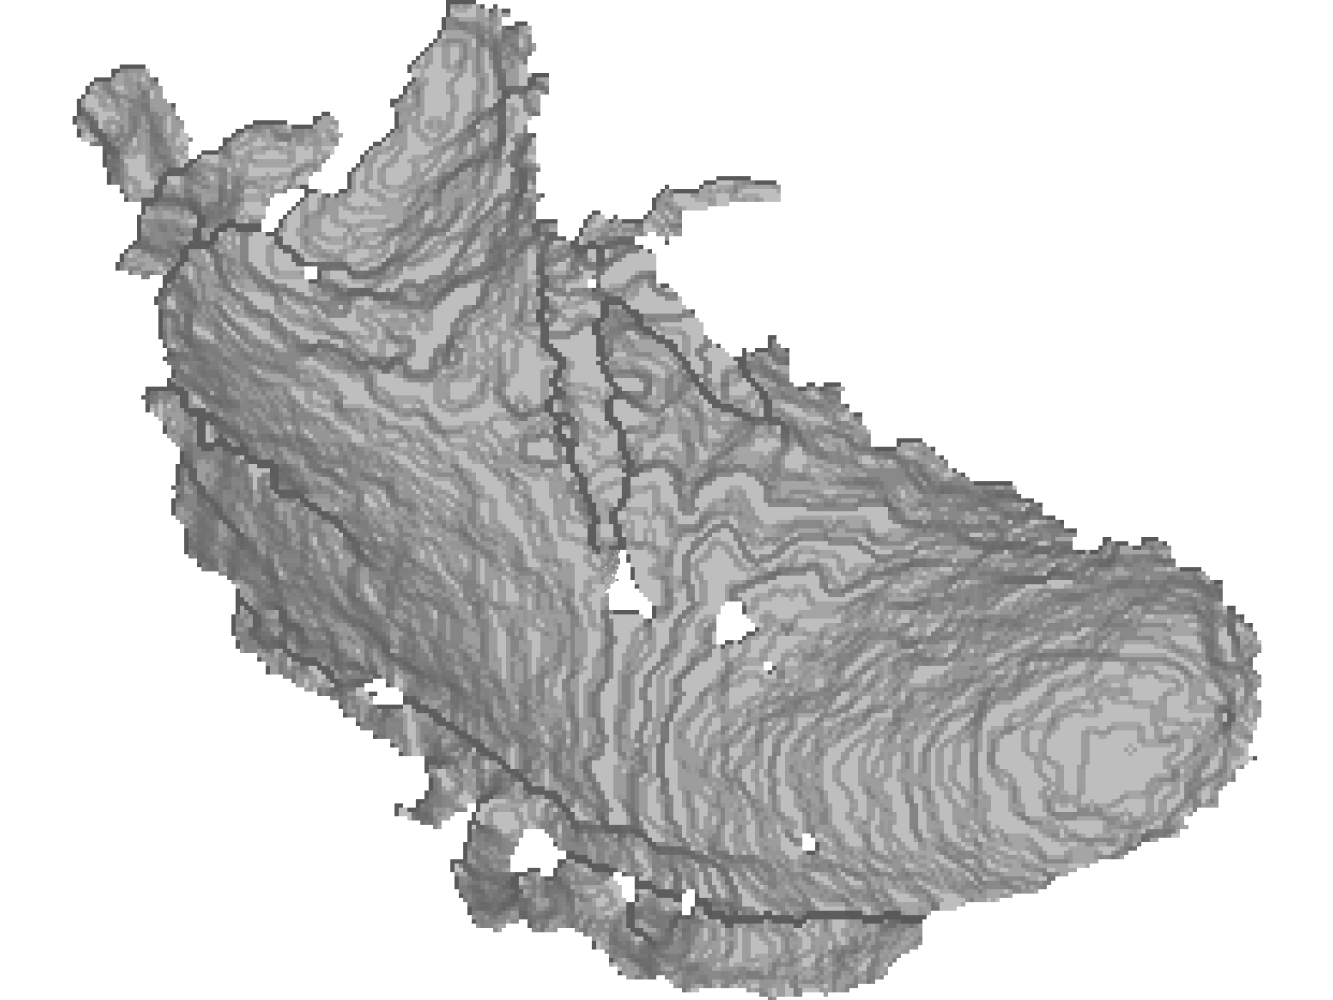
\includegraphics[height = 0.19\linewidth]{figures/methodology/ratio_shoe_shape_init.pdf} &
   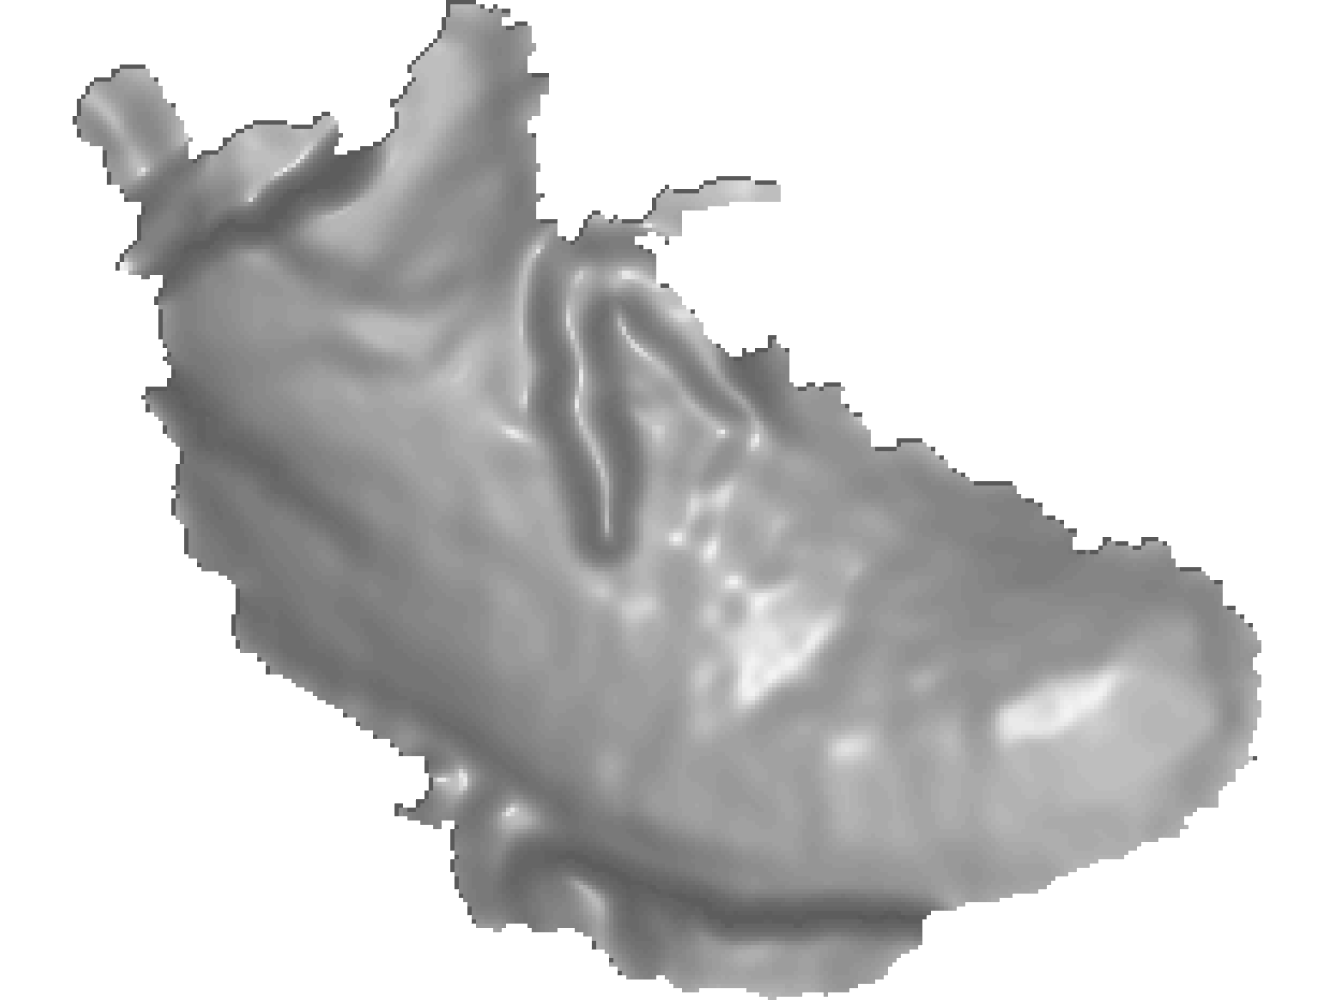
\includegraphics[height = 0.19\linewidth]{figures/methodology/ratio_shoe_shape_smooth.pdf} &
   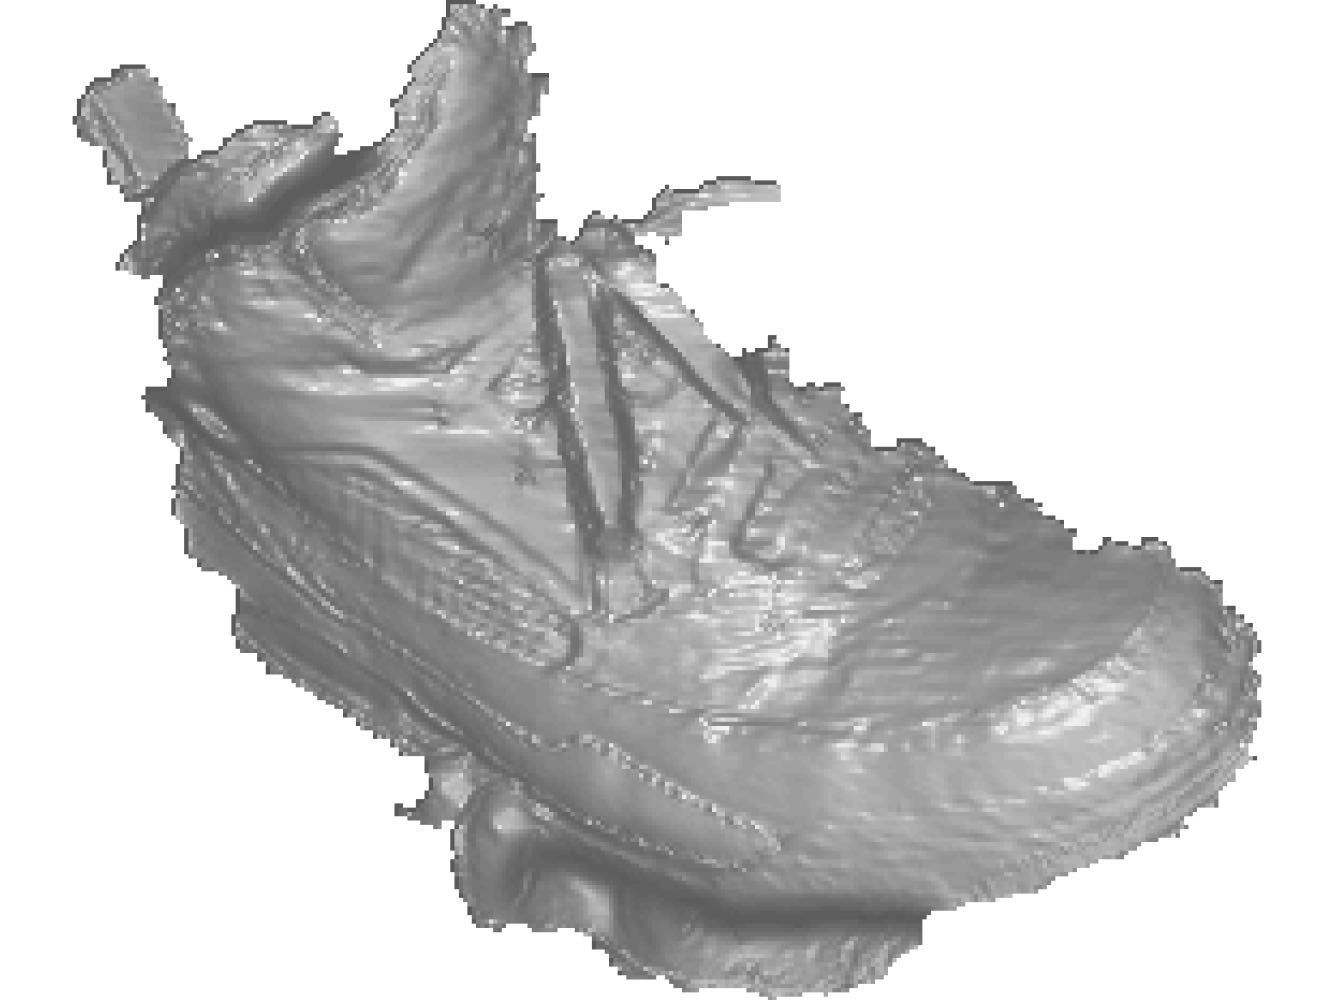
\includegraphics[height = 0.19\linewidth]{figures/methodology/ratio_shoe_shape.pdf} \\

   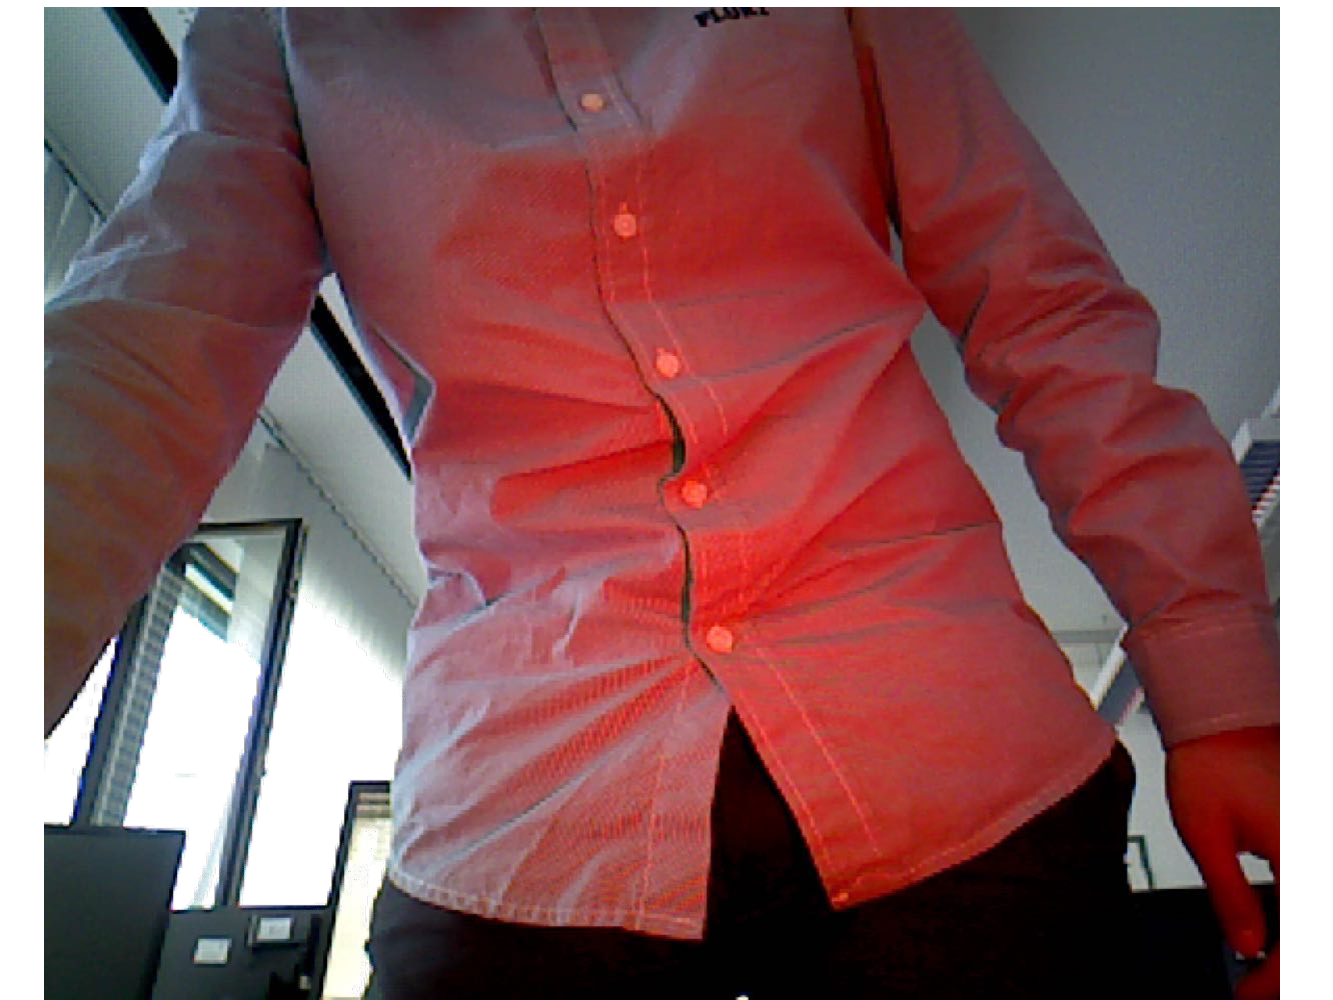
\includegraphics[height = 0.19\linewidth]{figures/methodology/ratio_shirt_rgb.pdf} 
   &
   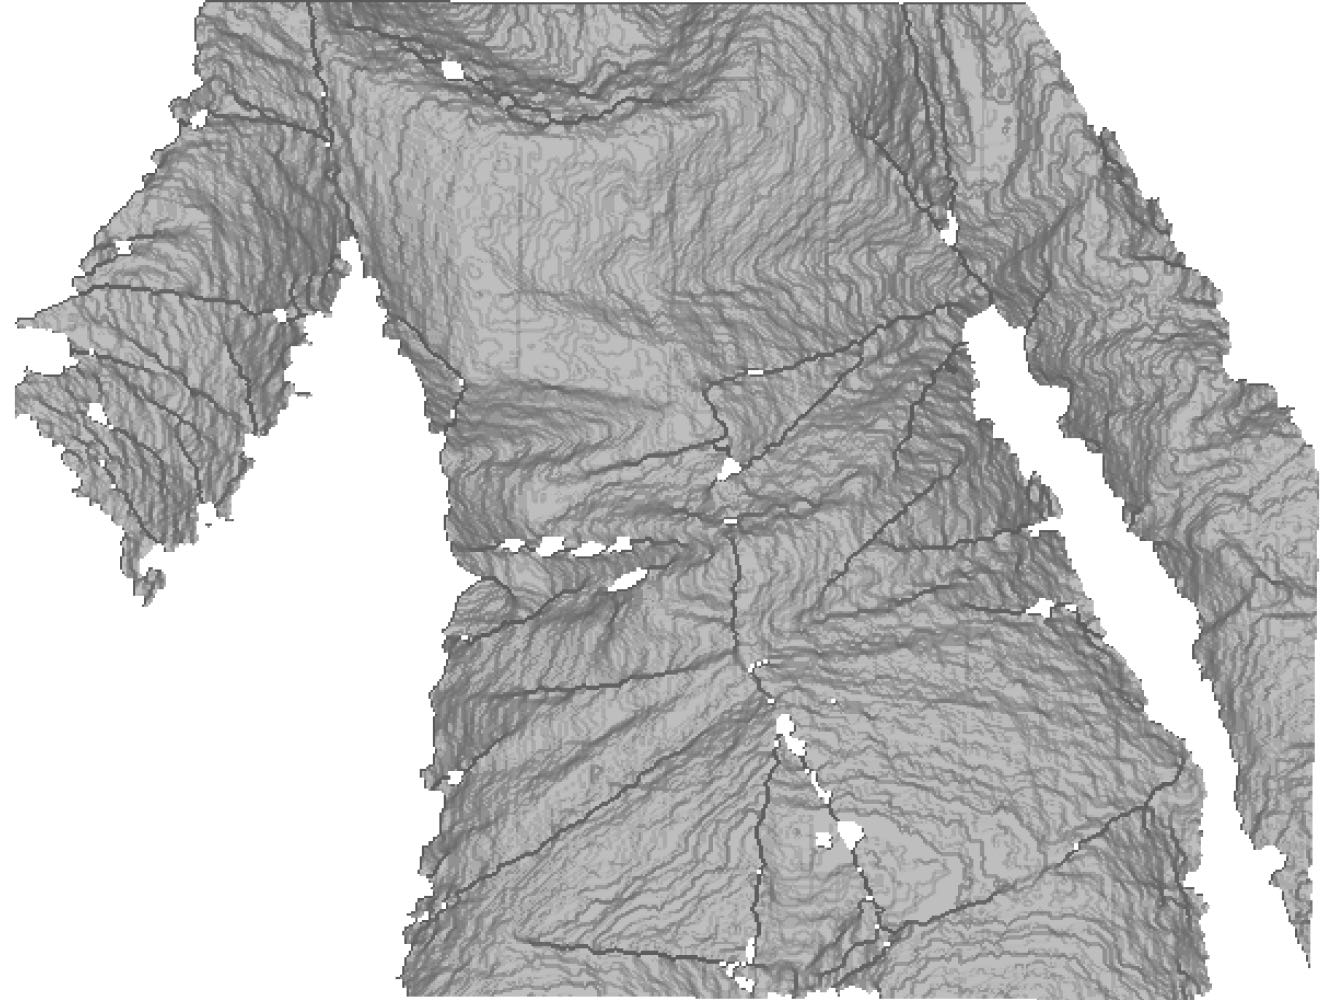
\includegraphics[height = 0.19\linewidth]{figures/methodology/ratio_shirt_shape_init.pdf} &
   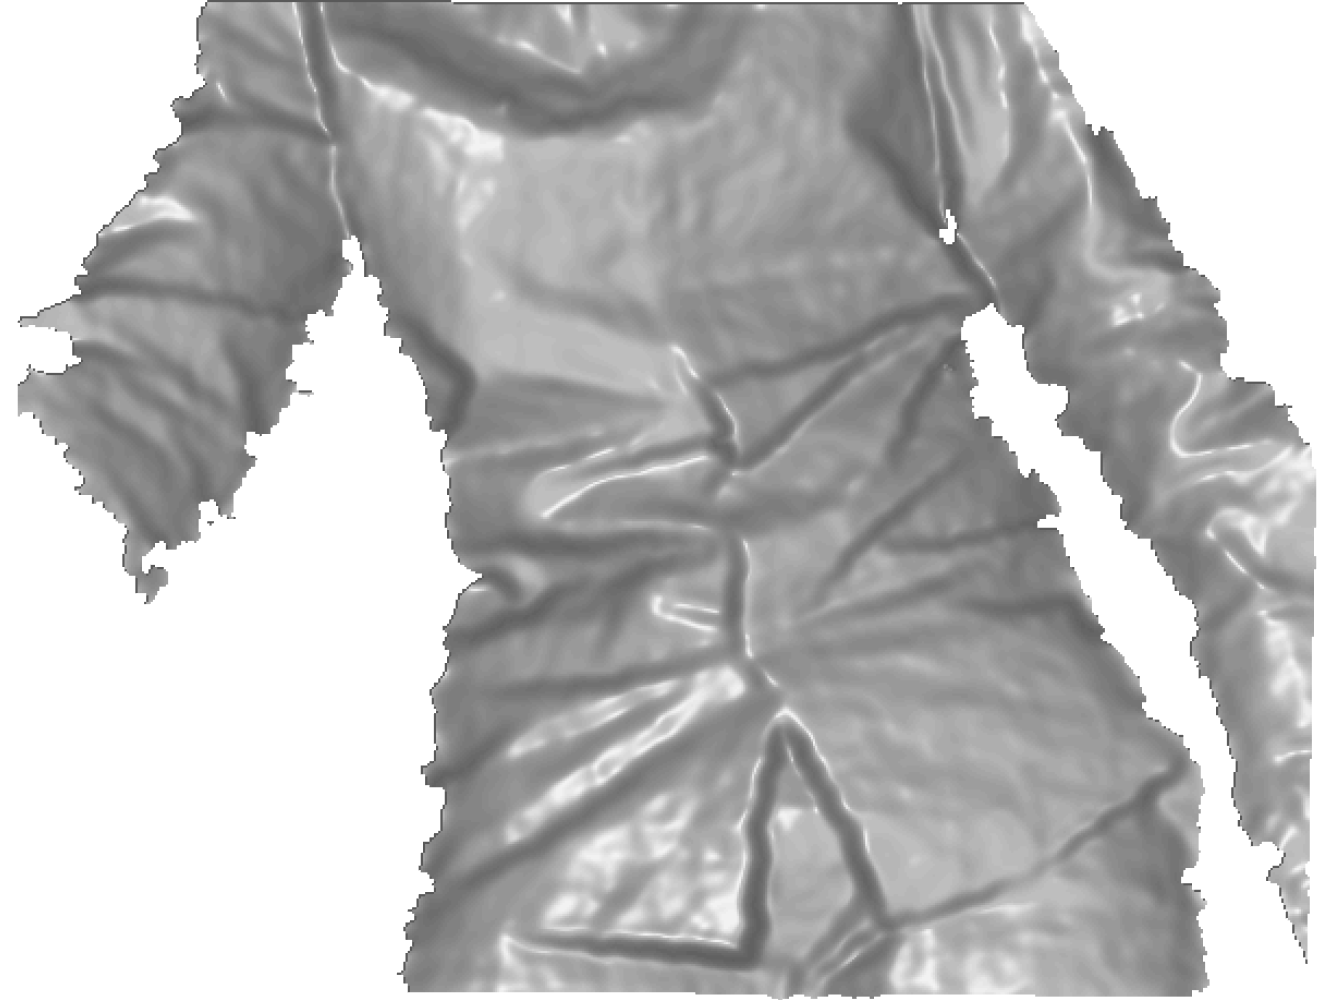
\includegraphics[height = 0.19\linewidth]{figures/methodology/ratio_shirt_shape_smooth.pdf} &
   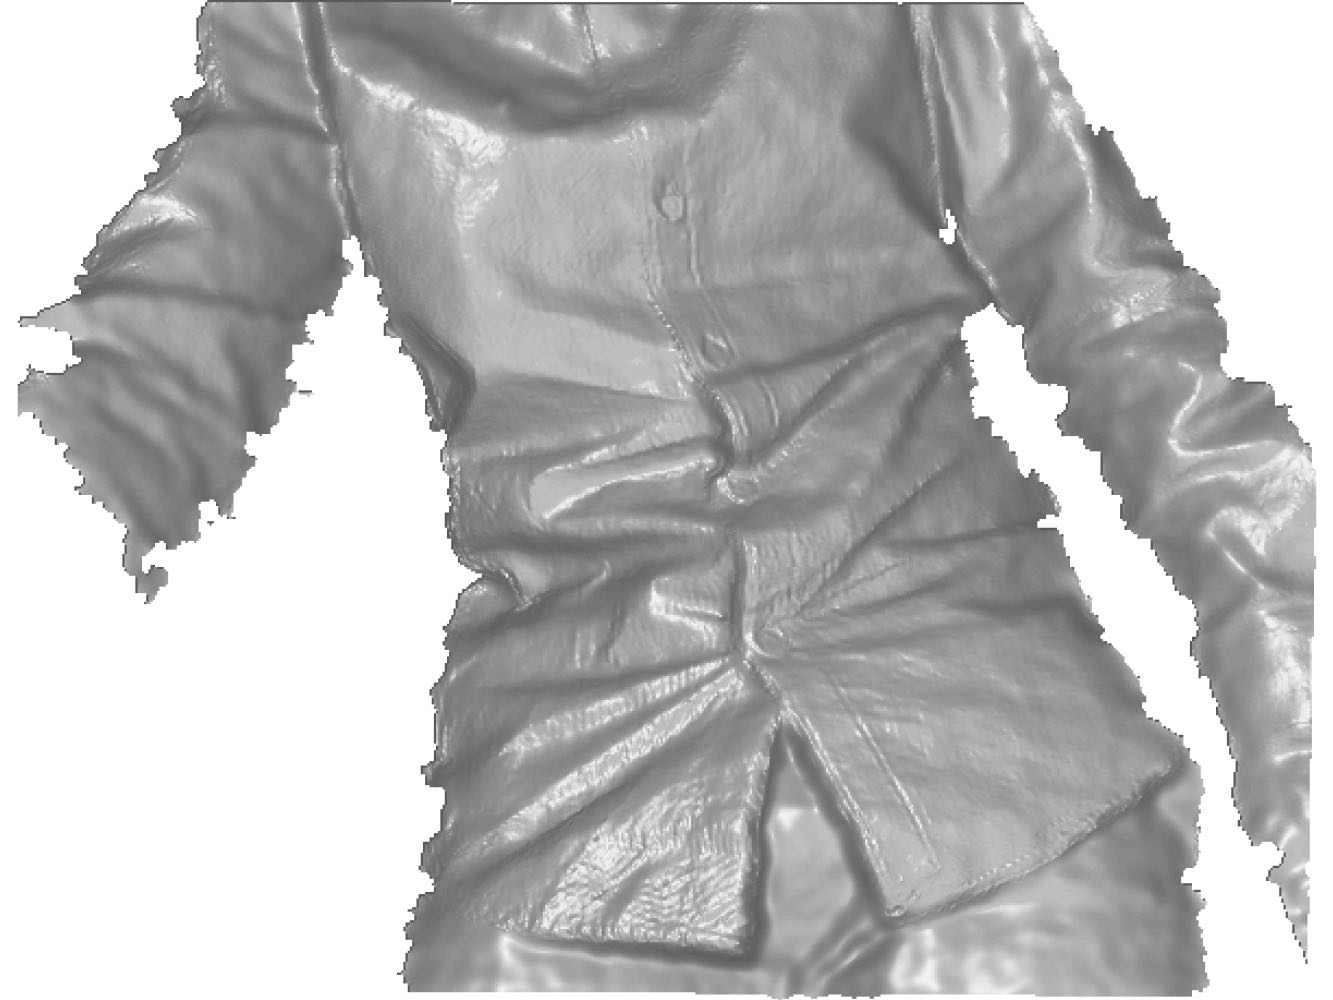
\includegraphics[height = 0.19\linewidth]{figures/methodology/ratio_shirt_shape.pdf} \\

   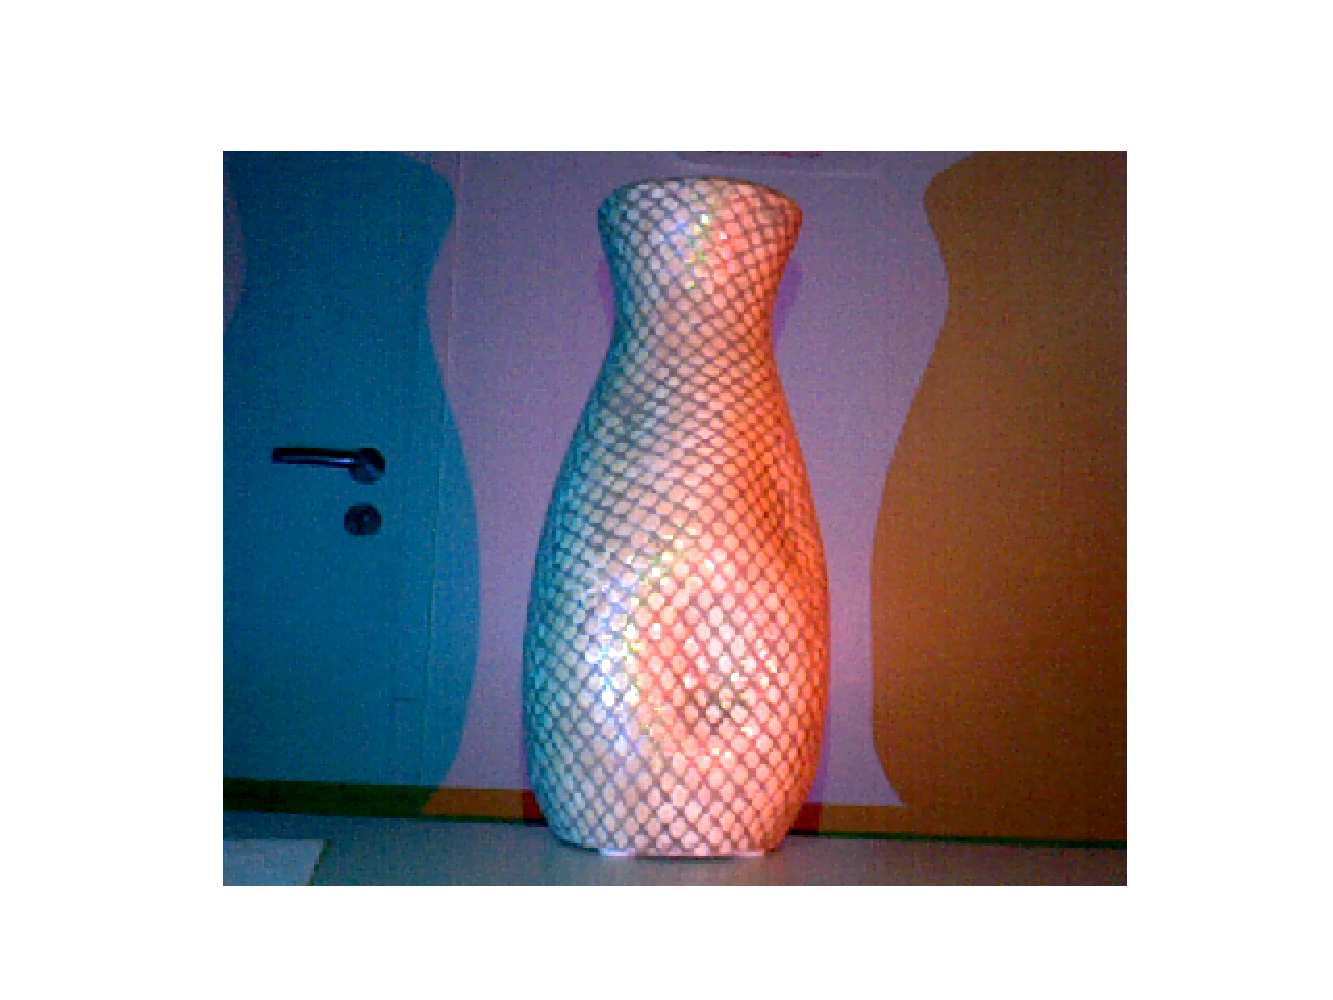
\includegraphics[height = 0.19\linewidth]{figures/methodology/ratio_vase_rgb.pdf}
   &
   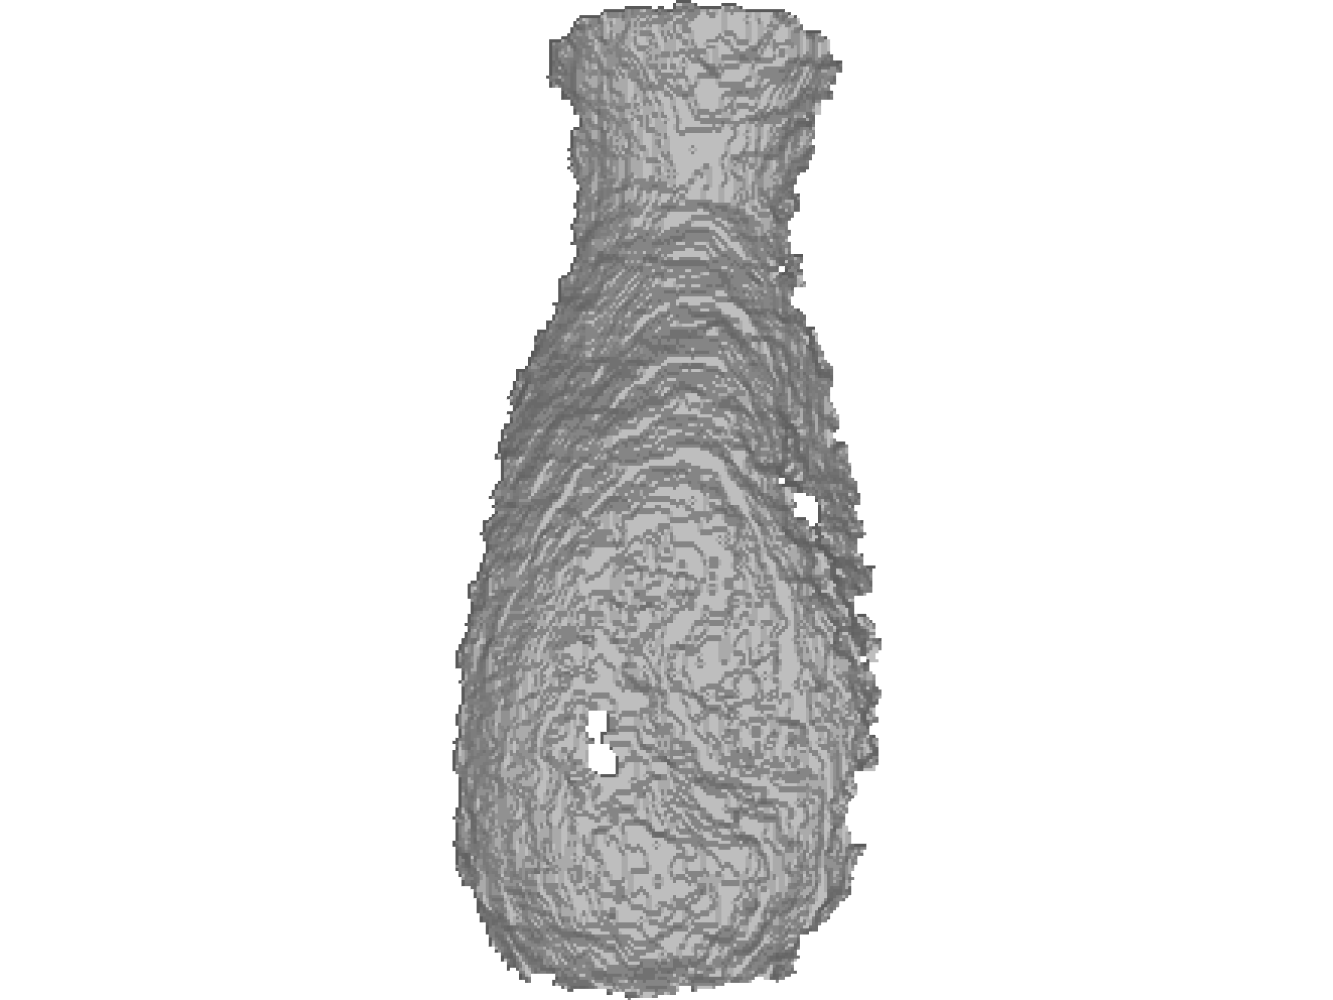
\includegraphics[height = 0.19\linewidth]{figures/methodology/ratio_vase_shape_init.pdf} &
   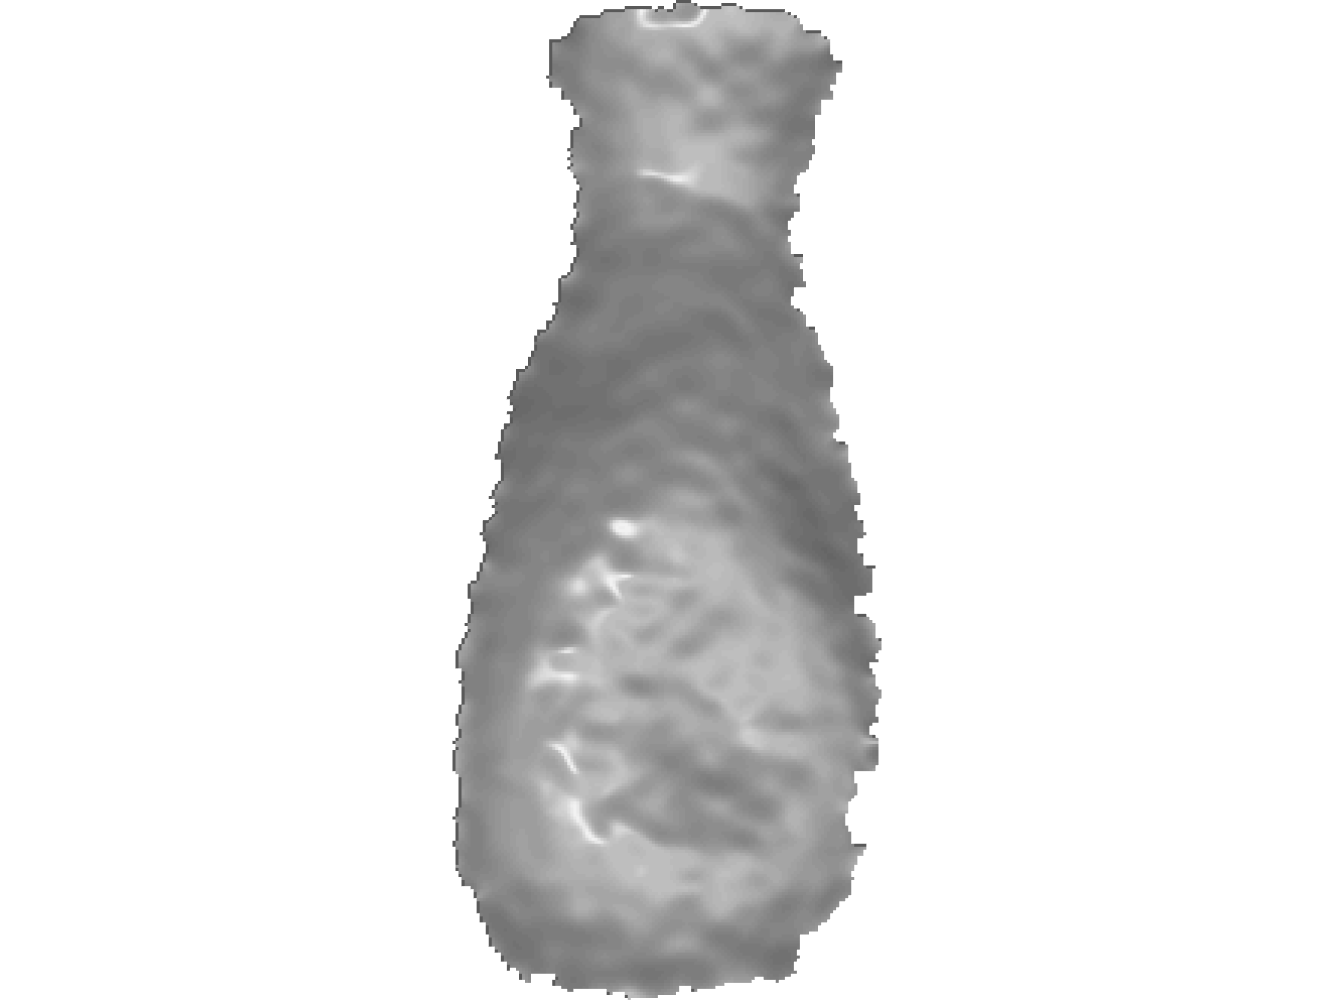
\includegraphics[height = 0.19\linewidth]{figures/methodology/ratio_vase_shape_smooth.pdf} &
   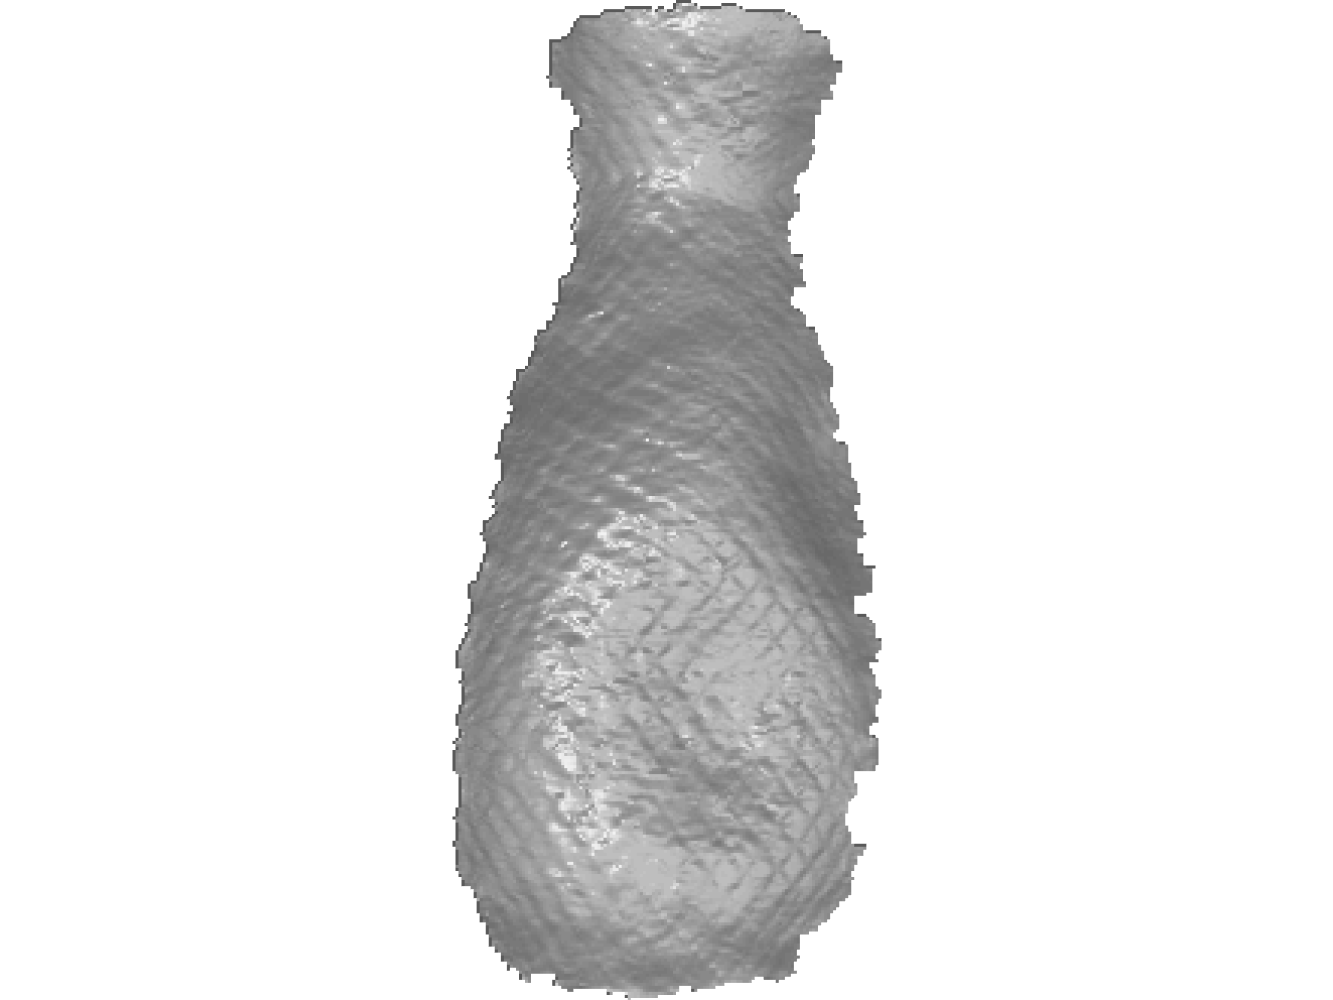
\includegraphics[height = 0.19\linewidth]{figures/methodology/ratio_vase_shape.pdf} \\      {RGB image} & {Input depth} & {After pre-processing} &{Refined depth}                 
 \end{tabular}}
\caption{Illustrations for the depth refinement of our proposed RGB ratio model. It should be mentioned that the middle row was under the natural scene illumination and our method still works well.}
\label{fig:ratio_illustration}
\end{figure}
%&&&&&&&&&&&&&&&&&&&&&&&&&



%----------------------------------------------
\subsection{Limitations}
%----------------------------------------------
Our method can estimate the albedo and the depth better than our RGBD-Fusion like method in some cases because the non-linearity optimization problem for the RGBD-Fusion like method has been solved.
Still, there exist some defects for our new RGB ratio model.
\begin{itemize}
\item Three LED lights have to be set up far away from each other.
	As already mentioned about Eq.~\ref{eq:ratio_albedo_prepare} , the albedo refinement may fail if the lights are too close and thus, we need to put 3 lights too near. 
	This can lead to some inconvenience, such as the requirement of enough space to put the system.
\item RGB three lights is likely to bring extra specularity.
	 If we want to refine the depth of an specular objects, the specular reflection will be from not only the natural scene illumination, but also RGB lights from 3 directions, which will make the refined results even worse.
	 
\item Auto white balance (AWB) has a big impact on the refined results.
	This is due to the fact that the success of our model highly relies on the difference among 3 channels in a color image.
	And AWB will mix up the information in 3 channels so it is very necessary to turn it off.
	This impedes the generalization of our model because AWB has been set as a default in many modern inexpensive cameras.
\end{itemize}


%%%%%%%%%%%%%%%%%%%%%%%%%%%%%%%%%%%%%%%%%%%%
\section{Proposed method II: Robust Multi-Light Model}

%----------------------------------------------
\subsection{Inspiration}
%----------------------------------------------
We can notice that the albedo estimation of both our RGBD-Like method and RGB ratio model is highly dependent on the regularization terms which emphasize the piece-wise smoothness.
This is a standard approach for almost all the state-of-the-art depth refinement method to estimate the albedo.
They work fine when the albedo itself is very simple with big patches of patterns and only several dominant colors.
However, there are more real-world objects containing complicated layout colors and patterns which all these methods with such a process of albedo estimation will fail.
Were the albedo estimation not working, the outcome of final depth refinement has no chance to be corrrect. 
What is more, The parameters for the regularization terms are often needed to be different for various object, so the parameters tuning for the regularization is tedious and time-consuming.

As a consequence, it is reasonable to propose a new method which is able to eliminate all the regularization terms and estimate complicated albedo.
The necessity of using regularizations for calculating albedo have been mentioned in section~\ref{sec:rgbd_albedo_estimation}, which in short is about avoiding the overfitting problem if only the shading term is applied.
Provided we have several color images for a still object with light coming from various directions, the shading term in Eq.~\ref{eq:rgbd_albedo_estimate} without the need of regularizations is sufficient for estimating the albedo.
{\color{blue} (not sure) Assuming the $n$ lights directions are estimated while the rough surface normal and $n$ color images are given, in this case, computing the albedo with a least square can resolve the overfitting problem.}

In order to simulate the scenario that a direct light comes from different directions, we simply sway a white LED light in different directions and take several images (even just the flash lamp on any phone is okay). An example of a vase from different lighting directions are shown in Fig.~\ref{fig:robust_setup}.

\begin{figure}[!htbp]
\centering
\subfigure{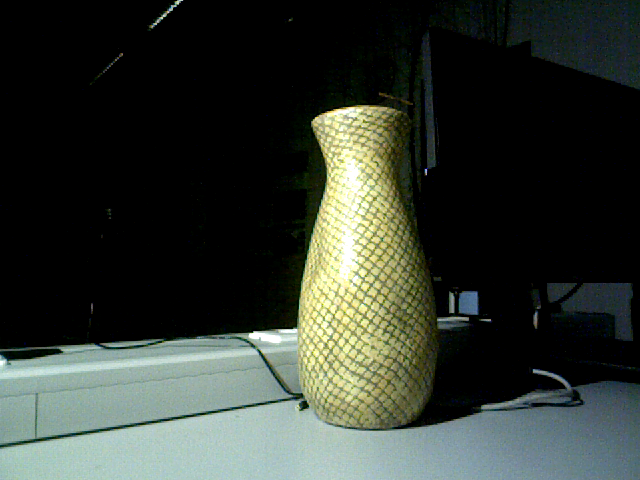
\includegraphics[width=0.23\linewidth]{figures/methodology/robust_setup1.png}}
\subfigure{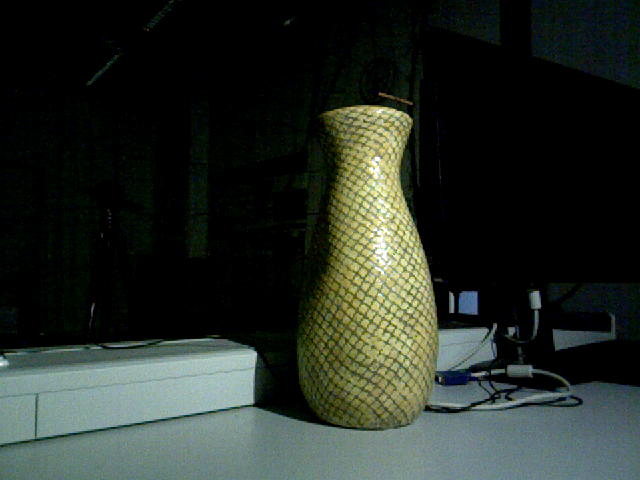
\includegraphics[width=0.23\linewidth]{figures/methodology/robust_setup2.png}}
\subfigure{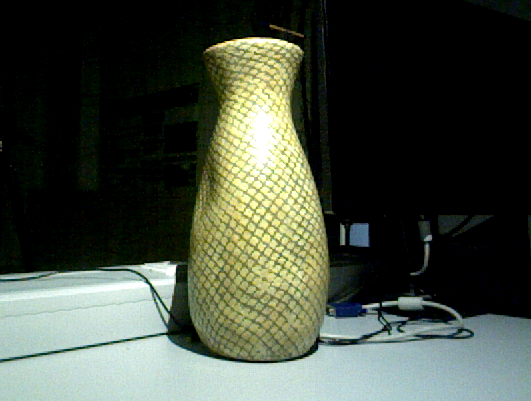
\includegraphics[width=0.23\linewidth]{figures/methodology/robust_setup3.png}}
\subfigure{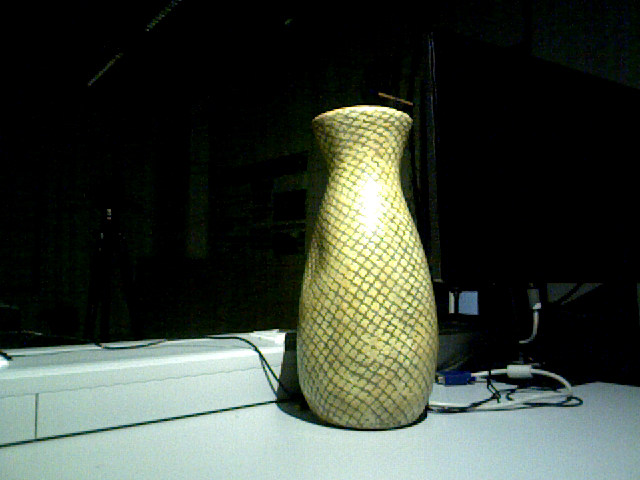
\includegraphics[width=0.23\linewidth]{figures/methodology/robust_setup4.png}}
\caption{Illustrations for the obtained color images of a vase from various light directions with a white LED light.}
\label{fig:robust_setup}
\end{figure}
 
{\color{red} put a real-world albedo estimate case that RGBD-fusion fails but our method works}


%----------------------------------------------
\subsection{Algorithm details}
%----------------------------------------------
Since we don't control with RGB LED lights anymore but one white light, the ratio model in Eq.~\ref{eq:ratio_rg_sh1} is not applicable anymore, so we need to use the standard 1st-order SH model described in Eq.~\ref{eq:rgbd_light_model} again to construct the input color images.

Again, the proposed algorithm consists of three parts: light estimation, albedo estimation and depth enhancement. 
We need to iteratively update the light directions, color albedo and the depth, but unlike the RGB ratio model method, we don't need to have an initial estimated light and albedo beforehand.
Instead, we can just assume the albedo to be 1 everywhere at the beginning and then start refining everything reiteratively in the loop, as shown in Alg.~\ref{alg:robust}.

First of all, the SFS model we use for the proposed method is still from Eq.~\ref{eq:rgbd_light_model}, so the corresponding SFS minimization problem now becomes:
%$$$$$$$$$$$$$$$$$
\begin{equation}
    \sum_{i} \sum_{c} \mathop{\sum \sum}_{(x,y) \in \mathcal{M}} |\rho_c(x,y) \mathbf{s}_{i,c}^\top\tilde{\mathbf{n}}(x,y) - I_{i,c}(x,y)|^2 
\end{equation}
%$$$$$$$$$$$$$$$$$
$c\in\{R,G,B\},\; i\in\{ 1, \cdots, n\}$, where $n$ stands for the total number of varying light directions.
A simplified version of the SFS energy is:
%$$$$$$$$$$$$$$$$$
\begin{equation}
    \sum_{i} \sum_{c} \lVert\rho_c \cdot \tilde{\mathbf{n}}\mathbf{s}_{i,c} -  I_{i,c} \rVert_2^2 
\end{equation}

Now the overall energy for our proposed robust multi-light method is characterized as:

%$$$$$$$$$$$$$$$$$
\begin{equation}\label{eq:robust_energy}
    E(\rho, z, \mathbf{s}) = \sum_{i} \sum_{c} \lVert \rho_c \cdot \tilde{\mathbf{n}}(z)\mathbf{s}_{i,c}  - I_{i,c}\rVert_2^2  + \lambda_{z}\lVert z - z_0 \rVert_2^2
\end{equation}
%$$$$$$$$$$$$$$$$$
As we can notice, the new overall energy is extremely simple with only one SFS term and one depth fidelity term, no any regularization terms for the albedo or depth estimation.
And we have found out that $\lambda_z = 0.01$ works really well for all cases, which means our system can be used by anybody easily without problems.

\textbf{Light estimation}
In each iteration, we first freeze the albedo and the surface normal and then refine the SH parameters for all input images from the overall energy in Eq.~\ref{eq:robust_energy}.
%%$$$$$$$$$$$$$$$$$
%\begin{equation}\label{eq:robust_light_estimate}
%    \min_{\mathbb{S}_c} \; \sum_{c} \lVert \mathbb{I}_c - \rho_c \mathbb{S}_{c}\tilde{\mathbf{n}}\rVert_2^2
%\end{equation}
%$$$$$$$$$$$$$$$$$
To estimate the light with the simple least squares, we need to reshape the SFS term to a linear problem with the SH light as the argument. 

First of all, to further simplify the energy, we define $\mathbb{I}_c$ and $\mathbf{S}_c$ as:
%$$$$$$$$$$$$$$$$$
\begin{equation}\label{eq:robust_energy_prepare}
\mathbb{I}_c = \begin{pmatrix} I_{1,c} \\ \vdots \\ I_{n,c} \end{pmatrix}  \; \; \mathbf{S}_c = \begin{pmatrix} \mathbf{s}_{1,c} \\ \vdots \\ \mathbf{s}_{n,c} \end{pmatrix}
\end{equation}
%$$$$$$$$$$$$$$$$$
$\mathbb{I}_c \in \mathbb{R}^{mn}, \mathbf{S}_c \in \mathbb{R}^{4n}$.
And then we define a multiplication operator $\odot$ between any matrix $\mathbf{A}$ and vector $\mathbf{b}$ with the same number of rows, $\mathbf{C = A \odot b}$.
$\mathbf{C}$ is the result of the element-wise multiplication between each column of $\mathbf{A}$ and $\mathbf{b}$.
Now we have a vector $\rho_c\in \mathbb{R}^m$ and a matrix $\tilde{\mathbf{n}} \in \mathbb{R}^{m \times 4}$, where $m$ represents the number of pixel inside the mask $\mathcal{M}$.
So we repeat the resulted matrix $\tilde{\mathbf{n}} \odot \rho_c$ on the diagonal of a big sparse matrix $\mathbf{A}_{\mathbb{S}_c} \in \mathbb{R}^{mn \times 4n}$, whose structure is illustrated in Fig.~\ref{fig:robust_matrix1}.
The Eq.~\ref{eq:robust_energy} now is reformulated as:
%$$$$$$$$$$$$$$$$$
\begin{equation}\label{eq:robust_light_estimate2}
    \min_{\mathbf{S}_c} \; \sum_{c} \lVert \mathbf{A}_{\mathbf{s}_c}\mathbf{S}_c  - \mathbb{I}_c \rVert_2^2
\end{equation}
%$$$$$$$$$$$$$$$$$

\textbf{Albedo estimation}
Similar to the light estimation, we need to reshape the SFS term in the overall energy in order to solve with least squares.
The energy for the albedo estimation from the overall energy looks like this:
%$$$$$$$$$$$$$$$$$
\begin{equation}\label{eq:robust_albedo_estimate}
	\min_{\rho_c} \; \sum_{c}\lVert \mathbf{A}_{\rho_c}\rho_c - \mathbb{I}_c \rVert^2_2 
\end{equation}
%$$$$$$$$$$$$$$$$$
$ \mathbf{A}_{\rho_c} \in \mathbb{R}^{mn \times m}$ is the stack of $n$ diagonal matrices $\text{diag}(\tilde{\mathbf{n}} \cdot \mathbf{s}_{i,c})$, where $\text{diag} : \mathbb{R}^m \rightarrow \mathbb{R}^{m\times m}, i \in \{1, \cdots, n\}$.
A toy example of $\mathbf{A}_{\rho_c}$ with $n=6$ is illustrated in Fig.~\ref{fig:robust_matrix2}.

\begin{figure}[!ht]
\centering
\subfigure[An example of $\mathbb{A}_{\mathbb{S}_c}$ with $n = 6$. The yellow part represents the repetition of matrix $\tilde{\mathbf{n}} \odot \rho_c$]{\label{fig:robust_matrix1}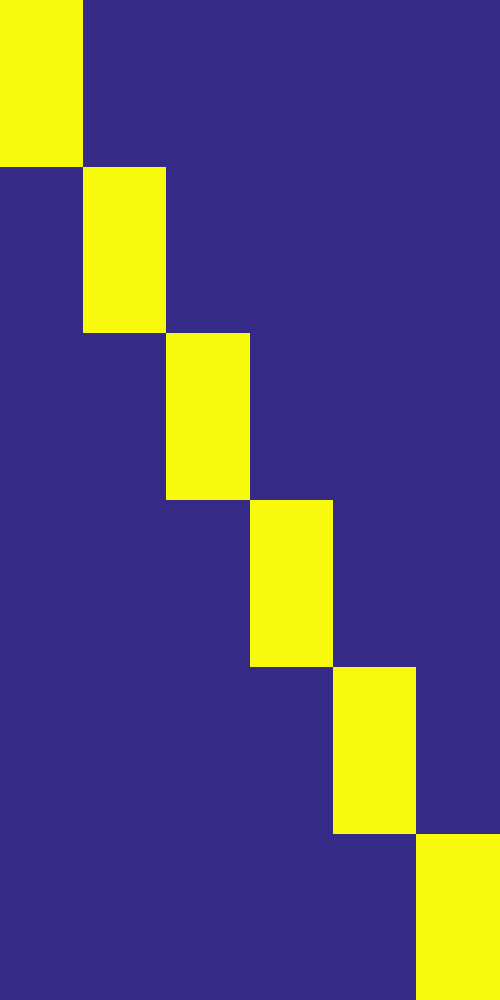
\includegraphics[width=0.3\linewidth]{figures/methodology/As_matrix.pdf}}
\quad
\subfigure[An example of $\mathbb{A}_{\rho_c}$ with $n = 6$. Every yellow line represents $\text{diag}(\tilde{\mathbf{n}} \cdot \mathbf{s}_{i,c})$]{\label{fig:robust_matrix2}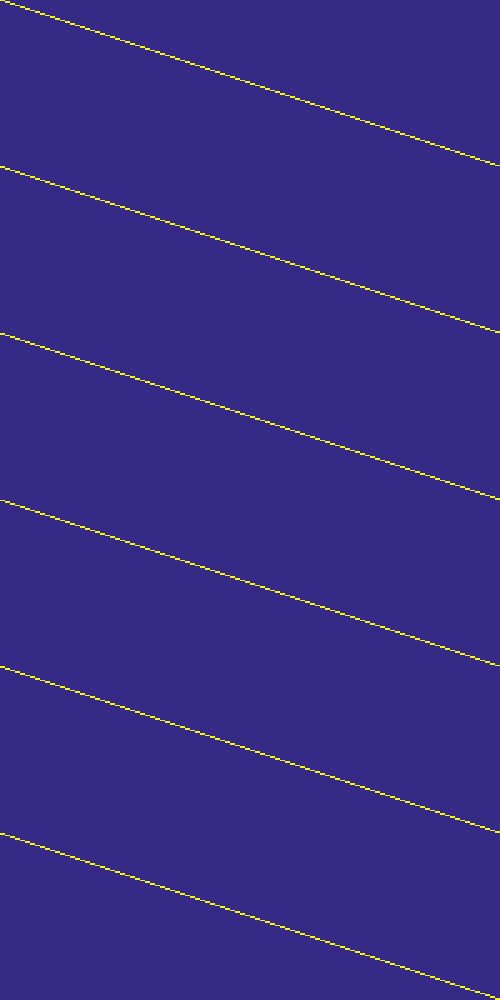
\includegraphics[width=0.3\linewidth]{figures/methodology/Ap_matrix.pdf}}

\caption{Illustrations for the structures of the matrices $\mathbb{A}_{\mathbb{S}_c}$ and $\mathbb{A}_{\rho_c}$. The number of different light conditions is $n = 6$.}
\label{fig:robust_matrix}
\end{figure}

\textbf{Depth enhancement}
After having the estimated light and the color albedo, we can continue refining the depth.
Again, we need to rearrange the energy function with the depth $z$ as the argument.
First, let us start from the simplest case and consider one pixel in one of the input images.
If we expand Eq.~\ref{eq:rgbd_light_model} with the the perspective projection normal in Eq.~\ref{eq:ratio_normal}, we have:
%$$$$$$$$$$$$$$$$$
\begin{equation}
    I(x,y) = \rho(x,y) \cdot \; 
    \begin{pmatrix}
        l^1 & l^2 & l^3 
    \end{pmatrix}
     \begin{pmatrix}
         fz_x(x,y)\\
         fz_y(x,y)\\
         -1 - (x - x_0)z_x(x,y) - (y - y_0)z_y(x,y)
     \end{pmatrix}/ d(x,y)
     + \rho(x,y) \cdot \varphi   
\end{equation}
%$$$$$$$$$$$$$$$$$
where $d = \sqrt{(fz_x(x,y))^2 + (fz_y(x,y))^2 + (-1 - (x - x_0)z_x(x,y) - (y - y_0)z_y(x,y))^2}$ is a normalizer.
After rearranging, we have:
 %$$$$$$$$$$$$$$$$$
\begin{equation}
    \frac{l^1f - l^3(x-x_0)}{d(x,y)}z_x(x,y) + \frac{l^2f - l^3(y-y_0)}{d(x,y)}z_y(x,y) = I(x,y) + \frac{l^3}{d(x,y)} - \rho(x,y)\varphi
\end{equation}
 %$$$$$$$$$$$$$$$$$
If we extend this to the whole pixel in the mask $\mathcal{M}$, the equation becomes:
 %$$$$$$$$$$$$$$$$$
\begin{equation}\label{eq:robust_depth1}
    \frac{l^1f - l^3\tilde{x}}{d} \cdot z_x + \frac{l^2f - l^3\tilde{y}}{d} \cdot z_y = I + \frac{l^3}{d} - \varphi \cdot \rho
\end{equation}
Provided we have the gradient matrices in $x$ and $y$ directions denoted roughly as:
 %$$$$$$$$$$$$$$$$$
\begin{equation}
D_x = \begin{pmatrix}
-1 & 1 & 0 &\cdots & 0 & 0 \\
0 & -1 & 1 &\cdots &  0 & 0 \\
\vdots & \vdots & \ddots & \ddots & \vdots & \vdots \\
0 & 0 & 0 & \cdots & -1 & 1
\end{pmatrix}_{m\times m}
\quad
D_y = \begin{pmatrix}
-1 & 0 & \cdots & 0 \\
1 & -1 & \cdots & 0 \\
0 & 1 & \ddots & 0 \\
\vdots & \vdots & \ddots & \vdots\\
0 & 0 & \cdots & -1\\
0 & 0 & \cdots & 1
\end{pmatrix}_{m\times m}
\end{equation}
 %$$$$$$$$$$$$$$$$$
Then Eq.~\ref{eq:robust_depth1} becomes:
 %$$$$$$$$$$$$$$$$$
\begin{equation}\label{eq:robust_depth2}
        [\text{diag}(\frac{l^1f - l^3\tilde{x}}{d}) D_x + \text{diag}(\frac{l^2f - l^3\tilde{y}}{d}) D_y] z = I + \frac{l^3}{d} - \varphi \cdot \rho
\end{equation}
 %$$$$$$$$$$$$$$$$$
This is the linear equation for one image. 
Now we define our $\mathbf{A}_z$ and $\mathbf{b}_z$ for our system:
 %$$$$$$$$$$$$$$$$$
\begin{equation}\label{eq:robust_depth3}
\begin{split}
    \mathbf{A}_{z_c} &= 
        \begin{pmatrix}    
            \text{diag}(\frac{l^1_{1,c}f - l^3_{1,c}\tilde{x}}{d_1}) D_x + \text{diag}(\frac{l^2_{1,c}f - l^3_{1,c}\tilde{y}}{d_1}) D_y \\
            \vdots \\
            \text{diag}(\frac{l^1_{n,c}f - l^3_{n,c}\tilde{x}}{d_n}) D_x + \text{diag}(\frac{l^2_{n,c}f - l^3_{n,c}\tilde{y}}{d_n}) D_y \\
        \end{pmatrix}_{mn \times m}
\\
    \mathbf{b}_{z_c} &=     
        \begin{pmatrix}    
            I_{1,c} + \frac{l^3_{1,c}}{d_{1}} - \varphi_{1,c} \cdot \rho_{c} \\
            \vdots\\
            I_{n,c} + \frac{l^3_{n,c}}{d_{n}} - \varphi_{n,c} \cdot \rho_{c} \\
        \end{pmatrix}_{mn \times 1}    
\end{split}
\end{equation}
 %$$$$$$$$$$$$$$$$$
 It worths mentioning that in each iteration, we freeze $d$ with $z$ from last iteration, so the non-linearity is solved.
 Finally, we have stack $\mathbf{A}_{z_c}$ and $\mathbf{b}_{z_c}$ for each channel $c\in\{R,G,B\}$:
 %$$$$$$$$$$$$$$$$$
 \begin{equation}
     \mathbf{A}_z = 
         \begin{pmatrix}
             \mathbf{A}_{z_R}\\
             \mathbf{A}_{z_G}\\
             \mathbf{A}_{z_B}
         \end{pmatrix},\quad
     \mathbf{b}_z = 
         \begin{pmatrix}
             \mathbf{b}_{z_R}\\
             \mathbf{b}_{z_G}\\
             \mathbf{b}_{z_B}
         \end{pmatrix}         
 \end{equation}
 %$$$$$$$$$$$$$$$$$
After all the derivations, we finally model our energy for the depth enhancement as:
 %$$$$$$$$$$$$$$$$$
 \begin{equation}\label{eq:robust_depth_estimate}
	\min_{z} \; \lVert  \mathbf{A}_{z}z - \mathbf{b}_z\rVert^2_2 + \lambda_{z}\lVert z - z_0 \rVert_2^2
\end{equation}
The conjugate gradient (CG) method has been applied to optimize all three sub energy.
And the structure of the proposed algorithm is described in Alg.~\ref{alg:robust} and one refined depth result is shown in Fig.~\ref{fig:robust_illustration}.
More examples can be found in chapter~\ref{chap:result}.
 %$$$$$$$$$$$$$$$$$

\begin{algorithm}[!htbp]
	\begin{algorithmic}[1] 
  		\caption{\textbf{Robust Multi-Light Model Method}}
		\label{alg:robust}
		 \renewcommand{\algorithmicrequire}{\textbf{Input:}}
		 \renewcommand{\algorithmicensure}{\textbf{Output:}}
		 \REQUIRE Initial depth image $z_0$, RGB image $I$, mask, focal length, principle point
		 \vspace{1.8mm}
		 \STATE t = 1, $z^{(t-1)} = z_0$, $\rho^{(0)}_R, \rho^{(0)}_G, \rho^{(0)}_B = 1$
		 \vspace{1.8mm}
		  \WHILE {$ \frac{\Vert E(\rho^{(t)}, z^{(t)}, \mathbf{s}^{(t)}) - E(\rho^{(t-1)}, z^{(t-1)}, \mathbf{s}^{(t)})\Vert}{E(\rho^{(t-1)}, z^{(t-1)}), \mathbf{s}^{(t-1)}} > \epsilon$}
		       \vspace{1.8mm}
		        \STATE $\mathbf{s}^{(t)} = \argmin \limits_{\rho} E(\rho^{(t-1)}, z^{(t-1)})$ \COMMENT{Eq.~\ref{eq:robust_light_estimate2}}
			\STATE $\rho^{(t)} = \argmin \limits_{\rho} E(z^{(t-1)}, \mathbf{s}^{(t)})$ \COMMENT{Eq.~\ref{eq:robust_albedo_estimate}}
			  \STATE $z^{(t)} = \argmin \limits_{z} E(\rho^{(t)}, z^{(t-1)}, \mathbf{s}^{(t)})$ \COMMENT{Eq.~\ref{eq:robust_depth_estimate}}
			  \vspace{1.8mm}
		          \STATE $t := t + 1$
		 \vspace{1.8mm}
		  \ENDWHILE
		  \ENSURE  Refined depth image $z^{(t)}$ and albedo $\rho^{(t)}$
	\end{algorithmic}
\end{algorithm}




\begin{figure}[!ht]
\centering
\setlength{\tabcolsep}{0.2em} % column spacing
 {\renewcommand{\arraystretch}{0.9}% row spacing
\begin{tabular}{c| c c}
   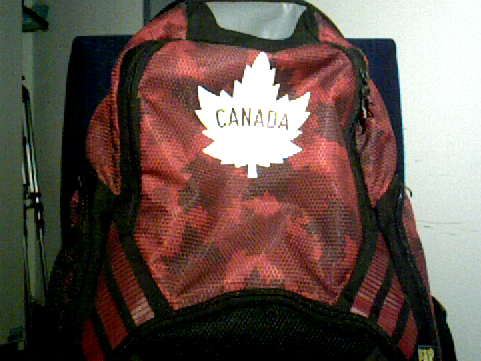
\includegraphics[height = 0.25\linewidth]{figures/methodology/robust_backpack_rgb.png}&
   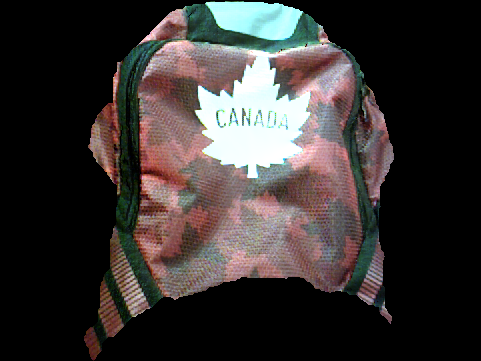
\includegraphics[height = 0.25\linewidth]{figures/methodology/robust_backpack_rho.png} &
   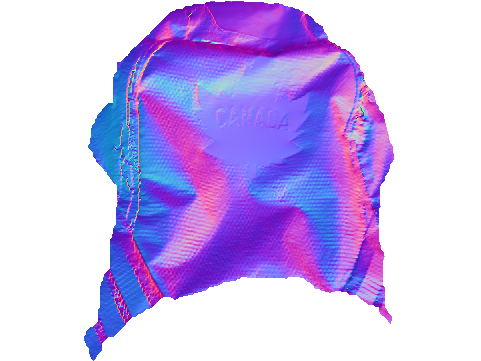
\includegraphics[height = 0.25\linewidth]{figures/methodology/robust_backpack_normal.png} \\
   {Backpack} & {Estimated albedo} & {Refined normal}\\
   \includegraphics[height = 0.25\linewidth]{figures/methodology/robust_backpack_shape_init.pdf}&
   \includegraphics[height = 0.25\linewidth]{figures/methodology/robust_backpack_shape_smooth.pdf}&
   \includegraphics[height = 0.25\linewidth]{figures/methodology/robust_backpack_shape.pdf}\\
{Input depth} & {After pre-processing} & {Refined depth}
 \end{tabular}}
\caption{Illustrations for our proposed robust multi-light method. Here $n = 10$ images with various lighting conditions have been used, one of which is the top left RGB image. }
\label{fig:robust_illustration}
\end{figure}
%&&&&&&&&&&&&&&&&&&&&&&&&&




%----------------------------------------------
\subsection{When super-resolution meets depth refinement}
%----------------------------------------------
We can notice that there exist over-smoothed problem in many 3D scanning applications, which is due to the fact that the depth map given by the consumer RGBD-camera usually has a really low resolution.
The scanning or reconstruction results will be then improved if the depth resolution is increased.
And as we know, for most of the well-known comsumer RGB-D cameras the depth resolution is far smaller than the RGB resolution.
For instance, ASUS Xtion Pro Live can acquire $1280\times 1024$ RGB images and $640\times 480$ depth images. Microsoft Kinect 2.0 owns $1920\times1080$ RGB resolution but only $512\times424$ depth one, and Intel RealSense R200 has a $1920\times1080$ RGB camera while the depth reoslution is $640\times 480$.
It would be very useful if we can not only refine the depth map in its original scale, but close to the RGB resolution.  

In this section, we will present our approach of the combination of the photometric stereo and super-resolution, with the help of which we will provide satisfying high-quality and high-resolution depth maps. 

The scale factor between the RGB and depth image is around $2$ for ASUS XtionPro Live, so we can at least enlarge our map two times larger than the original size, which means the refined depth resolution will be $1280\times960$.
 And we assume that the input depth image has been registered well (done easily with OpenNI) such that the upsampled depth $Z$ is aligned with the large RGB image after simple interpolation.

Assuming the acquired small depth and the super-resolution depth are denoted as $z$ and $Z$ respectively.
A standard single depth image super-resolution problem can be represented like in~\cite{yang2010image}:
\begin{equation}\label{eq:sr_equation}
z = KFZ
\end{equation}
where $K$ represents a downsampling operator and $F$ a blurring filter.
For the sake of simplicity we don't consider the filter $F$ but only a simple downsampling operator.
If we the $z$ and $Z$ are vectorized, the $K$ turns to a matrix, which we choose a native 4-connected isotropic downsampling matrix.

In the light, albedo estimation part, the energy in Eq.~\ref{eq:robust_light_estimate2} and Eq.~\ref{eq:robust_albedo_estimate} are directly used. When we build $\mathbf{A}_{\mathbf{s}_c}$ and $\mathbf{A}_{\rho_c}$, the surface normal $\mathbf{n}(z)$ is replaced with $\mathbf{N}(Z)$ which is the normal of the large depth. 
However, the depth enhancement part with Eq.~\ref{eq:robust_depth_estimate} should be adapted to the super-resolution framework. 
As we know, the super-resolution equation in Eq.~\ref{eq:sr_equation} is ill-posed so our SFS term can be treated as the regularization term.
Now, $Z$ is again used to replace $z$ during the construction of $\mathbf{A}_z$ and $\mathbf{b}_z$, which are now denoted by $\mathbf{A}_Z$ and $\mathbf{b}_Z$.
 
With the input small depth $z_0\in\mathcal{R}^m$ and a downsampling kernal $K \in \mathbb{R}^{m\times M}$ where $M$ and $m$ represent the number of pixel within the big mask and the small mask respectively, The super-resolution depth refinement energy now is changed to:
 %$$$$$$$$$$$$$$$$$
 \begin{equation}\label{eq:robust_depth_estimate}
	\min_{Z} \; \lVert  \mathbf{A}_{Z}Z - \mathbf{b}_Z\rVert^2_2 + \lambda_{z}\lVert K\cdot Z - z_0 \rVert_2^2
\end{equation}
 %$$$$$$$$$$$$$$$$$
 After optimizing this energy, we will acquired super-resolution version refined depth, as illustrated in Fig.~\ref{fig:robust_sr}.
  \begin{figure}[!htbp]
\centering
\subfigure[One input image $(960\times1280)$]{\includegraphics[width=0.32\linewidth]{figures/methodology/sr_rgb_big.pdf}}
\subfigure[Estimated albedo $(960\times1280)$]{\includegraphics[width=0.32\linewidth]{figures/methodology/sr_albedo.pdf}}
\subfigure[Estimated normal$(960\times1280)$]{\includegraphics[width=0.32\linewidth]{figures/methodology/sr_normal.pdf}}
\subfigure[Input depth image $(480\times640)$]{\includegraphics[width=0.23\linewidth]{figures/methodology/sr_shape_before.pdf}}
\quad
\subfigure[Smoothed depth image $(480\times640)$]{\includegraphics[width=0.23\linewidth]{figures/methodology/sr_shape_smooth.pdf}}
\subfigure[Refined super-resolution depth $(960\times1280)$]{\includegraphics[width=0.46\linewidth]{figures/methodology/sr_shape_after.pdf}}
\caption{Results of the super-resolution depth of a paper bag. Input depth size is $480\times 640$, and the refined depth's is $960 \times 1280$.}
\label{fig:robust_sr}
\end{figure}


 
%%%%%%%%%%%%%%%%%%%%%%%%%%%%%%%%%%%%%%%%%%%%